\part{Appendices}

\chapter{Appendices for Chapter \ref{chap:comp}}
\label{app:comp}

\section{Selected hyperparameters for the classifiers and the baseline}
\label{app:comp:sec:selectedhyperparameters}

When we train a classifier on extracted features, we tune its hyperparameters by cross-validation. For SVM, we tune the penalty parameter $C$ with values taken in 
$\left\{10^{-10}, 10^{-9},...,10\right\}$. For extremely randomized trees, we grow fully expanded trees and tune the number of features evaluated at each split $k$ among $\left\{1, \sqrt{n_f}, \frac{n_f}{2}, n_f\right\}$ where 
$n_f$ is the total number of features. For the single layer perceptron, we tune the number of iterations among $\left\{1000, 2500, 5000, 10000\right\}$ and the learning rate among $\left\{10^{-4}, 10^{-3}, 10^{-2}, 10^{-1}\right\}$. All the other parameters values are the ones provided by default by the scikit-learn package \parencite{scikit-learn}. More precisely, we use: the Adam \parencite{kingma2014adam} optimizer with default parameters, an L2 penalty on the weights with $\alpha$ set to $10^{-4}$ and a batch size of 200 samples.

For the baseline ET-FL, we tune the size of the windows $\left(w_{min}, w_{max}\right)$ among all valid size ranges with \texttt{min\_size} in $\left\{0.0, 0.25, 0.5, 0.75\right\}$ and \texttt{max\_size} in $\left\{0.25, 0.5, 0.75, 1.0\right\}$ and the colorspace $L$ among $\left\{\texttt{TRGB}, \texttt{HSV}\right\}$ where \texttt{TRGB} and \texttt{HSV} are respectively the normalized RGB and hue-saturation-value colorspaces. The number of extracted subwindow per image $w$ is taken such that the total number of subwindows for the dataset $w_t$ is approximately 1 million. The other fixed parameters are $T$, the number of trees, $l_{min}$, the minimum number of samples in a leave of a tree. The value for those parameters as well as the selected values for tuned parameters are given in Table \ref{app:comp:tab:hyper_etfl}. 

\begin{table}
	\centering
	\begin{tabular}{|c|c|c|c|c|c|c|c|c|c|}
    	\hline
        \multirow{2}{*}{\textbf{Datasets}} & \multicolumn{6}{c|}{Fixed} & \multicolumn{3}{c|}{Tuned (best)} \\ 
     	\cline{2-10}
		 & $T$ & $w$ & $w_t$ & $l_{min}$ & $k$ & $C$ & $w_{min}$ & $w_{max}$ & $L$ \\ 
     	\hline
        C & 20 &  551 & 1000616 & 1000 & 384 & 0.01 & 0.25 & 0.50 & TRGB \\
        G & 20 &   69 & 1007745 & 1000 & 384 & 0.01 & 0.00 & 0.75 &  HSV \\
        P & 20 &  743 & 1000078 & 1000 & 384 & 0.01 & 0.25 & 0.50 &  HSV \\
        N & 20 & 1265 & 1000615 & 1000 & 384 & 0.01 & 0.00 & 0.25 &  HSV \\
        B & 20 &   55 & 1004355 & 1000 & 384 & 0.01 & 0.00 & 0.75 &  HSV \\
        M & 20 &  261 & 1001457 & 1000 & 384 & 0.01 & 0.25 & 0.75 & TRGB \\
        L & 20 &  184 & 1001512 & 1000 & 384 & 0.01 & 0.25 & 0.50 &  HSV \\
        H & 20 &  228 & 1002516 & 1000 & 384 & 0.01 & 0.25 & 0.50 & TRGB \\
     	\hline
	\end{tabular}
    \caption{Hyperparameters for ET-FL.}
    \label{app:comp:tab:hyper_etfl}
\end{table}

\section{Best features}
\label{app:comp:sec:bestfeatures}

In order to investigate the best features (according to feature importances) for a given network, we compute the minimum size of the best features subset so that at least one feature is in this subset for all datasets. The resulting sizes for all networks are given in Table \ref{app:comp:tab:best_subset_size}. We also compute the percentages of overlap between subsets of selected features by RFE for all pairs of datasets (see Tablez \ref{app:comp:tab:rfe_sub_overlap} and \ref{app:comp:tab:rfe_sub_overlap2})

\begin{table}
\centering
\begin{tabular}{|c|cc|}
\hline
$\mathcal{N}$ & \textbf{\# feat.} & \textbf{\% feat.} \\
\hline
Mobile & 753 & 73.54 \\
IncResV2 & 1277 & 83.14 \\
IncV3 & 1537 & 75.05 \\
ResNet & 1803 & 88.04 \\
VGG16 & 409 & 79.88 \\
VGG19 & 392 & 76.56 \\
DenseNet & 1477 & 76.93 \\
\hline
\end{tabular}
\caption{Given a network, this table gives the best features subset minimum size so that there is at least one feature that is in this subset for all datasets.}
\label{app:comp:tab:best_subset_size}
\end{table}

\section{Features and cut points information}
\label{app:comp:sec:features_and_cut_points}

In the paper, we investigate the usage of features from inside the networks. Therefore, we have selected the layers from which we would extract the features. As stated in the paper, we limit the number of possible cut points to the bottlenecks of the networks, a bottleneck being a point were several paths are merged into a single one. For ResNet, we have selected the ReLU activations of the merging layer after each residual block. 
For IncResV2, considering all the bottlenecks after inception-resnet and reduction blocks yields approximately fifty possible cut points, that is more than 100k features. We have decided to subsample those cut points to obtain a number of features closer to those of other networks while covering the network as uniformly as possible along its depth. As far as DenseNet is concerned, we extract features only at the end of dense blocks and after pooling blocks. Indeed, extracting features inside dense blocks would have resulted in duplicated features.  

In Table \ref{app:comp:tab:n_features_per_net} are given the information about the generated features vectors for the ``\textit{Last layer}", ``\textit{Merging features across networks}" and ``\textit{Merging layers features}" experiments. Information about the dimensions of the extracted features from inside the networks (before global average pooling) for ResNet, IncResV2 and DenseNet are respectively given in Tables \ref{app:comp:tab:inner_layers_resnet}, \ref{app:comp:tab:inner_layers_incresv2} and \ref{app:comp:tab:inner_layers_densenet}. The layer names given in those tables are the the ones given by the Keras package \parencite{chollet2015keras}. 

 \begin{table}
     \center 
     \begin{tabular}{|c|c|c|c|}
         \hline
         \multirow{2}{*}{$\mathcal{N}$} & \multicolumn{1}{c|}{\textbf{Last layer}} & \multicolumn{2}{c|}{\textbf{Merged layers}} \\
         \cline{2-4}
         & \# feat. & \# feat. & \# cut \\
         \hline
         Mobile & 1024 & / & /\\ 
         DenseNet & 1920 & 7744 & 9 \\ 
         IncResV2 & 1536 & 17088 & 12 \\ 
         ResNet & 2048 & 15168 & 17 \\ 
%          IncV3 & 2048 & 10112 & 12 \\ 
         IncV3 & 2048 & / & / \\ 
         VGG19 & 512 & / & / \\ 
         VGG16 & 512 & / & / \\  
         \hline
         \textbf{Total} & 9600 & / & / \\
         \hline 
     \end{tabular}
     \caption{Number of features extracted for the ``\textit{Last layer}'' experiment. Total number of features for the ``\textit{Merging features across networks}". Number of features and cut points for the ``\textit{Mering layers features}'' experiment.}
     \label{app:comp:tab:n_features_per_net}
 \end{table}
 


\begin{table}
\centering
\begin{tabular}{|c|ccc|}
\hline
\multirow{2}{*}{\textbf{Layer $l$} (name)} & \multicolumn{3}{c|}{\textbf{Feat. maps dim.}}\\
& $h_a$ & $w_a$ & $d$ \\
\hline
activation\_1 & 112 & 112 & 64 \\
activation\_4 & 55 & 55 & 256 \\
activation\_7 & 55 & 55 & 256 \\
activation\_10 & 55 & 55 & 256 \\
activation\_13 & 28 & 28 & 512 \\
activation\_16 & 28 & 28 & 512 \\
activation\_19 & 28 & 28 & 512 \\
activation\_22 & 28 & 28 & 512 \\
activation\_25 & 14 & 14 & 1024 \\
activation\_28 & 14 & 14 & 1024 \\
activation\_31 & 14 & 14 & 1024 \\
activation\_34 & 14 & 14 & 1024 \\
activation\_37 & 14 & 14 & 1024 \\
activation\_40 & 14 & 14 & 1024 \\
activation\_43 & 7 & 7 & 2048 \\
activation\_46 & 7 & 7 & 2048 \\
activation\_49 (last) & 7 & 7 & 2048 \\
\hline
\textbf{Total} & / & / & \textbf{15168} \\
\hline 
\end{tabular}
\caption{Name and dimensions of the layers extracted from inside ResNet for the ``\textit{Merging features across layers}'' and ``\textit{Inner layers}'' experiments.}
\label{app:comp:tab:inner_layers_resnet}
\end{table}


\begin{table}
\centering
\begin{tabular}{|c|ccc|}
\hline
\multirow{2}{*}{\textbf{Layer $l$} (name)} & \multicolumn{3}{c|}{\textbf{Feat. maps dim.}}\\
& $h_a$ & $w_a$ & $d$ \\
\hline
max\_pooling2d\_2 & 25 & 25 & 192 \\
mixed\_5b & 25 & 25 & 320 \\
block35\_1\_ac & 25 & 25 & 320 \\
block35\_4\_ac & 25 & 25 & 320 \\
block35\_7\_ac & 25 & 25 & 320 \\
block35\_10\_ac & 25 & 25 & 320 \\
mixed\_6a & 12 & 12 & 1088 \\
block17\_5\_ac & 12 & 12 & 1088 \\
block17\_10\_ac & 12 & 12 & 1088 \\
block17\_15\_ac & 12 & 12 & 1088 \\
block17\_20\_ac & 12 & 12 & 1088 \\
mixed\_7a & 5 & 5 & 2080 \\
block8\_3\_ac & 5 & 5 & 2080 \\
block8\_6\_ac & 5 & 5 & 2080 \\
block8\_9\_ac & 5 & 5 & 2080 \\
conv\_7b\_ac (last) & 5 & 5 & 1536 \\
\hline
\textbf{Total} & / & / & \textbf{17088} \\
\hline 
\end{tabular}
\caption{Name and dimensions of the layers extracted from inside IncResV2 for the ``\textit{Merging features across layers}'' and ``\textit{Inner layers}'' experiments.}
\label{app:comp:tab:inner_layers_incresv2}
\end{table}


\begin{table}
\centering
\begin{tabular}{|c|ccc|}
\hline
\multirow{2}{*}{\textbf{Layer $l$} (name)} & \multicolumn{3}{c|}{\textbf{Feat. maps dim.}}\\
& $h_a$ & $w_a$ & $d$ \\
\hline
pool1 & 56 & 56 & 64 \\
conv2\_block6\_concat & 56 & 56 & 256 \\
pool2\_pool & 28 & 28 & 128 \\
conv3\_block12\_concat & 28 & 28 & 512 \\
pool3\_pool & 14 & 14 & 256 \\
conv4\_block48\_concat & 14 & 14 & 1792 \\
pool4\_pool & 7 & 7 & 896 \\
conv5\_block32\_concat & 7 & 7 & 1920 \\
bn (last)& 7 & 7 & 1920 \\
\hline
\textbf{Total} & / & / & \textbf{7744} \\
\hline 
\end{tabular}
\caption{Name and dimensions of the layers extracted from inside DenseNet for the ``\textit{Merging features across layers}'' and ``\textit{Inner layers}'' experiments.}
\label{app:comp:tab:inner_layers_densenet}
\end{table}


\section{Features selected with RFE}
\label{app:comp:sec:rfe_selection}
A summary of the number of selected features and the cross-validation curves for all datasets and networks are respectively given in Table \ref{app:comp:tab:rfe_selected} and FigureS \ref{app:comp:fig:rfe_1} and \ref{app:comp:fig:rfe_2}.

\begin{table}
     \center 
     \begin{tabular}{|c|cccccccc|}
         \hline
         \multirow{2}{*}{$\mathcal{N}$} & \multicolumn{8}{c|}{\textbf{Number of features}} \\
         \cline{2-9}
         & C & P & G & N & B & M & L & H \\ 
         \hline
         Mobile & 25 & 257 & 33 & 13 & 57 & 169 & 45 & 213 \\
         DenseNet & 25 & 37 & 17 & 13 & 49 & 241 & 57 & 245 \\
         IncResV2 & 29 & 53 & 29 & 13 & 185 & 249 & 69 & 173 \\
         ResNet & 13 & 69 & 33 & 97 & 57 & 89 & 77 & 109 \\
         IncV3 & 33 & 13 & 37 & 13 & 97 & 121 & 105 & 137 \\
         VGG19 & 25 & 41 & 41 & 21 & 25 & 161 & 61 & 73 \\
         VGG16 & 25 & 29 & 33 & 29 & 49 & 225 & 93 & 113 \\
         \hline
         
     \end{tabular}
     \caption{Number of features selected by RFE for all datasets and networks.}
     \label{app:comp:tab:rfe_selected}
 \end{table}
 
 \begin{table}
     \center 
     \begin{tabular}{|c|cccccccc|c|}
         \hline
         \multirow{2}{*}{$\mathcal{N}$} & \multicolumn{8}{c|}{\textbf{Proportion of features (\%)}} & \multirow{2}{*}{Average}\\
         \cline{2-9}
         & C & P & G & N & B & M & L & H & \\ 
         \hline
         Mobile & 2.44 & 25.10 & 3.22 & 1.27 & 5.57 & 16.50 & 4.39 & 20.80 & 9.91 \\
         DenseNet & 1.30 & 1.93 & 0.89 & 0.68 & 2.55 & 12.55 & 2.97 & 12.76 & 4.45 \\
         IncResV2 & 1.89 & 3.45 & 1.89 & 0.85 & 12.04 & 16.21 & 4.49 & 11.26 & 6.51 \\
         ResNet & 0.63 & 3.37 & 1.61 & 4.74 & 2.78 & 4.35 & 3.76 & 5.32 & 3.32 \\
         IncV3 & 1.61 & 0.63 & 1.81 & 0.63 & 4.74 & 5.91 & 5.13 & 6.69 & 3.39 \\
         VGG19 & 4.88 & 8.01 & 8.01 & 4.10 & 4.88 & 31.45 & 11.91 & 14.26 & 10.94 \\
         VGG16 & 4.88 & 5.66 & 6.45 & 5.66 & 9.57 & 43.95 & 18.16 & 22.07 & 14.55 \\
         \hline
         Average & 2.52 & 6.88 & 3.41 & 2.56 & 6.02 & 18.70 & 7.26 & 13.31 & \textbf{7.58} \\
         \hline
     \end{tabular}
     \caption{Proportion of features selected by RFE for all datasets and networks.}
     \label{app:comp:tab:rfe_selected_prop}
 \end{table}
 
 \section{Detailed scores for transfer learning experiments}
\label{app:comp:sec:detailed_scores}

Detailed scores for all datasets, experiments and networks are given in Tables \ref{app:comp:tab:detailed_first} and \ref{app:comp:tab:detailed_second}.

\begin{figure}
	\centering
  \begin{subfigure}[t]{0.95\textwidth}
    \centering
    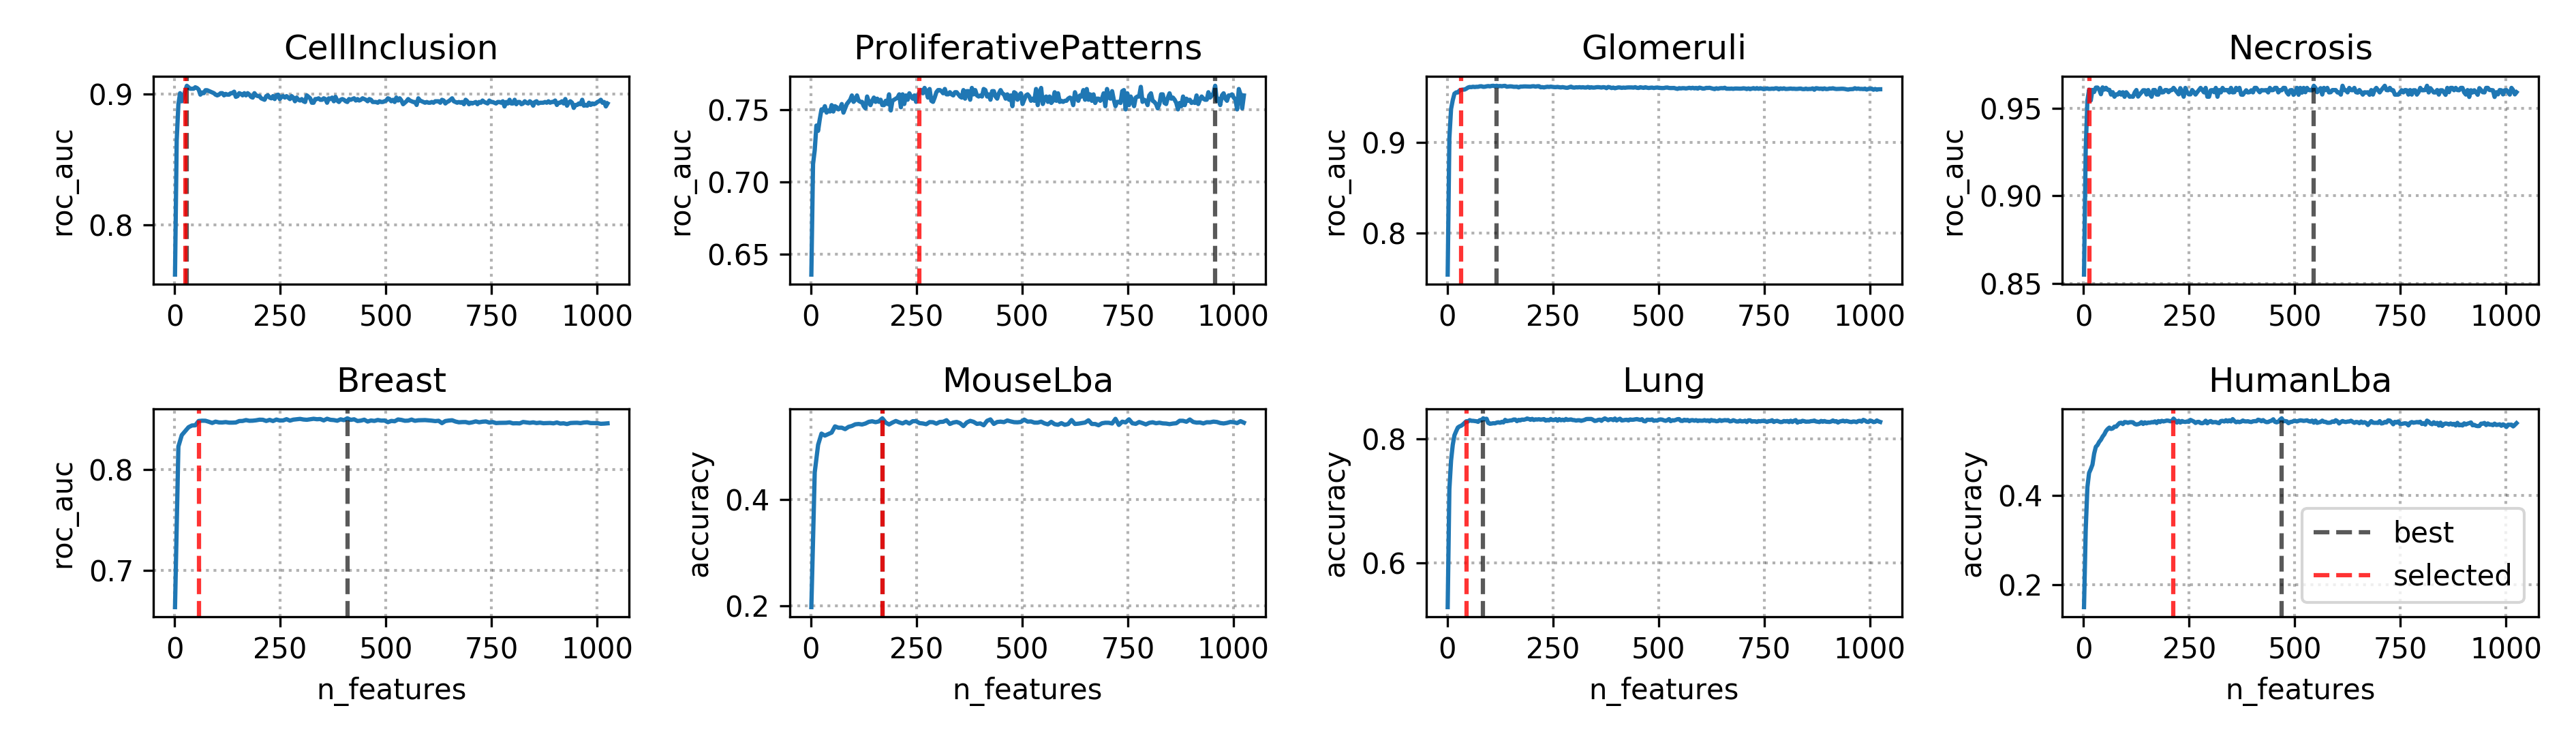
\includegraphics[width=\textwidth]{comp/supp/rfe_mobile.png} \\
    \caption{Mobile}
  \end{subfigure}
  \begin{subfigure}[t]{0.95\textwidth}
    \centering
    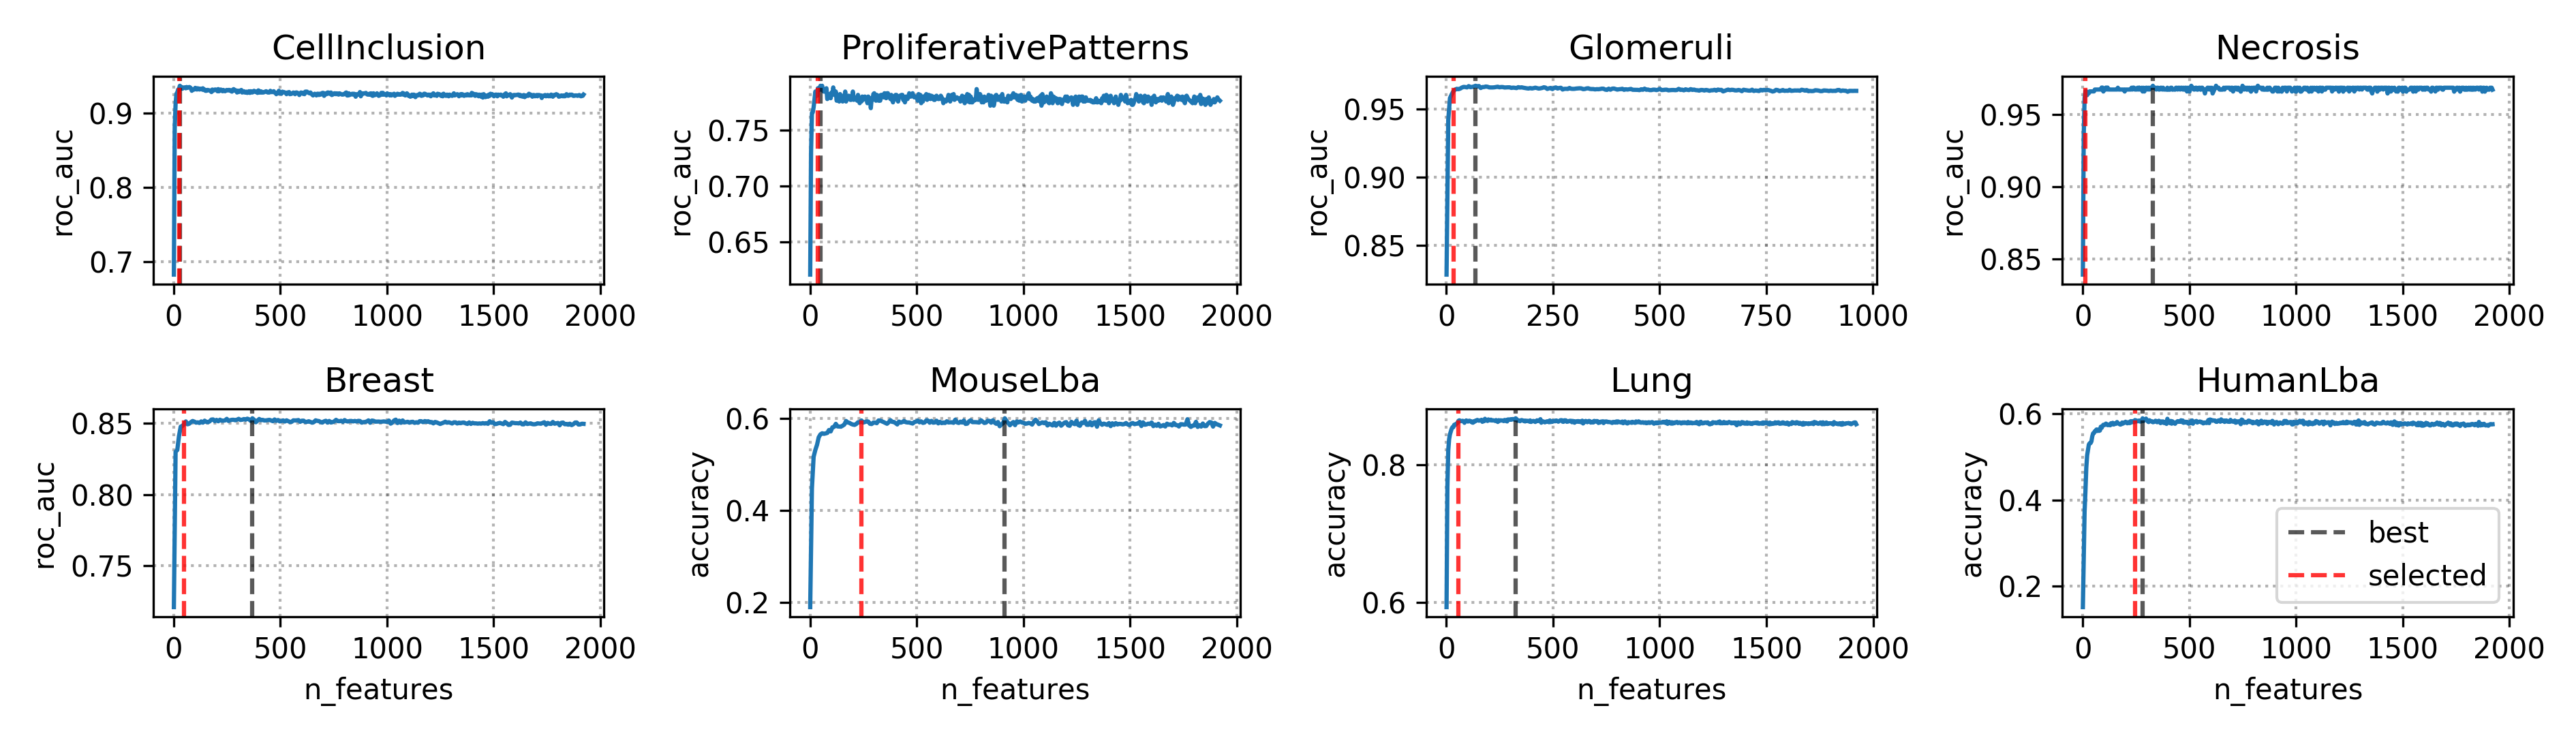
\includegraphics[width=\textwidth]{comp/supp/rfe_dense_net_201.png} \\
    \caption{DenseNet}
  \end{subfigure}
  \begin{subfigure}[t]{0.95\textwidth}
    \centering
    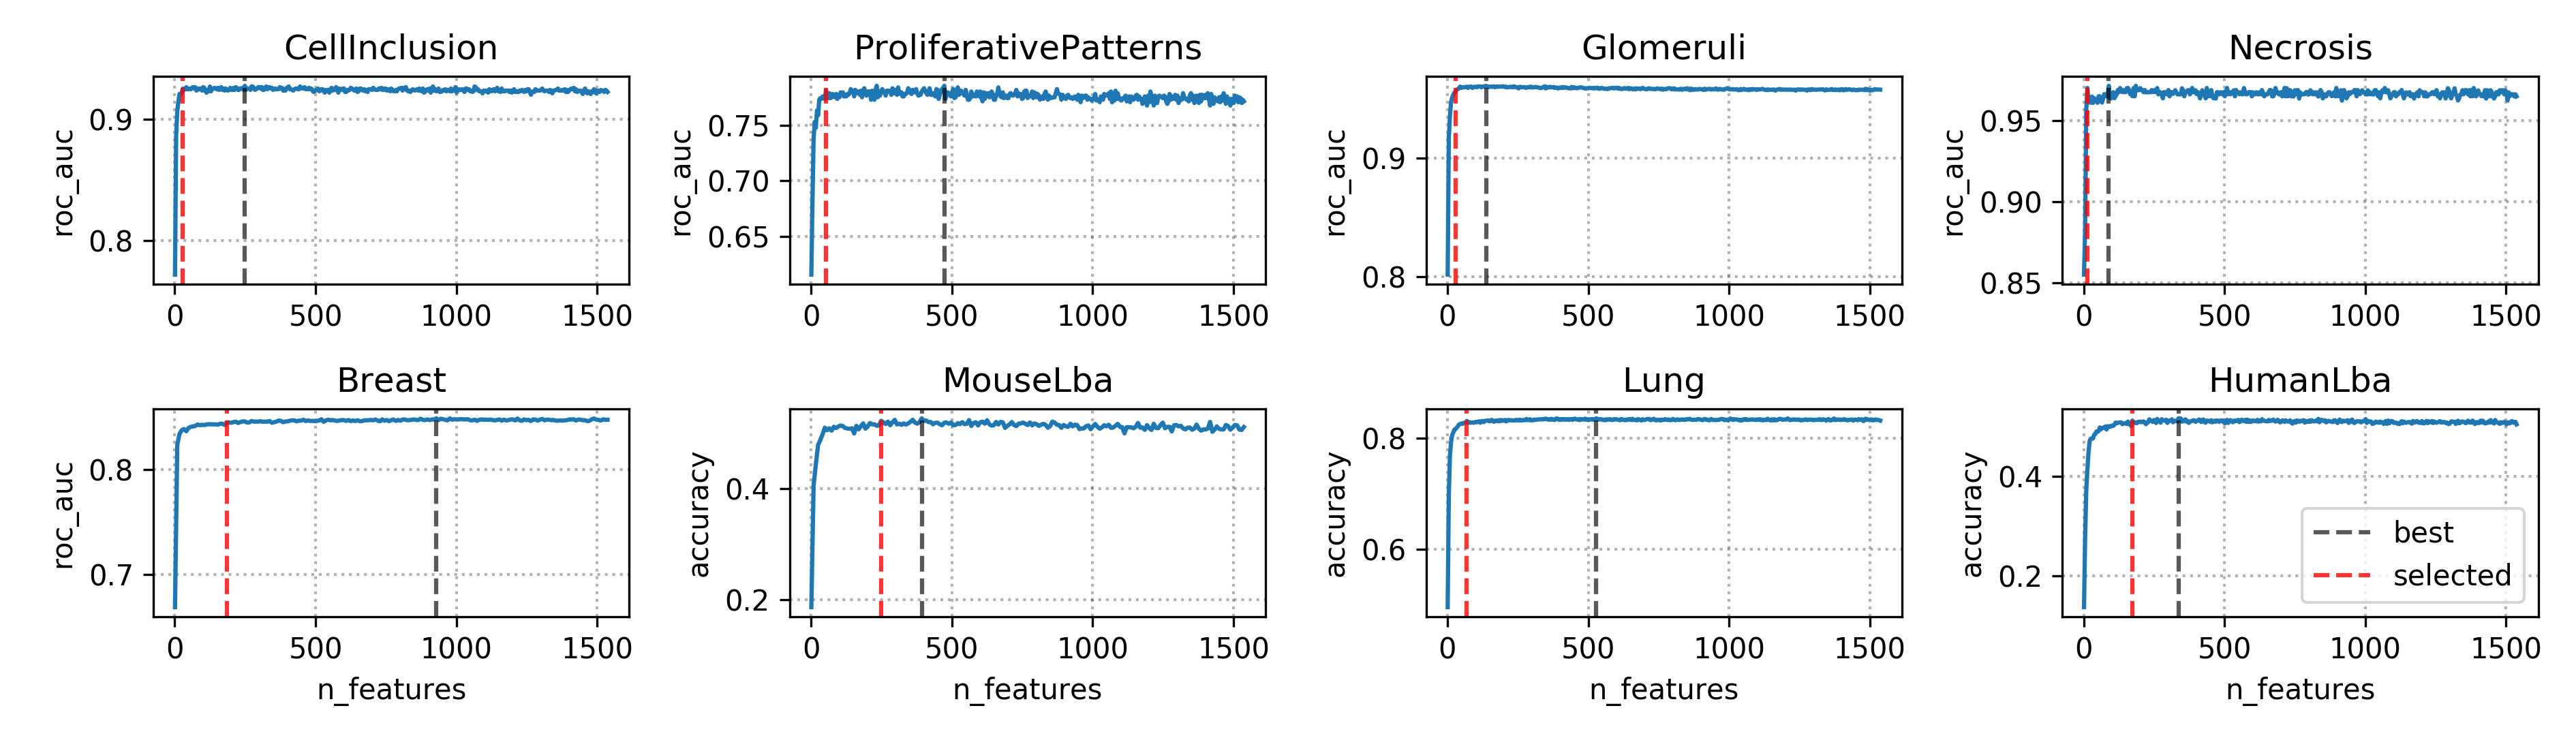
\includegraphics[width=\textwidth]{comp/supp/rfe_inception_resnet_v2.png} \\
    \caption{IncResV2}
  \end{subfigure}
    \begin{subfigure}[t]{0.95\textwidth}
    \centering
    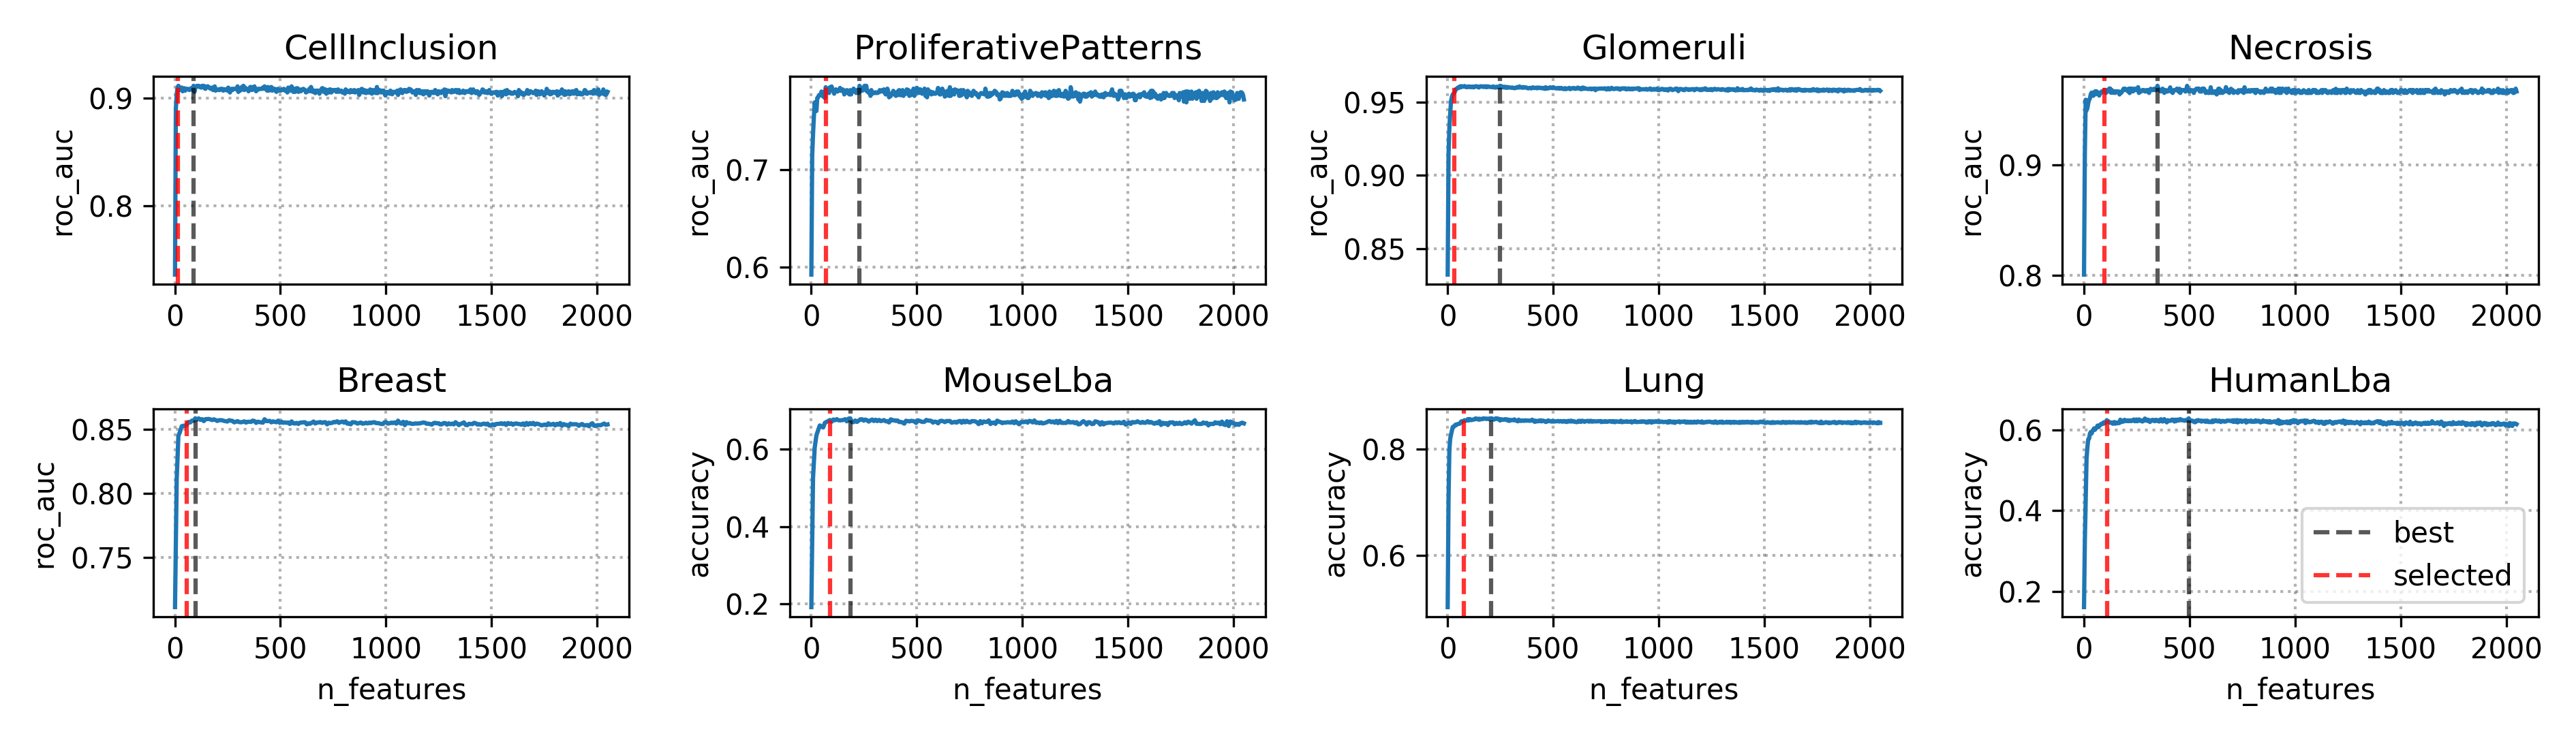
\includegraphics[width=\textwidth]{comp/supp/rfe_resnet50.png}
    \caption{ResNet}
  \end{subfigure}
  \caption{RFE curves for last layers features from InceptionV3, VGG19 and VGG16.}
  \label{app:comp:fig:rfe_1}
\end{figure}

\begin{figure}
	\centering
  \begin{subfigure}[t]{0.99\textwidth}
    \centering
    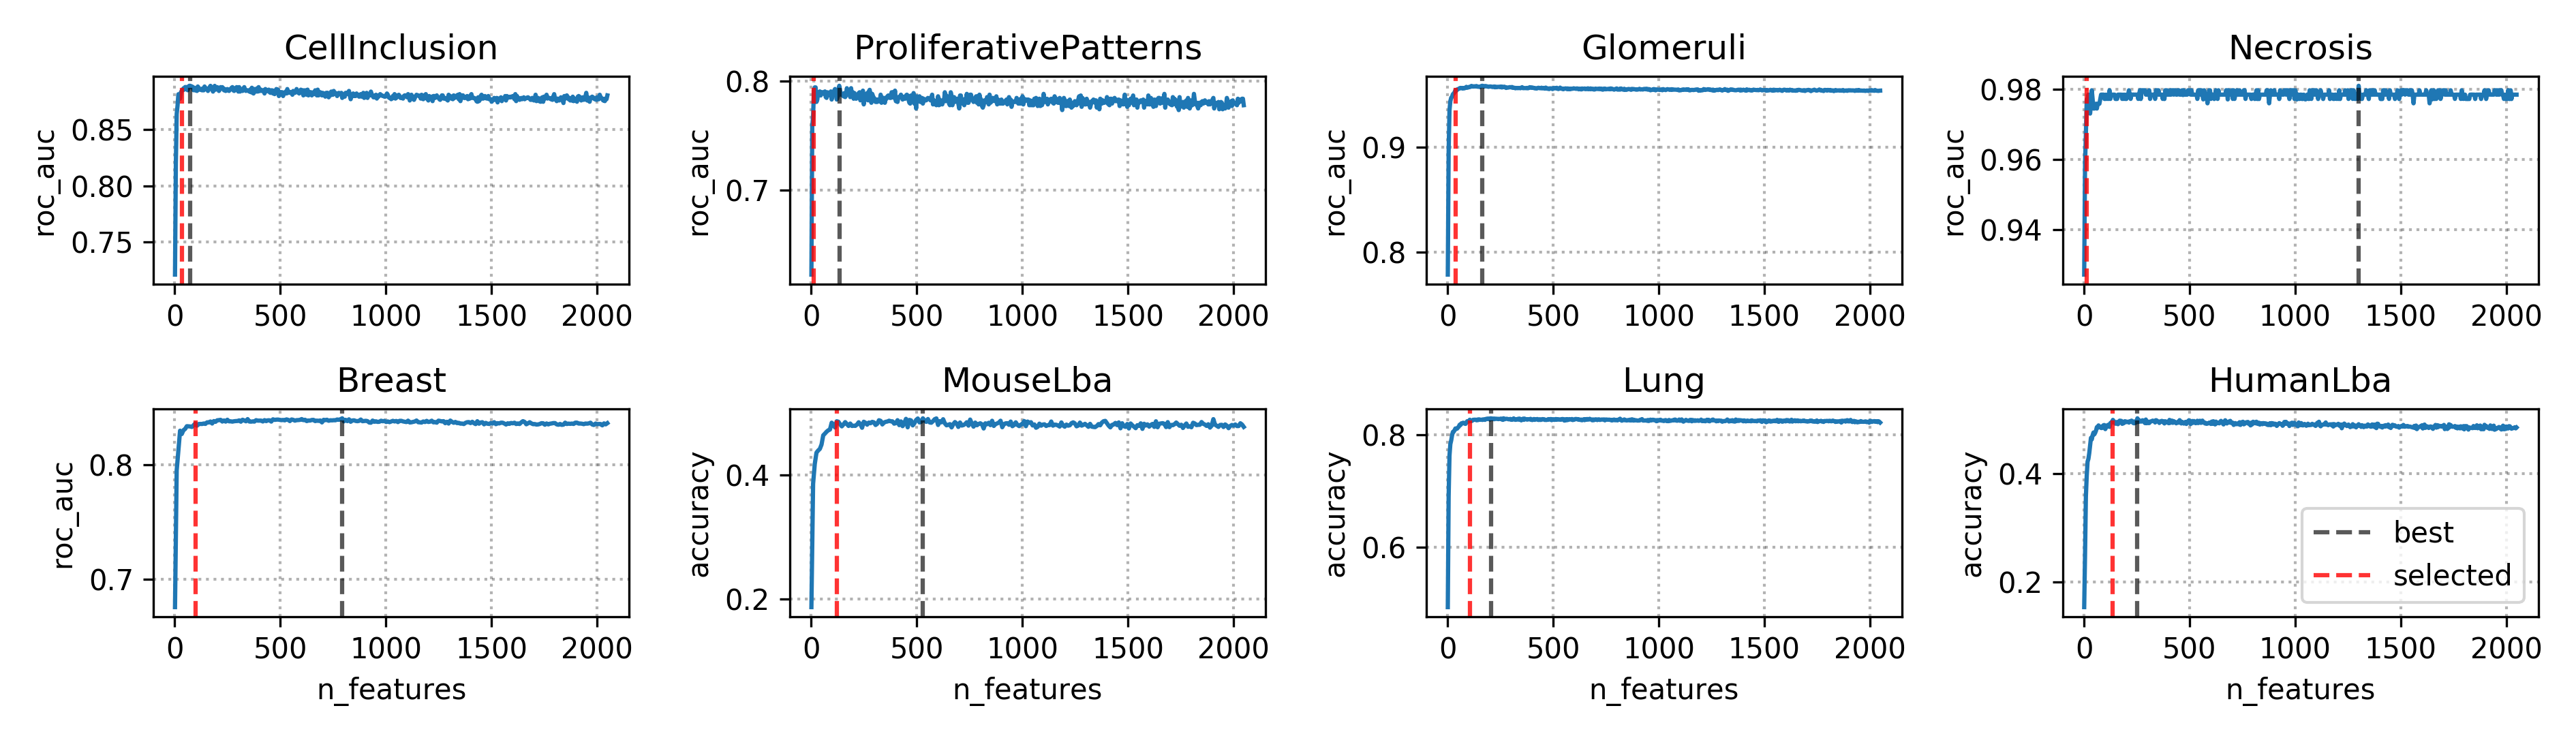
\includegraphics[width=\textwidth]{comp/supp/rfe_inception_v3.png} \\
    \caption{IncV3}
  \end{subfigure}
  \begin{subfigure}[t]{0.99\textwidth}
    \centering
    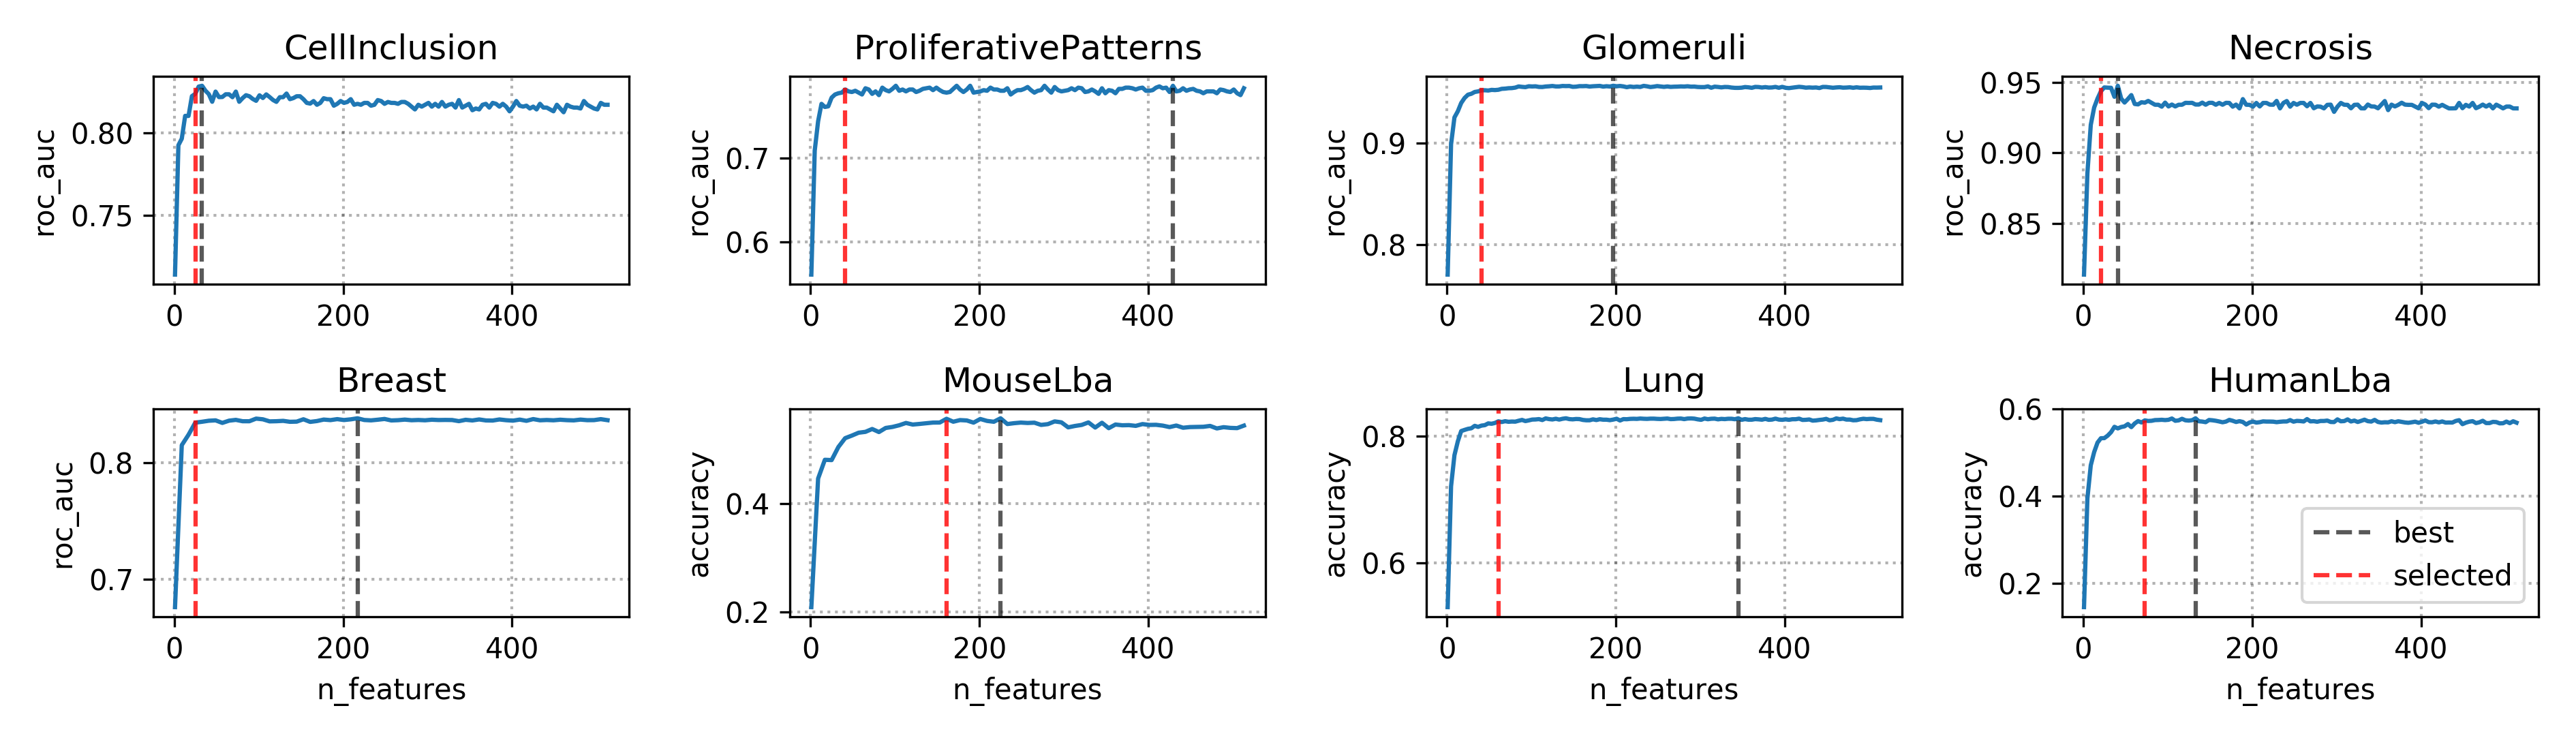
\includegraphics[width=\textwidth]{comp/supp/rfe_vgg19.png} \\
    \caption{VGG19}
  \end{subfigure}
  \begin{subfigure}[t]{0.99\textwidth}
    \centering
    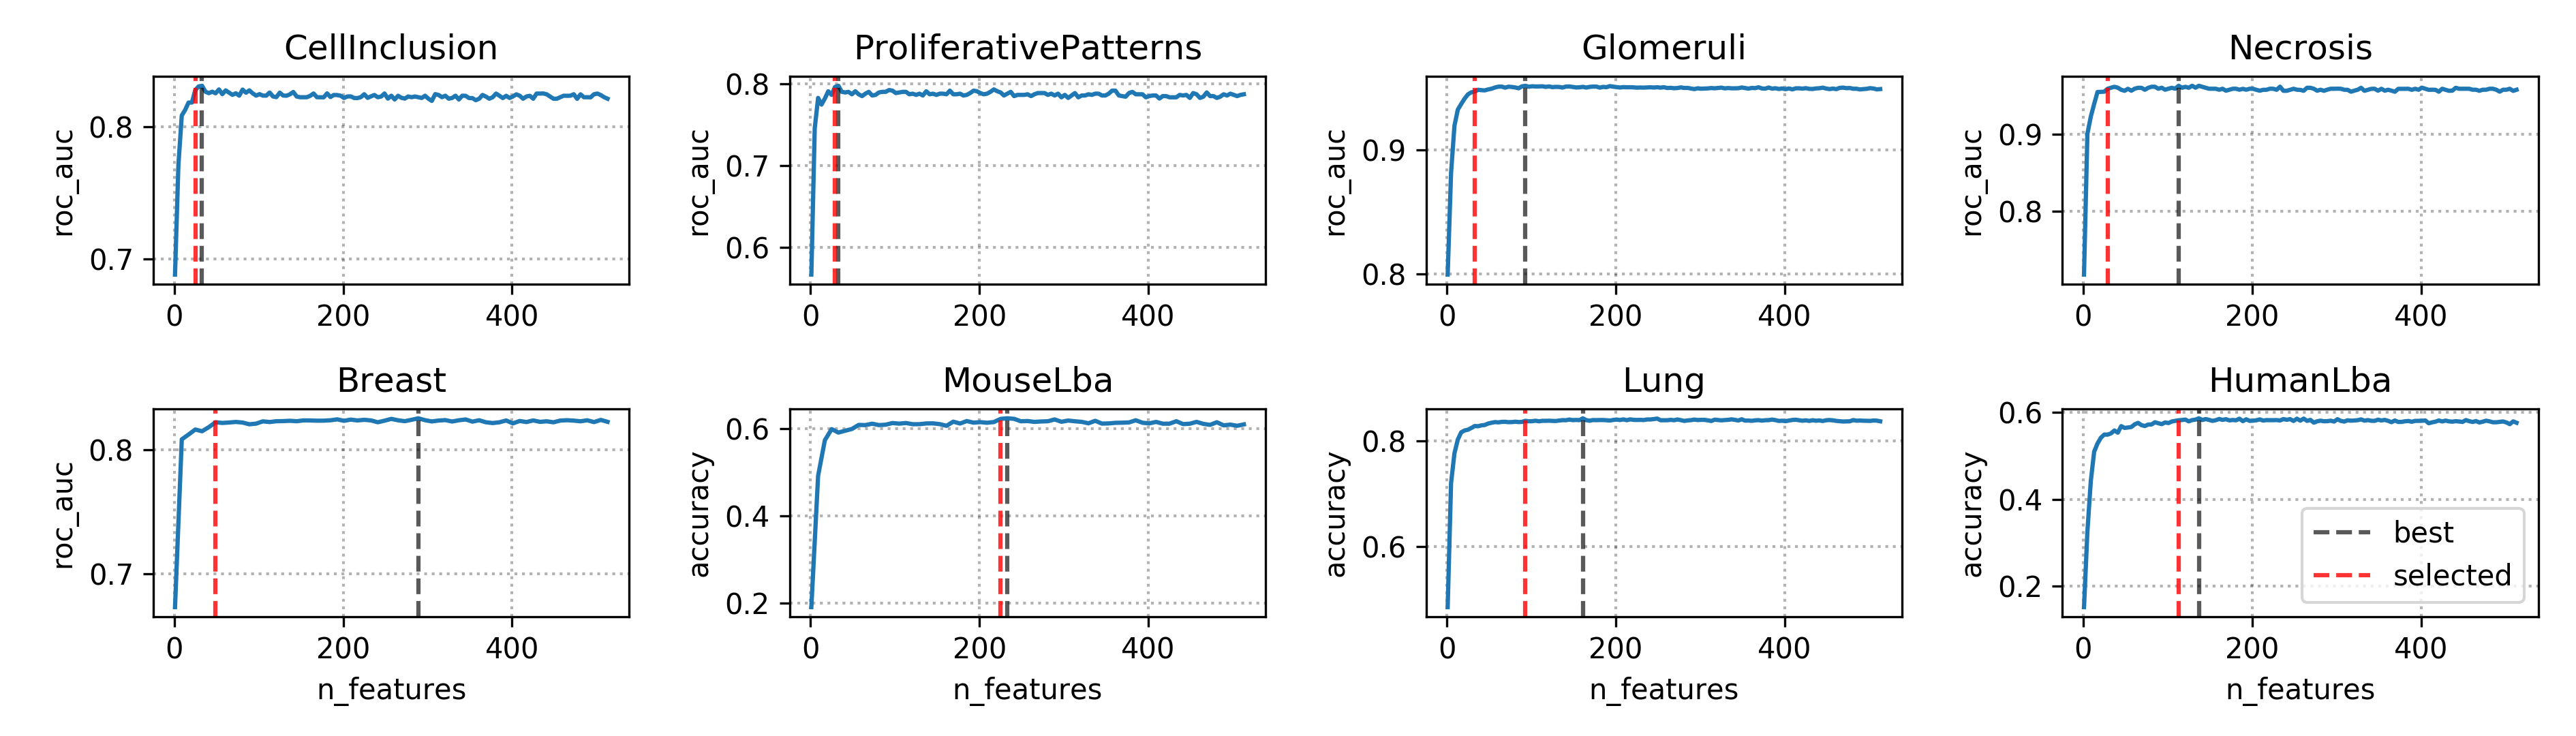
\includegraphics[width=\textwidth]{comp/supp/rfe_vgg16.png} \\
    \caption{VGG16}
  \end{subfigure}
  \caption{Cross validation curves from \acrlong{rfe} for last layers features from InceptionV3, VGG19 and VGG16.}
  \label{app:comp:fig:rfe_2}
\end{figure}

\begin{table}
  \centering
  \small
  \begin{subtable}[h]{0.45\textwidth}
    \centering
    \begin{tabular}{|c|cccccccc|} 
    \hline
    Dataset & \textbf{C} & \textbf{P} & \textbf{G} & \textbf{N} & \textbf{B} & \textbf{M} & \textbf{L} & \textbf{H}\\
    \hline
    \textbf{C} &   & 1 & 3 & 0 & 0 & 3 & 4 & 2 \\
    \textbf{P} & 20 &   & 27 & 53 & 40 & 33 & 33 & 34 \\
    \textbf{G} & 4 & 3 &   & 7 & 14 & 4 & 15 & 6 \\
    \textbf{N} & 0 & 2 & 3 &   & 5 & 1 & 4 & 0 \\
    \textbf{B} & 0 & 8 & 24 & 23 &   & 5 & 17 & 8 \\
    \textbf{M} & 24 & 22 & 21 & 15 & 17 &   & 26 & 31 \\
    \textbf{L} & 8 & 5 & 21 & 15 & 14 & 7 &   & 6 \\
    \textbf{H} & 20 & 28 & 39 & 15 & 33 & 40 & 31 & \\
    \hline
    \end{tabular}
    \caption{Mobile}
  \end{subtable}

  \begin{subtable}[h]{0.45\textwidth}
    \centering
    \begin{tabular}{|c|cccccccc|} 
    \hline
    Dataset & \textbf{C} & \textbf{P} & \textbf{G} & \textbf{N} & \textbf{B} & \textbf{M} & \textbf{L} & \textbf{H}\\
    \hline
    \textbf{C} &   & 1 & 0 & 0 & 3 & 2 & 7 & 3 \\
    \textbf{P} & 3 &   & 3 & 0 & 6 & 4 & 2 & 5 \\
    \textbf{G} & 0 & 1 &   & 0 & 1 & 2 & 0 & 1 \\
    \textbf{N} & 0 & 0 & 0 &   & 0 & 0 & 0 & 0 \\
    \textbf{B} & 20 & 22 & 10 & 7 &   & 14 & 20 & 13 \\
    \textbf{M} & 17 & 22 & 17 & 15 & 18 &   & 20 & 21 \\
    \textbf{L} & 17 & 3 & 0 & 0 & 7 & 5 &   & 7 \\
    \textbf{H} & 20 & 17 & 10 & 0 & 12 & 14 & 18 & \\
    \hline
    \end{tabular}
    \caption{IncResV2}
  \end{subtable} \\

  \begin{subtable}[h]{0.45\textwidth}
    \centering
    \begin{tabular}{|c|cccccccc|} 
    \hline
    Dataset & \textbf{C} & \textbf{P} & \textbf{G} & \textbf{N} & \textbf{B} & \textbf{M} & \textbf{L} & \textbf{H}\\
    \hline
    \textbf{C} &   & 0 & 2 & 0 & 4 & 2 & 3 & 3 \\
    \textbf{P} & 0 &   & 0 & 7 & 0 & 1 & 2 & 1 \\
    \textbf{G} & 3 & 0 &   & 0 & 8 & 1 & 6 & 0 \\
    \textbf{N} & 0 & 7 & 0 &   & 2 & 2 & 1 & 1 \\
    \textbf{B} & 12 & 0 & 21 & 15 &   & 10 & 13 & 10 \\
    \textbf{M} & 9 & 15 & 5 & 23 & 13 &   & 21 & 20 \\
    \textbf{L} & 12 & 23 & 18 & 15 & 14 & 19 &   & 10 \\
    \textbf{H} & 15 & 15 & 2 & 15 & 15 & 23 & 14 & \\
    \hline
    \end{tabular}
    \caption{IncV3}
  \end{subtable}

  \begin{subtable}[h]{0.45\textwidth}
    \centering
    \begin{tabular}{|c|cccccccc|} 
    \hline
    Dataset & \textbf{C} & \textbf{P} & \textbf{G} & \textbf{N} & \textbf{B} & \textbf{M} & \textbf{L} & \textbf{H}\\
    \hline
    \textbf{C} &   & 2 & 0 & 2 & 3 & 3 & 0 & 2 \\
    \textbf{P} & 15 &   & 0 & 7 & 7 & 7 & 14 & 11 \\
    \textbf{G} & 0 & 0 &   & 2 & 5 & 2 & 5 & 1 \\
    \textbf{N} & 15 & 10 & 6 &   & 19 & 11 & 11 & 9 \\
    \textbf{B} & 15 & 5 & 9 & 11 &   & 6 & 16 & 11 \\
    \textbf{M} & 23 & 10 & 6 & 10 & 10 &   & 10 & 23 \\
    \textbf{L} & 0 & 15 & 12 & 9 & 22 & 9 &   & 10 \\
    \textbf{H} & 23 & 18 & 6 & 10 & 21 & 29 & 14 & \\
    \hline
    \end{tabular}
    \caption{ResNet}
  \end{subtable} \\

  \caption{Percentages of overlap between features selected by RFE on the studied datasets (part 1, see Figure \ref{app:comp:tab:rfe_sub_overlap2} for part 2). The tables can be read as follows: the number at row $i$ and column $j$ is the percentage of features among the ones selected for dataset $j$ that were also selected for the dataset $i$.}
  \label{app:comp:tab:rfe_sub_overlap}
\end{table}

\begin{table}
  \centering
  \begin{subtable}[h]{0.45\textwidth}
    \centering
    \begin{tabular}{|c|cccccccc|} 
    \hline
    Dataset & \textbf{C} & \textbf{P} & \textbf{G} & \textbf{N} & \textbf{B} & \textbf{M} & \textbf{L} & \textbf{H}\\
    \hline
    \textbf{C} &   & 10 & 3 & 10 & 8 & 6 & 5 & 7 \\
    \textbf{P} & 12 &   & 9 & 13 & 14 & 9 & 14 & 9 \\
    \textbf{G} & 4 & 10 &   & 13 & 12 & 8 & 17 & 6 \\
    \textbf{N} & 12 & 13 & 12 &   & 16 & 7 & 8 & 11 \\
    \textbf{B} & 16 & 24 & 18 & 27 &   & 16 & 18 & 19 \\
    \textbf{M} & 60 & 72 & 60 & 58 & 73 &   & 62 & 78 \\
    \textbf{L} & 20 & 44 & 48 & 27 & 34 & 25 &   & 26 \\
    \textbf{H} & 32 & 37 & 21 & 44 & 44 & 39 & 32 & \\
    \hline
    \end{tabular}
    \caption{VGG16}
  \end{subtable}

  \begin{subtable}[h]{0.45\textwidth}
    \centering
    \begin{tabular}{|c|cccccccc|} 
    \hline
    Dataset & \textbf{C} & \textbf{P} & \textbf{G} & \textbf{N} & \textbf{B} & \textbf{M} & \textbf{L} & \textbf{H}\\
    \hline
    \textbf{C} &   & 4 & 2 & 4 & 12 & 6 & 8 & 8 \\
    \textbf{P} & 8 &   & 14 & 19 & 12 & 11 & 14 & 16 \\
    \textbf{G} & 4 & 14 &   & 0 & 24 & 10 & 21 & 6 \\
    \textbf{N} & 4 & 9 & 0 &   & 20 & 6 & 9 & 8 \\
    \textbf{B} & 12 & 7 & 14 & 23 &   & 7 & 13 & 9 \\
    \textbf{M} & 44 & 46 & 41 & 52 & 48 &   & 50 & 45 \\
    \textbf{L} & 20 & 22 & 31 & 28 & 32 & 19 &   & 16 \\
    \textbf{H} & 24 & 29 & 12 & 28 & 28 & 20 & 19 & \\
    \hline
    \end{tabular}
    \caption{VGG19}
  \end{subtable} \\

  \begin{subtable}[h]{0.45\textwidth}
    \centering
    \begin{tabular}{|c|cccccccc|} 
    \hline
    Dataset & \textbf{C} & \textbf{P} & \textbf{G} & \textbf{N} & \textbf{B} & \textbf{M} & \textbf{L} & \textbf{H}\\
    \hline
    \textbf{C} &   & 2 & 0 & 0 & 0 & 1 & 3 & 2 \\
    \textbf{P} & 4 &   & 11 & 0 & 2 & 3 & 3 & 3 \\
    \textbf{G} & 0 & 5 &   & 0 & 6 & 0 & 1 & 0 \\
    \textbf{N} & 0 & 0 & 0 &   & 0 & 1 & 0 & 0 \\
    \textbf{B} & 0 & 2 & 17 & 0 &   & 3 & 5 & 2 \\
    \textbf{M} & 16 & 21 & 11 & 23 & 16 &   & 21 & 24 \\
    \textbf{L} & 8 & 5 & 5 & 0 & 6 & 5 &   & 7 \\
    \textbf{H} & 28 & 21 & 11 & 15 & 12 & 24 & 31 & \\
    \hline
    \end{tabular}
    \caption{DenseNet}
  \end{subtable}

  \caption{Percentages of overlap between features selected by RFE on the studied datasets (part 2, see Figure \ref{app:comp:tab:rfe_sub_overlap} for part 1).}
  \label{app:comp:tab:rfe_sub_overlap2}
\end{table}


\begin{table}
  \centering
  \scriptsize
	\begin{tabular}{|c|c|c|ccccc|ccc|}
    \hline
    \textbf{Experiment} & $\mathcal{C}$ & $\mathcal{N}$ & \textbf{C} & \textbf{P} & \textbf{G} & \textbf{N} & \textbf{B} & \textbf{M} & \textbf{L} & \textbf{H} \\
    \hline
    Baseline & \multicolumn{2}{c|}{ET-FL} & 0.9250 & 0.8268 & 0.9551 & 0.9805 & 0.9345 & 0.7568 & 0.8547 & 0.6960 \\
    \hline
    \multirow{8}{*}{Last layer} & \multirow{8}{*}{SVM} & Mobile & 0.9749 & 0.8844 & 0.9935 & 0.9953 & 0.9427 & 0.7611 & 0.9043 & 0.6882 \\
    & & DenseNet & 0.9794 & 0.8852 & 0.9938 & 0.9864 & 0.9257 & 0.7010 & 0.9133 & 0.7820 \\
    & & IncResV2 & 0.9795 & 0.8698 & 0.9928 & 0.9982 & 0.9485 & 0.6566 & 0.9077 & 0.7351 \\
    & & ResNet & 0.9748 & 0.8893 & 0.9924 & 0.9882 & 0.9372 & 0.7633 & 0.9122 & 0.7791 \\
    & & IncV3 & 0.9722 & 0.8670 & 0.9910 & 0.9964 & 0.8951 & 0.6371 & 0.9088 & 0.7175 \\
    & & VGG19 & 0.8853 & 0.8654 & 0.9860 & 0.9905 & 0.9241 & 0.7237 & 0.8885 & 0.7302 \\
    & & VGG16 & 0.8824 & 0.8808 & 0.9859 & 0.9893 & 0.9413 & 0.7438 & 0.9020 & 0.7028 \\
    \hline
    \multirow{8}{*}{Last layer} & \multirow{8}{*}{ET} & Mobile & 0.9608 & 0.8848 & 0.9854 & 0.9840 & 0.9487 & 0.5872 & 0.8648 & 0.7126 \\
    & & DenseNet & 0.9726 & 0.8889 & 0.9891 & 0.9870 & 0.9556 & 0.6381 & 0.8874 & 0.7410 \\
    & & IncResV2 & 0.9618 & 0.8699 & 0.9824 & 0.9953 & 0.9408 & 0.4789 & 0.8570 & 0.6676 \\
    & & ResNet & 0.9634 & 0.8832 & 0.9758 & 0.9929 & 0.9507 & 0.6186 & 0.8851 & 0.7752 \\
    & & IncV3 & 0.9481 & 0.8795 & 0.9793 & 0.9929 & 0.9428 & 0.4583 & 0.8300 & 0.6305 \\
    & & VGG19 & 0.8551 & 0.8430 & 0.9795 & 0.9861 & 0.9231 & 0.5379 & 0.8536 & 0.6989 \\
    & & VGG16 & 0.8412 & 0.8791 & 0.9690 & 0.9888 & 0.9254 & 0.5791 & 0.8659 & 0.6833 \\
    \hline
    \multirow{8}{*}{Last layer} & \multirow{8}{*}{FC} & Mobile & 0.9796 & 0.8661 & 0.9794 & 0.9935 & 0.9603 & 0.7941 & 0.8986 & 0.6823 \\
    & & DenseNet & 0.9822 & 0.8668 & 0.8316 & 0.9852 & 0.9482 & 0.7291 & 0.9054 & 0.7664 \\
    & & IncResV2 & 0.9756 & 0.8676 & 0.9729 & 0.9976 & 0.9597 & 0.6598 & 0.9043 & 0.7038 \\
    & & ResNet & 0.9726 & 0.8670 & 0.9771 & 0.9899 & 0.9583 & 0.7996 & 0.9133 & 0.7674 \\
    & & IncV3 & 0.9714 & 0.8417 & 0.9796 & 0.9893 & 0.9377 & 0.6538 & 0.8998 & 0.7038 \\
    & & VGG19 & 0.8447 & 0.8553 & 0.9661 & 0.9899 & 0.9237 & 0.6636 & 0.8863 & 0.7410 \\
    & & VGG16 & 0.8298 & 0.8718 & 0.9573 & 0.9852 & 0.9421 & 0.6956 & 0.9088 & 0.7185 \\
    \hline
    \multirow{8}{*}{Feature selection} & \multirow{8}{*}{SVM} & Mobile & 0.9610 & 0.7876 & 0.9794 & 0.9870 & 0.9597 & 0.7421 & 0.8682 & 0.6618 \\
    & & DenseNet & 0.9347 & 0.8212 & 0.8316 & 0.9888 & 0.9436 & 0.6614 & 0.7984 & 0.6931 \\
    & & IncResV2 & 0.9665 & 0.8476 & 0.9729 & 0.9976 & 0.9443 & 0.6403 & 0.8682 & 0.7214 \\
    & & ResNet & 0.9578 & 0.8337 & 0.9771 & 0.9722 & 0.9492 & 0.7438 & 0.8806 & 0.7644 \\
    & & IncV3 & 0.9562 & 0.8308 & 0.9796 & 0.9964 & 0.9436 & 0.6430 & 0.8750 & 0.6843 \\
    & & VGG19 & 0.8284 & 0.8488 & 0.9661 & 0.9888 & 0.8860 & 0.6750 & 0.8784 & 0.7038 \\
    & & VGG16 & 0.8071 & 0.8810 & 0.9573 & 0.9899 & 0.9131 & 0.7362 & 0.8941 & 0.7038 \\
    \hline
    \multirow{8}{*}{Feature selection} & \multirow{8}{*}{ET} & Mobile & 0.9617 & 0.8798 & 0.9799 & 0.9888 & 0.9581 & 0.6582 & 0.8694 & 0.7400 \\
    & & DenseNet & 0.9676 & 0.8861 & 0.9843 & 0.9994 & 0.9489 & 0.6939 & 0.8919 & 0.6667 \\
    & & IncResV2 & 0.9609 & 0.8646 & 0.9743 & 0.9944 & 0.9421 & 0.5330 & 0.8491 & 0.6500 \\
    & & ResNet & 0.9503 & 0.8786 & 0.9799 & 0.9852 & 0.9488 & 0.6961 & 0.8863 & 0.7038 \\
    & & IncV3 & 0.9473 & 0.8410 & 0.9786 & 0.9959 & 0.9466 & 0.5531 & 0.8378 & 0.7703 \\
    & & VGG19 & 0.8506 & 0.8492 & 0.9732 & 0.9947 & 0.9186 & 0.5850 & 0.8468 & 0.7019 \\
    & & VGG16 & 0.8232 & 0.8774 & 0.9659 & 0.9953 & 0.9282 & 0.6349 & 0.8615 & 0.6745 \\
    \hline
    \multirow{2}{*}{Merging networks} & ET & merged & 0.9897 & 0.8573 & 0.9948 & 0.9858 & 0.8851 & 0.8169 & 0.9155 & 0.7928 \\
    & SVM & merged & 0.9784 & 0.8984 & 0.9912 & 0.9864 & 0.9549 & 0.6896 & 0.8615 & 0.6063 \\
    \hline
    \multirow{4}{*}{Merging layers} & \multirow{4}{*}{SVM} & DenseNet & 0.9757 & 0.8090 & 0.9835 & 0.9870 & 0.9470 & 0.7042 & 0.8840 & 0.7761 \\
    & & IncResV2 & 0.9808 & 0.8418 & 0.9920 & 0.9964 & 0.9559 & 0.7031 & 0.9155 & 0.7761 \\
    & & ResNet & 0.9789 & 0.8576 & 0.9927 & 0.9953 & 0.9234 & 0.7941 & 0.9268 & 0.7977 \\
    \hline
    \multirow{4}{*}{Merging layers} & \multirow{4}{*}{ET} & DenseNet & 0.9605 & 0.8892 & 0.9875 & 0.9911 & 0.9588 & 0.6993 & 0.8818 & 0.7370 \\
    & & IncResV2 & 0.9799 & 0.8906 & 0.9944 & 0.9920 & 0.9639 & 0.6495 & 0.8897 & 0.7370 \\
    & & ResNet & 0.9424 & 0.8787 & 0.9847 & 0.9929 & 0.9619 & 0.7080 & 0.8885 & 0.7683 \\
    \hline
    \multirow{3}{*}{Fine-tuning} & \multirow{3}{*}{SVM} & DenseNet & 0.9883 & 0.8556 & 0.9944 & 0.9870 & 0.9777 & 0.8342 & 0.9119 & 0.8553 \\
    & & IncResV2 & 0.9841 & 0.8377 & 0.9909 & 0.9941 & 0.9403 & 0.6847 & 0.9039 & 0.7390 \\
    & & ResNet & 0.9921 & 0.8705 & 0.9897 & 0.9941 & 0.9637 & 0.8147 & 0.9119 & 0.8456 \\
    \hline
    \multirow{3}{*}{Fine-tuning} & \multirow{3}{*}{ET} & DenseNet & 0.9828 & 0.8965 & 0.9950 & 0.9876 & 0.9827 & 0.7887 & 0.8982 & 0.8094 \\
    & & IncResV2 & 0.9769 & 0.8776 & 0.9850 & 0.9929 & 0.9477 & 0.5406 & 0.8446 & 0.7048 \\
    & & ResNet & 0.9909 & 0.8806 & 0.9879 & 0.9870 & 0.9772 & 0.7763 & 0.8845 & 0.8289 \\
    \hline
    \multirow{3}{*}{Fine-tuning} & \multirow{3}{*}{Net} & DenseNet & 0.9892 & 0.8797 & 0.9977 & 0.9893 & 0.9835 & 0.8483 & 0.9405 & 0.8641 \\
    & & IncResV2 & 0.9851 & 0.8795 & 0.9971 & 0.9929 & 0.9873 & 0.8727 & 0.9165 & 0.8182 \\
    & & ResNet & 0.9926 & 0.8778 & 0.9953 & 0.9970 & 0.9827 & 0.8288 & 0.8971 & 0.8416 \\
    \hline
    \multicolumn{3}{|c|}{\textbf{Metric}} & \multicolumn{5}{c|}{ROC AUC} & \multicolumn{3}{c|}{Accuracy (multi-class)} \\
    \hline
  \end{tabular}
  \caption{Detailed scores for all datasets and for the ``\textit{Last layer}'', ``\textit{Feature selection}'', ``\textit{Merging features across networks}'', ``\textit{Merging features across layers}'' and ``\textit{Fine-tuning}'' experiments.}
  \label{app:comp:tab:detailed_first}
\end{table}

\begin{table}
  \centering
  \scriptsize
  \begin{tabular}{|c|c|ccccc|ccc|}
    \hline
    $\mathcal{N}$ & \textbf{Layer $l$}  & \textbf{C} & \textbf{P} & \textbf{G} & \textbf{N} & \textbf{B} & \textbf{M} & \textbf{L} & \textbf{H} \\
    \hline
    \multicolumn{2}{|c|}{Baseline / ET-FL} & 0.9250 & 0.8268 & 0.9551 & 0.9805 & 0.9345 & 0.7568 & 0.8547 & 0.6960 \\
    \hline
    \multirow{17}{*}{ResNet} & activation\_1 & 0.7720 & 0.8415 & 0.9275 & 0.9811 & 0.9100 & 0.4946 & 0.8153 & 0.5758 \\
    & activation\_4 & 0.8283 & 0.8275 & 0.9723 & 0.9964 & 0.9390 & 0.7308 & 0.8806 & 0.6285 \\
    & activation\_7 & 0.8456 & 0.8276 & 0.9772 & 0.9888 & 0.9351 & 0.7275 & 0.8930 & 0.6755 \\
    & activation\_10 & 0.8574 & 0.8292 & 0.9759 & 0.9882 & 0.9439 & 0.6717 & 0.8930 & 0.6491 \\
    & activation\_13 & 0.8859 & 0.8608 & 0.9824 & 0.9888 & 0.9483 & 0.7313 & 0.9077 & 0.6188 \\
    & activation\_16 & 0.8975 & 0.8418 & 0.9860 & 0.9876 & 0.9478 & 0.7356 & 0.9054 & 0.6598 \\
    & activation\_19 & 0.8877 & 0.8503 & 0.9892 & 0.9888 & 0.9499 & 0.7270 & 0.9077 & 0.6510 \\
    & activation\_22 & 0.9244 & 0.8763 & 0.9892 & 0.9882 & 0.9555 & 0.7010 & 0.9223 & 0.6940 \\
    & activation\_25 & 0.9506 & 0.8785 & 0.9933 & 0.9858 & 0.9639 & 0.7736 & 0.9223 & 0.7253 \\
    & activation\_28 & 0.9489 & 0.8884 & 0.9935 & 0.9876 & 0.9638 & 0.8131 & 0.9245 & 0.7634 \\
    & activation\_31 & 0.9519 & 0.8724 & 0.9938 & 0.9876 & 0.9659 & 0.7996 & 0.9201 & 0.7351 \\
    & activation\_34 & 0.9584 & 0.8947 & 0.9940 & 0.9876 & 0.9606 & 0.7514 & 0.9223 & 0.7977 \\
    & activation\_37 & 0.9671 & 0.8959 & 0.9942 & 0.9876 & 0.9663 & 0.7600 & 0.9280 & 0.7996 \\
    & activation\_40 & 0.9621 & 0.8894 & 0.9949 & 0.9864 & 0.9664 & 0.7914 & 0.9155 & 0.8113 \\
    & activation\_43 & 0.9710 & 0.8950 & 0.9942 & 0.9852 & 0.9648 & 0.8017 & 0.9223 & 0.8074 \\
    & activation\_46 & 0.9712 & 0.8848 & 0.9937 & 0.9870 & 0.9652 & 0.7860 & 0.9291 & 0.8094 \\
    & activation\_49 (last) & 0.9748 & 0.8893 & 0.9924 & 0.9882 & 0.9640 & 0.7860 & 0.9122 & 0.7791 \\
    \hline
    \multirow{11}{*}{DenseNet} & pool1 & 0.7187 & 0.8276 & 0.8994 & 0.9533 & 0.9227 & 0.4821 & 0.7826 & 0.4653 \\
    & conv2\_block6\_concat & 0.7982 & 0.8374 & 0.9609 & 0.9905 & 0.9374 & 0.6300 & 0.8536 & 0.5259 \\
    & pool2\_pool & 0.8185 & 0.8296 & 0.9570 & 0.9893 & 0.9510 & 0.6235 & 0.8570 & 0.5337 \\
    & conv3\_block12\_concat & 0.9024 & 0.8361 & 0.9861 & 0.9882 & 0.9522 & 0.6696 & 0.9020 & 0.6823 \\
    & pool3\_pool & 0.9309 & 0.8900 & 0.9832 & 0.9893 & 0.9382 & 0.6300 & 0.9088 & 0.6686 \\
    & conv4\_block48\_concat & 0.9803 & 0.8876 & 0.9962 & 0.9870 & 0.9699 & 0.8012 & 0.9223 & 0.7674 \\
    & pool4\_pool & 0.9843 & 0.8984 & 0.9954 & 0.9870 & 0.9613 & 0.7703 & 0.9268 & 0.7859 \\
    & conv5\_block32\_concat & 0.9862 & 0.8981 & 0.9955 & 0.9917 & 0.9623 & 0.7806 & 0.9201 & 0.7879 \\
    & bn (last) & 0.9784 & 0.8867 & 0.9931 & 0.9852 & 0.9538 & 0.7573 & 0.9043 & 0.7967 \\
    \hline
    \multirow{18}{*}{IncResV2} & max\_pooling2d\_2 & 0.8403 & 0.8091 & 0.9716 & 0.9941 & 0.9340 & 0.6143 & 0.8851 & 0.6158 \\
    & mixed\_5b & 0.8265 & 0.8146 & 0.9771 & 0.9905 & 0.9424 & 0.6945 & 0.8897 & 0.6461 \\
    & block35\_1\_ac & 0.8325 & 0.8412 & 0.9776 & 0.9941 & 0.9412 & 0.6576 & 0.8897 & 0.6373 \\
    & block35\_4\_ac & 0.8673 & 0.8770 & 0.9834 & 0.9923 & 0.9556 & 0.6495 & 0.8998 & 0.6716 \\
    & block35\_7\_ac & 0.8981 & 0.8709 & 0.9844 & 0.9935 & 0.9590 & 0.6354 & 0.9043 & 0.7048 \\
    & block35\_10\_ac & 0.9219 & 0.8692 & 0.9900 & 0.9935 & 0.9616 & 0.6549 & 0.9110 & 0.7253 \\
    & mixed\_6a & 0.9445 & 0.8747 & 0.9920 & 0.9953 & 0.9706 & 0.7172 & 0.9088 & 0.7439 \\
    & block17\_5\_ac & 0.9681 & 0.8665 & 0.9945 & 0.9917 & 0.9695 & 0.8066 & 0.9190 & 0.7713 \\
    & block17\_10\_ac & 0.9711 & 0.8687 & 0.9958 & 0.9935 & 0.9720 & 0.8137 & 0.9234 & 0.7674 \\
    & block17\_15\_ac & 0.9762 & 0.8939 & 0.9960 & 0.9923 & 0.9622 & 0.7985 & 0.9144 & 0.7419 \\
    & block17\_20\_ac & 0.9860 & 0.8948 & 0.9957 & 0.9923 & 0.9649 & 0.7741 & 0.9155 & 0.7693 \\
    & block8\_3\_ac & 0.9873 & 0.8905 & 0.9959 & 0.9953 & 0.9676 & 0.7790 & 0.9190 & 0.7273 \\
    & block8\_6\_ac & 0.9868 & 0.8871 & 0.9953 & 0.9923 & 0.9686 & 0.7562 & 0.9212 & 0.7468 \\
    & block8\_9\_ac & 0.9824 & 0.8773 & 0.9946 & 0.9964 & 0.9632 & 0.7427 & 0.9144 & 0.7468 \\
    & mixed\_7a & 0.9868 & 0.8934 & 0.9962 & 0.9959 & 0.9602 & 0.7893 & 0.9178 & 0.7214 \\
    & conv\_7b\_ac (last) & 0.9773 & 0.8615 & 0.9926 & 0.9982 & 0.9619 & 0.6766 & 0.8998 & 0.7361 \\
    \hline
    \multicolumn{2}{|c|}{\textbf{Metric}} & \multicolumn{5}{c|}{ROC AUC} & \multicolumn{3}{c|}{Accuracy (multi-class)} \\
    \hline
  \end{tabular}
  \caption{Detailed scores for all datasets and for the ``\textit{Inner layer}'' experiment.}
  \label{app:comp:tab:detailed_second}
\end{table}

\chapter{Appendices for Chapter \ref{chap:mtask}}
\label{app:mtask:app:mtask}

\section{Data preparation}
\label{app:mtask:sec:app:datasets}

The general goal of the pre-processing is to obtain images which dimensions are compatible with state of the art neural networks (\eg ResNet \cite{he2016deep}, DenseNet \cite{huang2017densely}) and that are properly labeled. Classification (CLF) datasets already had classes associated to each image. For these datasets, we have thus kept the original classes. When datasets had large input images, we have further splitted them into smaller patches (see Table \ref{app:mtask:tab:app:details_trans_clf}).

We have considered the detection (DET) datasets to be the ones that contained several objects per input image where each object was usually denoted by a point annotation, and sometimes a label (\eg Warwick CRC \cite{sirinukunwattana2016locality}). For those datasets, the transformations were more involved (see Table \ref{app:mtask:tab:app:details_trans_det}). When the concentration of annotations was high (\ie a typical patch in the image contains tens of annotations) and/or the input image size was small (\ie $<$ 1k pixels square), overlapping patches were extracted. Each patch was associated a binary class indicating whether the entity to detect was present or absent in this patch. When a label was available, the associated class was chosen to indicate the presence of one type of object versus the other(s). For datasets where the objects to detect were fewer and more scattered over the input images (\eg mitosis detection), the previous approach was inappropriate as it would have yielded highly imbalanced datasets. Therefore, in this case, negative patches were still sampled exhaustively with an overlap but positive patches were sampled around the objects of interest with random shifts, yielding several samples per object. 

For the segmentation (SEG) datasets (see Table \ref{app:mtask:tab:app:details_trans_seg}), the patch sampling was the same as for the detection (\ie exhaustive with overlap). The class was determined if the surface ratio of the positive entity (\eg tumor) in the patch exceeded a threshold (\eg 10\% of the patch). The only exception is \textit{Breast1} dataset for which the class of the patch is the class of its central pixel. Camelyon16 \cite{bejnordi2017diagnostic} dataset was applied an additionnal pre-processing to exclude most of the whole-slide image (WSI) background.

The last transformation step was to split each resulting dataset into some training, validation and test sets for future training. We have followed a rigorous splitting process: whenever possible we have made sure that images from a same patient, or a same slide were not in two different sets. Sometimes, none of those information were available in which case we have randomly split the data. Moreover, we have ensured that all classes were present in all sets.

Resulting classification datasets and their splits are listed in Table \ref{app:mtask:tab:app:final_datasets}. Selected samples for each of our final classification tasks are given in Figure \ref{fig:mtask:dataset_samples}.

\begin{table}
\center
\caption{Details for classification datasets transforms. Patches indicate whether the final patches are the \textit{original} images. Provided dimensions indicate that patches of those dimensions were extracted from the original images to make the final classification datasets.}
\label{app:mtask:tab:app:details_trans_clf}
\begin{tabular}{|c|c|c|}
\hline
Dataset & Patches \\
\hline
BACH1018 Micro & 512 $\times$ 512 \\
Stroma LBP & original \\
UMCM Colorectal & original \\
Janowczyk & original \\ 
Janowczyk & 384 $\times$ 384 \\
\hline
\end{tabular}
\end{table}

\begin{table*}[t]
\center
\caption{Details for detection datasets transforms. Columns \textit{Positive} and \textit{negative} indicate which annotation information or label was used to set respectively the patch class as positive or negative. The $\emptyset$ means "\textit{no annotation}". Column "\textit{Supersample}" indicates whether or not the positive patches was supersampled, and if so, how many patches were extracted per positive annotation.  }
\label{app:mtask:tab:app:details_trans_det}
\begin{tabular}{|c|c|c|c|c|c|c|}
\hline
Dataset & Positive & Negative & Other & Dimensions & Overlap & Supersample \\
\hline
Warwick CRC & {\small $\left\{\text{Inflammatory}\right\}$} & {\small $\left\{\text{Epithelial}, \text{Fibroblast}, \text{Others}, \emptyset\right\}$} & / & 100 $\times$ 100 & 0 & / \\
TUPAC2016 Mitosis & {\small $\left\{\text{Mitosis}\right\}$} & {\small $\left\{\emptyset\right\}$} & / & 250 $\times$ 250 & 0 & 10 \\
MITOS-ATYPIA & {\small $\left\{\text{Mitosis}\right\}$} & {\small $\left\{\emptyset\right\}$} & {$\left\{\text{NonMitosis}\right\}$} & 323 $\times$ 323 & 0 & 10 \\
Janowczyk 5 & {\small $\left\{\text{Mitosis}\right\}$} & {\small $\left\{\emptyset\right\}$} & / & 250 $\times$ 250 & 0 & 10 \\
\hline
\end{tabular}
\end{table*}

\begin{table*}[t]
\center
\caption{Details for segmentation datasets transforms. \textit{Area} is the surface threshold we have used to separate positive from negative patches (if surface of positive annotation was larger than the given value, then the patch was considered positive). Column "\textit{WSI}" indicates that the original images are whole-slide images and were applied additional pre-processing to remove background tiles. Column "\textit{P/CW}" indicates whether or not the patches were subsampled. If a value is provided, this value is the maximum number of samples per class per WSI capped that was produced.}
\label{app:mtask:tab:app:details_trans_seg}
\begin{tabular}{|c|c|c|c|c|c|c|c|c|c|c|}
\hline
\multirow{2}{*}{Dataset} & \multicolumn{3}{c}{Classes} & \multicolumn{3}{|c|}{Dimensions} & \multirow{2}{*}{WSI} & \multirow{2}{*}{P/CW} \\
\cline{2-7}
 & Positive & Negative & Area {\small($\%$)} & Extracted & Rescaled & Overlap & & \\
\hline
Janowczyk 1 & {\small $\left\{\text{Nuclei}\right\}$} &  {\small $\left\{\emptyset\right\}$} & 5 & 250 $\times$ 250 & / & 125 & no & / \\
Janowczyk 2 & {\small $\left\{\text{Epithelium}\right\}$} &  {\small $\left\{\emptyset\right\}$} & 10 & 200 $\times$ 200 & / & 100 & no & / \\
Camelyon 16 & {\small $\left\{\text{Tumor}\right\}$} &  {\small $\left\{\emptyset\right\}$} & 10 & 768 $\times$ 768 & 384 $\times$ 384 & 0 & yes & 1000 \\
Breast1 & {\small $\left\{\text{InSitu, Infiltration}\right\}$} & {\small $\left\{\emptyset\right\}$} & / & 384 $\times$ 384 & / & / & no & /\\
Breast2 & {\small $\left\{\text{InSitu, Infiltration}\right\}$} & {\small $\left\{\emptyset\right\}$} & 10 & 250 $\times$ 250 & / & 125 & no & /\\
\hline
\end{tabular}
\end{table*}

\begin{table*}[t]
    \centering
    \caption{Classification datasets generated from the collected datasets. \textit{p/s} indicate the number of distinct patients, or slides (if no patient information was available), or images (in case when none of the two information were available) in the set. The column \textit{Split} indicates whether the dataset was split patient, slide or image-wise.}
    \label{app:mtask:tab:app:final_datasets}
    \begin{tabular}{|c|c|r:r|r:r|r:r|r:r|c|}
\hline
\multirow{2}{*}{\textbf{Name}} & \multirow{2}{*}{\textbf{Cls}} & \multicolumn{2}{c|}{\textbf{Train}} & \multicolumn{2}{c|}{\textbf{Val}} & \multicolumn{2}{c|}{\textbf{Test}} & \multicolumn{2}{c|}{\textbf{Total}} & \multirow{2}{*}{\textbf{Split}} \\
\cline{3-10}
 & &  \multicolumn{1}{c:}{\textbf{Img.}} & \multicolumn{1}{c|}{\textbf{p/s}} & \multicolumn{1}{c:}{\textbf{Img.}} & \multicolumn{1}{c|}{\textbf{p/s}} & \multicolumn{1}{c:}{\textbf{Img.}} & \multicolumn{1}{c|}{\textbf{p/s}} & \multicolumn{1}{c:}{\textbf{Img.}} & \multicolumn{1}{c|}{\textbf{p/s}} & \\
\hline
Necrosis & 2 & 695 & 9 & 96 & 1 & 91 & 3 & 882 & 13 & slide \\
ProliferativePattern & 2 & 1179 & 19 & 167 & 4 & 511 & 13 & 1857 & 36 & slide \\
CellInclusion & 2 & 1643 & 21 & 173 & 2 & 1821 & 22 & 3637 & 45 & slide \\
MouseLba & 8 & 1722 & 9 & 716 & 4 & 1846 & 7 & 4284 & 20 & slide \\
HumanLba  & 9 & 4051 & 50 & 346 & 5 & 1023 & 9 & 5420 & 64 & slide \\
Lung & 10 & 4881 & 669 & 562 & 73 & 888 & 139 & 6331 & 881 & slide \\
Glomeruli  & 2 & 12157 & 10 & 2448 & 8 & 14608 & 102 & 29213 & 120 & slide \\
Breast1 & 2 & 14055 & 22 & 4206 & 8 & 4771 & 4 & 23032 & 34 & patient \\
Breast2 & 2 & 11483 & 22 & 3470 & 8 & 2570 & 4 & 17523 & 34 & patient \\
BoneMarrow & 8 & 522 & 522 & 130 & 130 & 639 & 639 & 1291 & 1291 & slide \\
Janowczyk 1 & 2 & 17550 & 77 & 4500 & 19 & 9675 & 41 & 31725 & 137 & patient \\
Janowczyk 2 & 2 & 1701 & 21 & 405 & 5 & 1296 & 16 & 3402 & 42 & patient \\
Janowczyk 5 & 2 & 16560 & 7 & 4551 & 2 & 3759 & 3 & 24870 & 12 & patient \\
Janowczyk 6 & 2 & 224822 & 230 & 31934 & 29 & 20768 & 20 & 277524 & 279 & patient \\
Janowczyk 7 & 3 & 1350 & 225 & 456 & 76 & 438 & 73 & 2244 & 374 & patient \\
MITOS-ATYPIA & 3 & 40364 & 13 & 12799 & 4 & 11710 & 5 & 64873 & 22 & slide \\
Warwick CRC & 2 & 1500 & 60 & 500 & 20 & 500 & 20 & 2500 & 100 & image \\
Camelyon 16 & 2 & 237753 & 221 & 27950 & 26 & 26523 & 24 & 292226 & 271 & slide\\
TUPAC2016 Mitosis & 2 & 62874 & 526 & 7827 & 74 & 7152 & 56 & 77853 & 656 & patient \\
Stroma LBP & 2 & 947 & 492 & 407 & 228 & 959 & 656 & 2313 & 1376 & image \\
BACH2018 Micro & 4 & 2760 & 143 & 720 & 52 & 1320 & 89 & 4800 & 284 & patient \\
UMCM Colorectal & 8 & 3349 & 6 & / & / & 1651 & 4 & 5000 & 10 & patient \\
\hline
\textbf{Total} & 81 & 663918 & 3374 & 104363 & 778 & 114519 & 1949 & 882800 & 6101 & / \\
\hline
    \end{tabular}
\end{table*}

\section{A note about batch normalization}
\label{app:mtask:sec:app:batch_norm}
It has been shown that batch normalization \cite{ioffe2015batch} module can cause issues when a network equipped with such modules is used across different domains \cite{li2018adaptive, chang2019domain}.  
A similar issue occurs when transferring such network to one (or several) target task of which the input distribution(s) differ(s) greatly from the source task. Indeed, the first iteration will propagate through the network samples from an unseen and likely different distribution which will trigger a massive change of batch normalization module statistics ($\mu_\mathcal{B}$ and $\sigma_\mathcal{B}$). However, the batch normalization trainable parameters ($\beta$ and $\gamma$) will themselves be updated much more slowly (especially when the training learning rate is small) preventing them to adapt properly to the shift in distribution and statistics. In the context of this work, early experiments have shown that it had a undesirable negative effect on training basically destroying the purpose of transfer, as the training curves exhibited a similar behavior to training from scratch. This problem was aggravated in multi-task learning when several tasks, with different input distributions, were used. We have applied a simple procedure to attenuate this effect. Our idea consists in updating parameters $\beta$ and $\gamma$ of each batch normalization module before starting training such that the output of the module is preserved when the shift in distribution occurs. Given a source task $s$ and a target task $t$, few batches of the target task are forwarded into the network to estimate the new statistics $\mu_{\mathcal{B}_t}$ and $\sigma_{\mathcal{B}_t}$ of each batch normalization module input. Based on the obtained statistics, the new parameters $\beta_s$ and $\gamma_s$ for a module are given by (see below for the derivation of these formulas):
\begin{eqnarray}
\gamma_t &=& \gamma_s \dfrac{\sigma^{(\epsilon)}_{\mathcal{B}_t}}{\sigma^{(\epsilon)}_{\mathcal{B}_s}}\label{app:mtask:eqn:bn_update_gamma}\\
\beta_t &=& \beta_s + \gamma_s  \dfrac{(\mu_{\mathcal{B}_t}-\mu_{\mathcal{B}_s})}{\sigma^{(\epsilon)}_{\mathcal{B}_s}}\label{app:mtask:eqn:bn_update_beta}
\end{eqnarray}
where $\mu_{\mathcal{B}_s}$, $\sigma^{(\epsilon)}_{\mathcal{B}_s}$, $\beta_s$ and $\gamma_s$ are the original source task's statistics and parameters. The expression $\sigma^{(\epsilon)}_{\mathcal{B}_x}$ denotes an altered version of standard deviation presented in the original paper which is given by $\sqrt{\sigma_{\mathcal{B}_x}^2 + \epsilon}$ with a $\epsilon$ constant added for numerical stability. In our multi-task setting, we have used batches containing samples from all tasks during the new statistics estimation in order to mimic the actual inputs distributions at training time.

\subsection*{Deriving the formulas}
A batch normalization module being a composition of linear functions, it is therefore linear and can be re-expressed as:
\begin{equation} \label{app:mtask:eqn:batch_norm_is_linear}
y_k = BN_k(x) = m_k x + p_k
\end{equation}
where $y_k$ and $x$ respectively denote the output of the batch normalization module for task $k$ (\ie using task $k$ statistics and parameters) and the input of the batch normalization module. Using the definition of the module, Equation \ref{app:mtask:eqn:batch_norm_is_linear} can be rewritten as:
\begin{equation} \label{app:mtask:eqn:batch_norm_is_linear_rewritten}
y_k = \underbrace{\dfrac{\gamma_k}{\sigma^{(\epsilon)}_{\mathcal{B}_k}}}_{m_k} x + \underbrace{\beta_k - \gamma_k\ \dfrac{\mu_{\mathcal{B}_k}}{\sigma^{(\epsilon)}_{\mathcal{B}_k}}}_{p_k}.
\end{equation}
The formula in Equations \ref{app:mtask:eqn:bn_update_gamma} and \ref{app:mtask:eqn:bn_update_beta} are obtained by ensuring $y_t = y_s$ for any $x$, or similarly solving the following system:
\begin{align}
\begin{cases}
m_s = m_t\\
p_s = p_t\\
\end{cases}
\end{align}

\section{A note about gradients}
\label{app:mtask:sec:app:gradients}

Because samples are routed through their respective task head in our architecture, all parts of the network do not see the same number of samples from a batch which causes the gradients to be underestimated in the network heads. This can be shown by developing the derivative of our loss with respect to one of the logits of a head. Let $r^{(i)}_{k}$ be the class $k$ logit of task $t_i$. The derivatives of the loss ${\cal L}$ (Equation 1, in the original publication) with respect to $r^{(i)}_k$ is given by:
\begin{equation} 
    \label{app:mtask:eqn:rescale_grad}
    \frac{\partial \mathcal{L}}{\partial r^{(i)}_{k}} = - \frac{1}{B} \sum_{j=1}^{\left|\mathcal{B}_{t_i}\right|} \frac{\partial \ell^{(i)}_j}{\partial r^{(i)}_{k}},
\end{equation}
where $\ell^{(i)}_j$ is the loss term for the $j$th sample of task $t_i$ in the batch sample. Equation \ref{app:mtask:eqn:rescale_grad} shows that the gradients are divided by the batch size although they are estimated using $\left|\mathcal{B}_{t_i}\right|$ samples (\ie the number of samples from task $t_i$ in the batch). This applies also to the gradients used for updating the parameters $\theta_i$ of the head. Given a task $t_i$, this magnitude reduction has the same effect as dividing the learning rate for head $\theta_i$ by a variable factor that depends on the number of samples of task $t_i$ that are present in the batch. If tasks are sampled uniformly to create a batch, one can expect this factor to be equal to the number of tasks $T$ on average. In order to avoid this phenomenon, we applied a simple trick that consists in re-scaling the gradients of each head $\theta_i$ by multiplying them by $\phi_{t_i}$:
\begin{equation}
\phi_{t_i} = \frac{B}{\left|\mathcal{B}_{t_i}\right|}.
\end{equation}
%% Equation \ref{app:mtask:eqn:rescale_grad} can be derived by developing the derivative of the loss by the logits of one head:

%% \begin{align}
%%     \frac{\partial \mathcal{T}}{\partial r^{(i)}_{k}} &= \frac{\partial}{\partial r^{(i)}_{k}} \left[- \frac{1}{B} \sum_{m=1}^T \sum_{j=1}^{\left|\mathcal{B}_{t_m}\right|} \ell^{(m)}_j \right] \\
%%     &= - \frac{1}{B} \sum_{j=1}^{\left|\mathcal{B}_{t_i}\right|} \frac{\partial \ell^{(i)}_j}{\partial r^{(i)}_{k}} \\
%% \end{align}

% \[
%   \frac{B}{\left|\mathcal{B}_{t_i}\right|} \frac{\partial \mathcal{T}}{\partial r^{(i)}_{k}} = -  \frac{1}{\left|\mathcal{B}_{t_i}\right|} \sum_{j=1}^{\left|\mathcal{B}_{t_i}\right|} \frac{\partial \ell^{(i)}_j}{\partial r^{(i)}_{k}} 
% \]

\section{Transfer performances}
\label{app:mtask:sec:app:transfer_perf}

Figures \ref{app:mtask:fig:app:bar_lrhm_densenet} and \ref{app:mtask:fig:app:bar_lrhm_resnet} give the transfer performance of different combination of training hyperparameters. Tables \ref{app:mtask:tab:results_densenet} and \ref{app:mtask:tab:results_resnet} summarize the results of our different experiments (training from scratch, transfer from ImageNet or multi-task pre-trained networks and joint training) for DenseNet121 and ResNet50 respectively.

\begin{table*}[t]
    \centering
    \caption{Performance of different evaluated approaches on DenseNet121. All reported scores are percentages. We compare training from scratch with feature extraction and fine-tuning from our multi-task pre-trained and the ImageNet models. We also provide results of the joint training experiment. Average performance and standard deviation are provided for all methods except for feature extraction from ImageNet as this procedure is deterministic.}
    \label{app:mtask:tab:results_densenet}
    \begin{tabular}{|c|c|c|c|c|c|c|c|c|}
    \hline
    & \textbf{Target} & \textbf{Train} &  \multirow{2}{*}{\textbf{Scratch}} & \multicolumn{2}{c|}{\textbf{Feature extraction}} & \multicolumn{2}{c|}{\textbf{Fine tuning}} & \multirow{2}{*}{\textbf{Joint training}} \\
    \cline{5-8}
    & \textbf{task} & \textbf{size} & & \textbf{ImageNet} & \textbf{Multi-task} & \textbf{ImageNet} & \textbf{Multi-task} & \\
    \hline
\multirow{4}{*}{\rotatebox[origin=c]{90}{Accuracy}} & BoMa & 652 & $70.49 \pm 1.47$ & $71.52$ & $75.05 \pm 0.70$ & $85.32 \pm 1.84$ & $85.16 \pm 1.01$ & $92.62 \pm 1.66$ \\
& MoLb & 2438 & $43.04 \pm 8.56$ & $75.68$ & $77.63 \pm 3.27$ & $89.39 \pm 0.98$ & $89.41 \pm 0.87$ & $86.17 \pm 0.26$ \\
& HuLba & 4397 & $79.65 \pm 4.75$ & $78.01$ & $79.73 \pm 2.27$ & $90.56 \pm 2.01$ & $90.48 \pm 0.64$ & $88.67 \pm 1.01$ \\
& Lung & 5443 & $86.01 \pm 0.47$ & $90.54$ & $91.40 \pm 0.32$ & $92.77 \pm 0.44$ & $92.41 \pm 0.29$ & $89.86 \pm 0.39$ \\
\hdashline
\multirow{6}{*}{\rotatebox[origin=c]{90}{ROC AUC}} & Nec & 791 & $96.71 \pm 0.38$ & $99.82$ & $99.61 \pm 0.20$ & $99.14 \pm 0.43$ & $98.75 \pm 0.65$ & $99.76 \pm 0.07$ \\
& PrPa & 1346 & $84.26 \pm 0.36$ & $88.22$ & $88.77 \pm 0.21$ & $87.51 \pm 0.92$ & $87.27 \pm 0.49$ & $92.42 \pm 0.69$ \\
& CeIn & 1816 & $88.54 \pm 0.73$ & $96.97$ & $98.05 \pm 0.13$ & $99.60 \pm 0.10$ & $99.67 \pm 0.05$ & $98.51 \pm 0.30$ \\
& Glom & 14605 & $98.43 \pm 0.22$ & $99.20$ & $99.40 \pm 0.02$ & $99.70 \pm 0.08$ & $99.75 \pm 0.04$ & $99.50 \pm 0.04$ \\
& Br2 & 14953 & $92.00 \pm 0.28$ & $93.17$ & $94.40 \pm 0.18$ & $95.24 \pm 0.59$ & $96.00 \pm 0.64$ & $98.15 \pm 0.12$ \\
& Br1 & 18261 & $96.48 \pm 0.35$ & $95.66$ & $96.42 \pm 0.17$ & $98.12 \pm 0.50$ & $98.62 \pm 0.19$ & $97.54 \pm 0.27$ \\
    \hline
    \end{tabular}
\end{table*}
\begin{table*}[t]
    \centering
    \caption{performance of different evaluated approaches on ResNet50. See Table \ref{app:mtask:tab:results_densenet} for explanation.}
    \label{app:mtask:tab:results_resnet}
    \begin{tabular}{|c|c|c|c|c|c|c|c|c|}
    \hline
    & \textbf{Target} & \textbf{Train} &  \multirow{2}{*}{\textbf{Scratch}} & \multicolumn{2}{c|}{\textbf{Feature extraction}} & \multicolumn{2}{c|}{\textbf{Fine tuning}} & \multirow{2}{*}{\textbf{Joint training}} \\
    \cline{5-8}
    & \textbf{task} & \textbf{size} & & \textbf{ImageNet} & \textbf{Multi-task} & \textbf{ImageNet} & \textbf{Multi-task} & \\
    \hline
\multirow{4}{*}{\rotatebox[origin=c]{90}{Accuracy}} & BoMa & 652 & $65.88 \pm 1.16$ & $71.52$ & $78.00 \pm 0.61$ & $83.57 \pm 2.14$ & $85.04 \pm 0.37$ & $92.46 \pm 1.23$ \\
& MoLb & 2438 & $48.47 \pm 4.19$ & $73.08$ & $79.31 \pm 1.07$ & $88.20 \pm 1.52$ & $88.36 \pm 1.27$ & $88.24 \pm 0.54$ \\
& HuLba & 4397 & $71.85 \pm 8.33$ & $77.81$ & $82.97 \pm 0.84$ & $90.64 \pm 1.49$ & $89.95 \pm 0.61$ & $88.96 \pm 0.85$ \\
& Lung & 5443 & $84.75 \pm 0.76$ & $91.67$ & $91.15 \pm 0.41$ & $92.73 \pm 0.33$ & $92.61 \pm 1.05$ & $90.89 \pm 0.35$ \\
\hdashline
\multirow{6}{*}{\rotatebox[origin=c]{90}{ROC AUC}} & Nec & 791 & $97.21 \pm 0.76$ & $99.17$ & $99.21 \pm 0.38$ & $99.21 \pm 0.34$ & $99.08 \pm 0.43$ & $99.81 \pm 0.10$ \\
& PrPa & 1346 & $83.00 \pm 1.83$ & $90.00$ & $89.47 \pm 0.27$ & $87.80 \pm 1.23$ & $88.60 \pm 0.72$ & $93.92 \pm 0.60$ \\
& CeIn & 1816 & $84.44 \pm 0.78$ & $97.91$ & $97.00 \pm 0.16$ & $99.59 \pm 0.11$ & $99.65 \pm 0.12$ & $98.69 \pm 0.20$ \\
& Glom & 14605 & $98.24 \pm 0.08$ & $99.41$ & $99.36 \pm 0.02$ & $99.79 \pm 0.03$ & $99.78 \pm 0.07$ & $99.48 \pm 0.09$ \\
& Br2 & 14953 & $92.48 \pm 0.90$ & $93.57$ & $94.75 \pm 0.13$ & $94.26 \pm 1.06$ & $95.67 \pm 1.03$ & $98.29 \pm 0.09$ \\
& Br1 & 18261 & $95.84 \pm 0.48$ & $96.49$ & $96.68 \pm 0.24$ & $97.64 \pm 0.48$ & $97.85 \pm 0.32$ & $96.96 \pm 0.19$ \\
    \hline
    \end{tabular}
\end{table*}

\section{Evaluation of released multi-task pre-trained models on the BreakHis dataset}

\begin{table*}
    \center
    \caption{Transfer performance of our best multi-task pre-trained model on the BreakHis datasets using \textbf{feature extraction} (FE) and \textbf{fine-tuning} (FT). Average per-patient accuracies and standard deviations are given per magnification (x40, x100, x200 and x400).}
    \label{app:mtask:tab:breakhis_eval}
    \begin{tabular}{|c|c|c|cccc|}
        \hline
        Tr. & Network & Source & 40x & 100x & 200x & 400x \\
        \hline
\multirow{6}{*}{FE} & \multirow{2}{*}{DenseNet121} & ImageNet & $85.83 \pm 2.58$ & $85.38 \pm 4.14$ & $84.50 \pm 1.73$ & $84.81 \pm 1.26$\\
& & Multi-task & $86.05 \pm 2.51$ & $84.74 \pm 3.83$ & $85.75 \pm 2.64$ & $87.22 \pm 1.65$\\
\cline{2-7}
& \multirow{2}{*}{ResNet50} & ImageNet & $85.42 \pm 3.56$ & $84.20 \pm 3.18$ & $86.40 \pm 3.45$ & $82.64 \pm 1.16$\\
& & Multi-task & $84.77 \pm 3.76$ & $83.95 \pm 2.25$ & $89.15 \pm 4.40$ & $86.86 \pm 2.76$\\
\cline{2-7}
& \multicolumn{2}{|c|}{Spanhol \etal \cite{spanhol2017deep} (Decaf)} &  $84.00 \pm 6.90 $ & $83.90  \pm 5.90$ & $86.30 \pm 3.50$ & $82.10 \pm 2.40$ \\
& \multicolumn{2}{|c|}{Song \etal \cite{song2017supervised} (VGG-VD)} & $86.90 \pm 5.20$ & $85.40 \pm 5.70$ & $85.20 \pm 4.40$ & $85.70 \pm 8.80$ \\
\hline
\multirow{4}{*}{FT} & \multirow{2}{*}{DenseNet121} & ImageNet & $83.64 \pm 5.78$ & $85.99 \pm 4.22$ & $89.07 \pm 3.45$ & $85.38 \pm 3.89$\\
& & Multi-task & $82.69 \pm 6.22$ & $86.32 \pm 1.08$ & $90.91 \pm 3.07$ & $85.74 \pm 3.44$\\
\cline{2-7}
& \multirow{2}{*}{ResNet50} & ImageNet & $84.43 \pm 5.48$ & $83.13 \pm 2.76$ & $88.96 \pm 3.27$ & $84.08 \pm 2.39$\\
& & Multi-task & $85.83 \pm 4.05$ & $84.51 \pm 3.46$ & $87.99 \pm 3.34$ & $84.10 \pm 4.00$\\
%\multicolumn{2}{|c}{Song \etal \cite{song2017supervised}} & VGG-VD+ & $90.20 \pm 3.20$ & $91.20 \pm 4.40$ & $87.80 \pm 5.30$ & $87.40 \pm 7.20$ \\
        \hline
    \end{tabular}
\end{table*}

With the idea of releasing the best multi-task pre-trained models to the community, we have re-trained each network one time using the same procedure  described in the paper and the best hyperparameters found using the ranks. Especially, for DenseNet121, we have picked $\gamma = 10^{-4}$, $\tau_\gamma = 5$ and warm up. For ResNet50, we have picked $\gamma = 10^{-3}$, $\tau_\gamma = 1$ and warm up. We have used all the data available for re-training (\ie the training, validation and test sets of our 22 tasks).

In order to evaluate the to-be released models, we kept the BreakHis dataset \cite{spanhol2015dataset} out of our pool. We have transferred the two resulting models using both feature extraction and fine-tuning as presented in the article. The transfer was repeated on the five original per-patient folds of BreakHis and performance was averaged over those folds. The resulting transfer scores are given in Table \ref{app:mtask:tab:breakhis_eval}. We have not compared our approach to the full BreakHis benchmark but only to similar methods of transfer learning of which we have found two \cite{spanhol2017deep, song2017supervised} that perform feature extraction (see Table \ref{app:mtask:tab:breakhis_eval}).

Our conclusions do not change. For feature extraction, our approach either improves over ImageNet transfer or provides similar performance. We have observed that our method yield better performance on higher magnification in particular. Our transfer learning approach is also on par with similar ones from the literature.

For fine-tuning, there does not seem to be a significant difference between our approach and ImageNet. Surprisingly, we have also observed that fine-tuning (from ImageNet or our models) yielded inferior performance compared to feature extraction in some cases which could be explained by the fact that our protocol requires a validation set for tuning the fine-tuning hyperparameters. To avoid reducing too much the size of the training set, we have extracted a small validation set (approximately $10\%$ of the whole data) which might be too small for robust selection, especially when coupled with a reduced training set.

\section{Acknowledgments}

We thank our collaborators for bringing images and annotations. 

\begin{itemize}
 \item \textit{CellInclusion and ProliferativePatterns}: Caroline Degand and Isabelle Salmon (Erasme Hospital, Universit\'e Libre de Bruxelles)
 \item \textit{Breast}: Michel Reginster and Philippe Delvenne (University Hospital, Li\`ege) 
 \item \textit{Necrosis}: Natacha Leroi and Philippe Martinive (GIGA-Cancer, ULiege)
 \item \textit{HumanLba}: Sandrine Rorive and Isabelle Salmon (Erasme Hospital, Universit\'e Libre de Bruxelles) 
 \item \textit{MouseLba}: Natacha Rocks, Christine Fink, Fabienne Perin, and Didier Cataldo (GIGA-Cancer, ULiege) 
 \item \textit{Lung}: 
Natacha Rocks, Christine Fink, Fabienne Perin, and Didier Cataldo (GIGA-Cancer, ULiege) 
 \item \textit{Glomeruli}: Vannary Meas-Yedid and Jean-Christophe Olivo-Marin (Pasteur Institute Paris), and Eric Thervet (Georges Pompidou European Hospital Paris)
\end{itemize}



\begin{figure*}[h]
    \centering
\subfigure[CellInclusion]{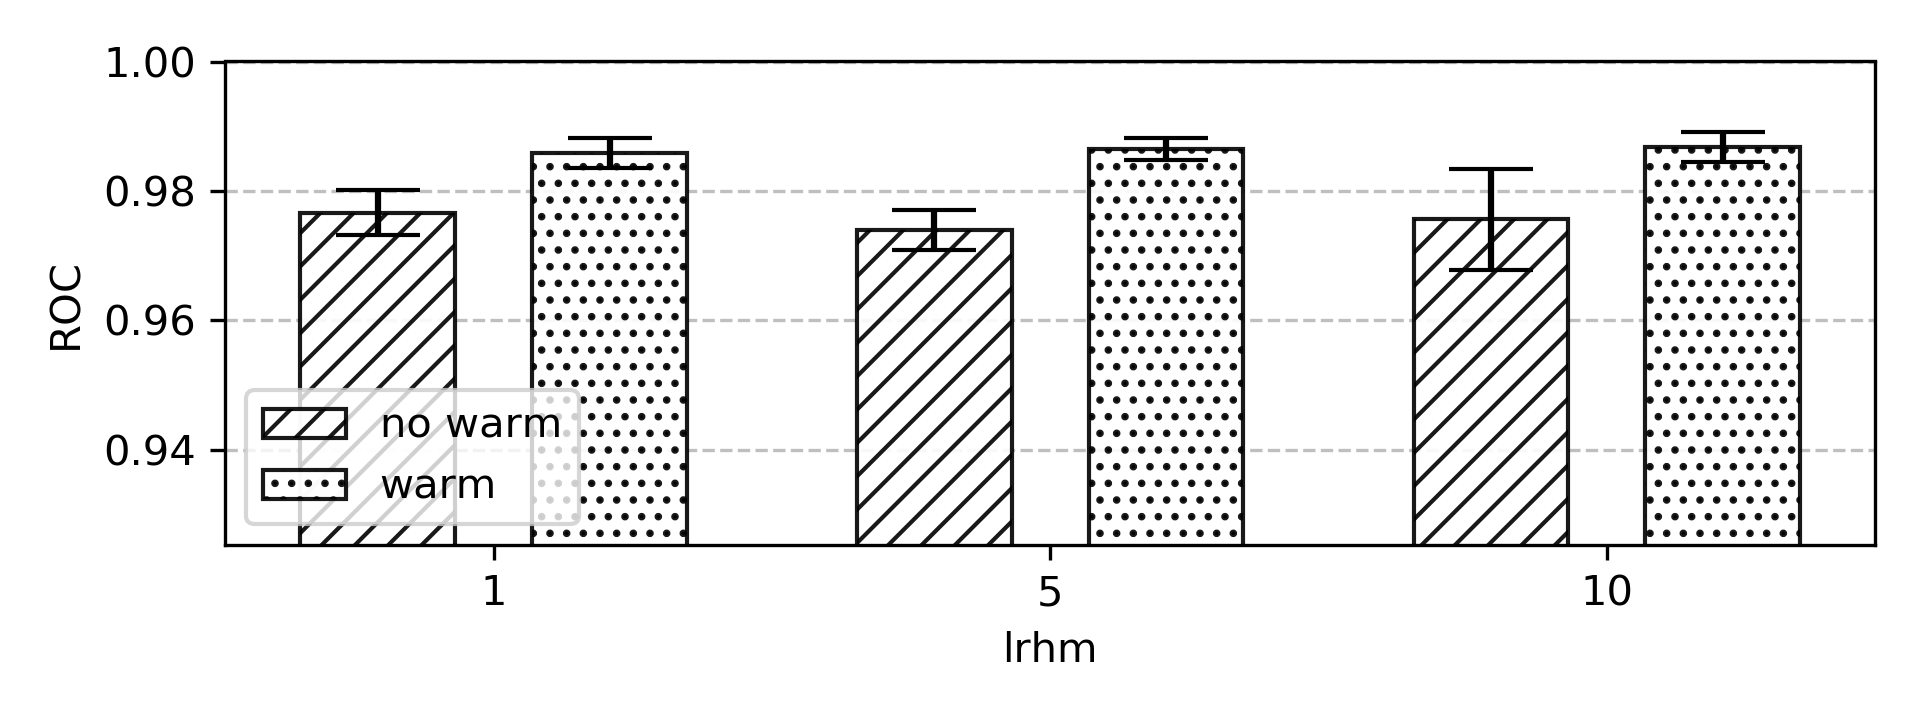
\includegraphics[scale=0.5]{images/all_plots/bar_lrhm_1e-4_densenet121_cells_no_aug.png}}
\subfigure[Glomeruli]{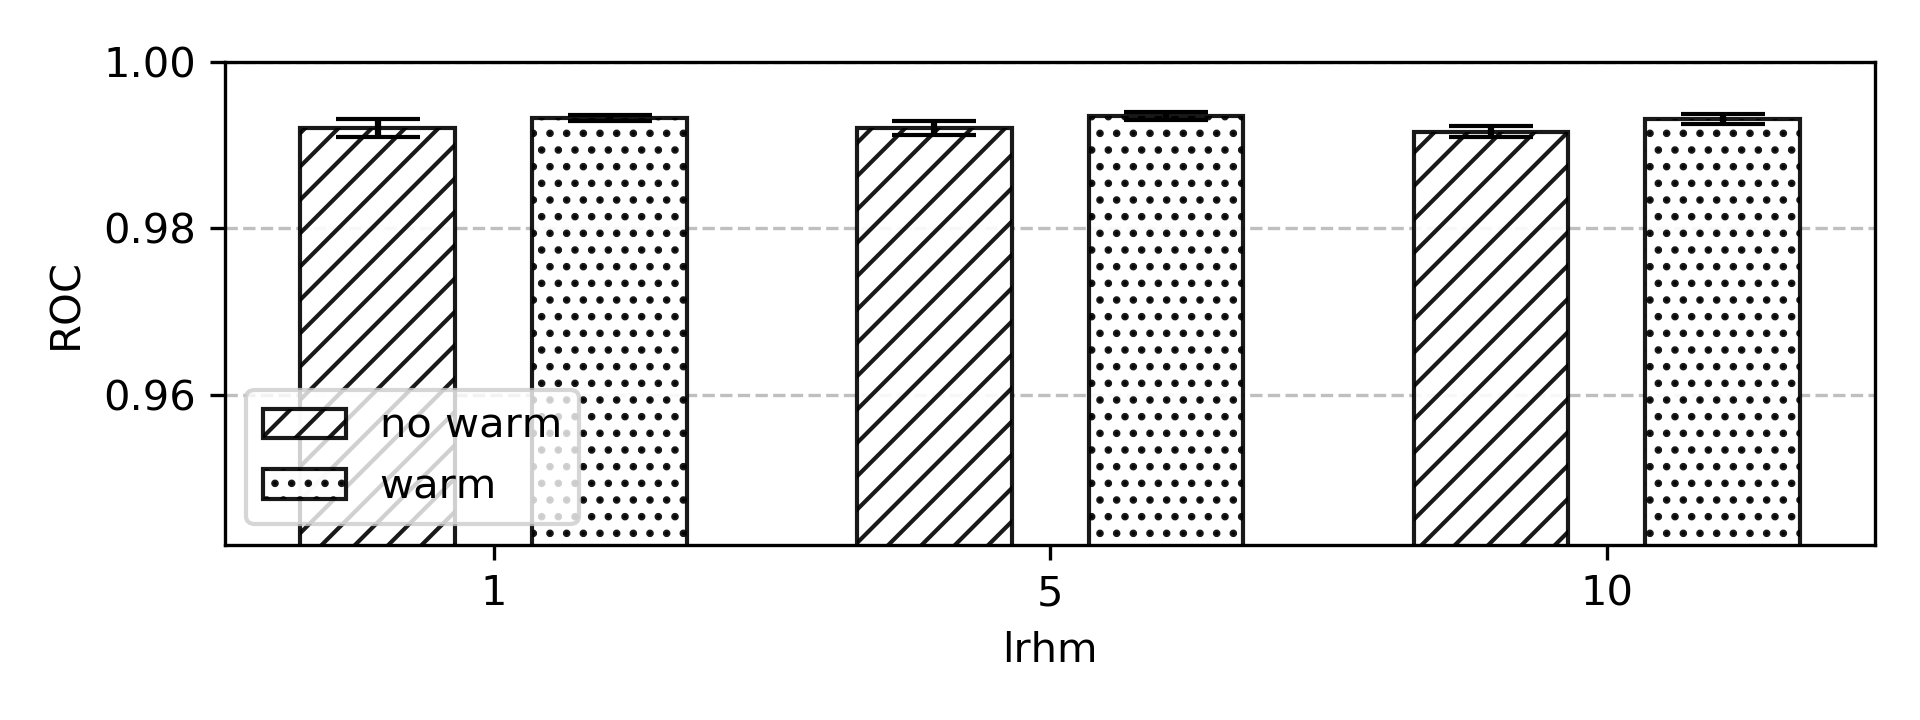
\includegraphics[scale=0.5]{images/all_plots/bar_lrhm_1e-4_densenet121_glomeruli_no_aug.png}}\\
\subfigure[ProliferativePattern]{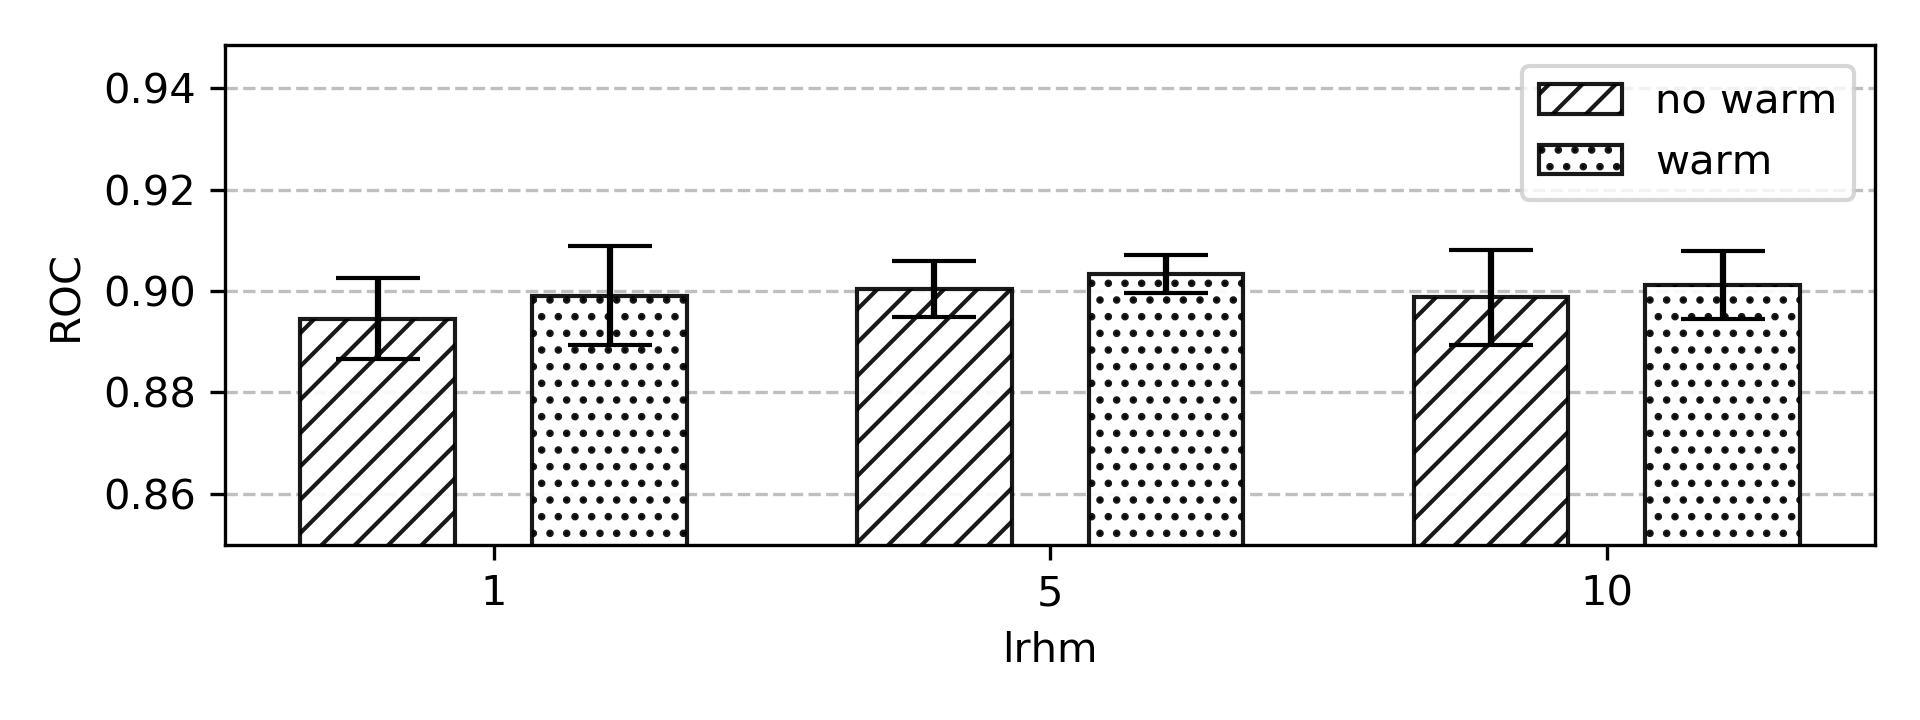
\includegraphics[scale=0.5]{images/all_plots/bar_lrhm_1e-4_densenet121_patterns_no_aug.png}}
\subfigure[HumanLba]{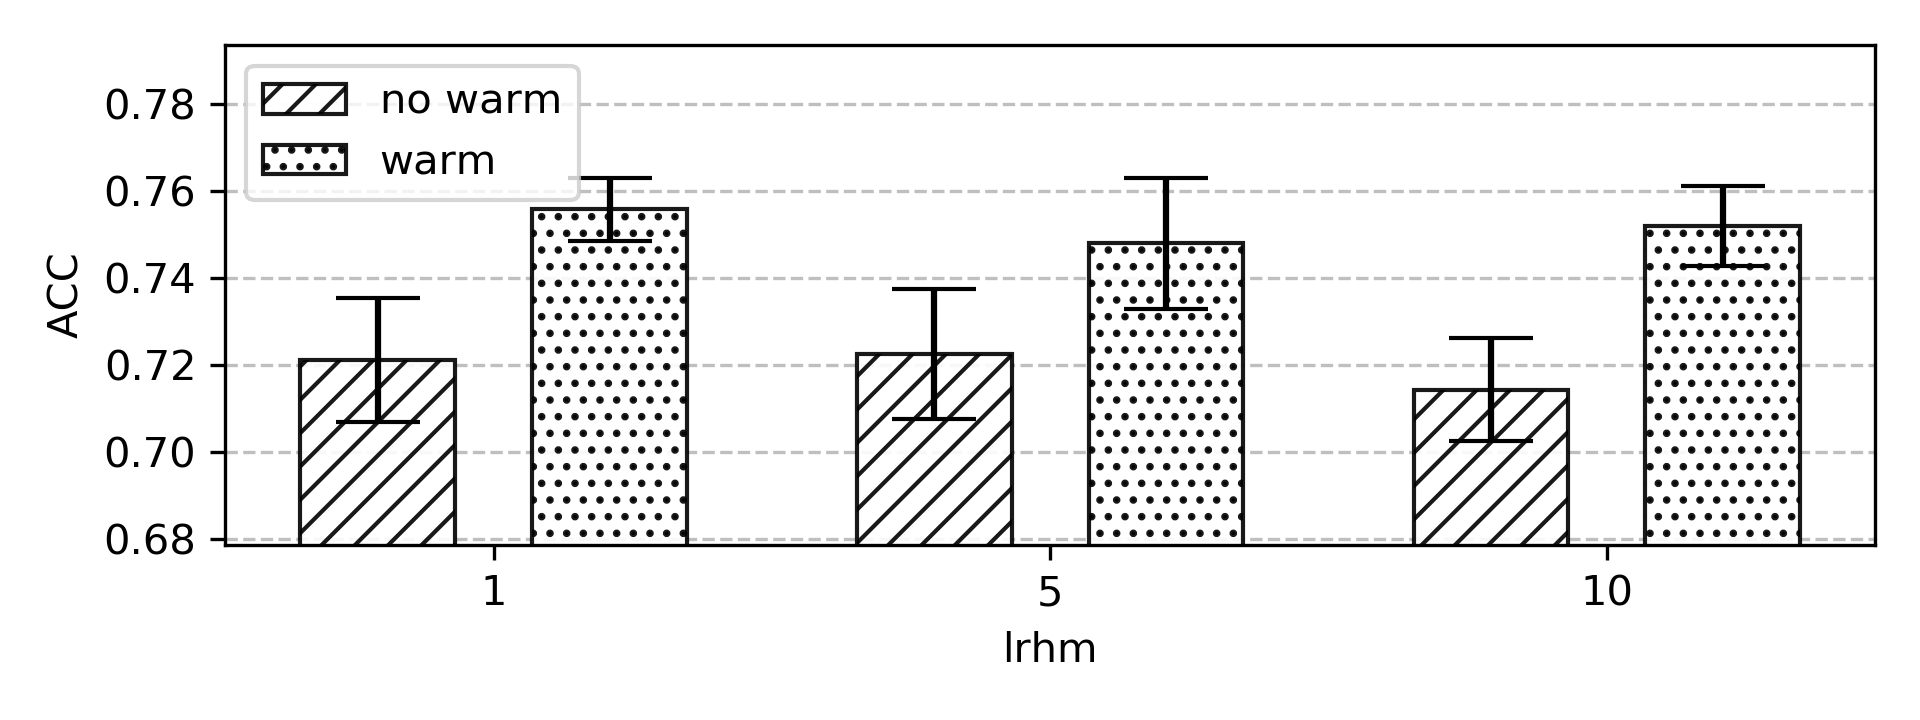
\includegraphics[scale=0.5]{images/all_plots/bar_lrhm_1e-4_densenet121_ulb_anapath_lba.png}}\\
\subfigure[BoneMarrow]{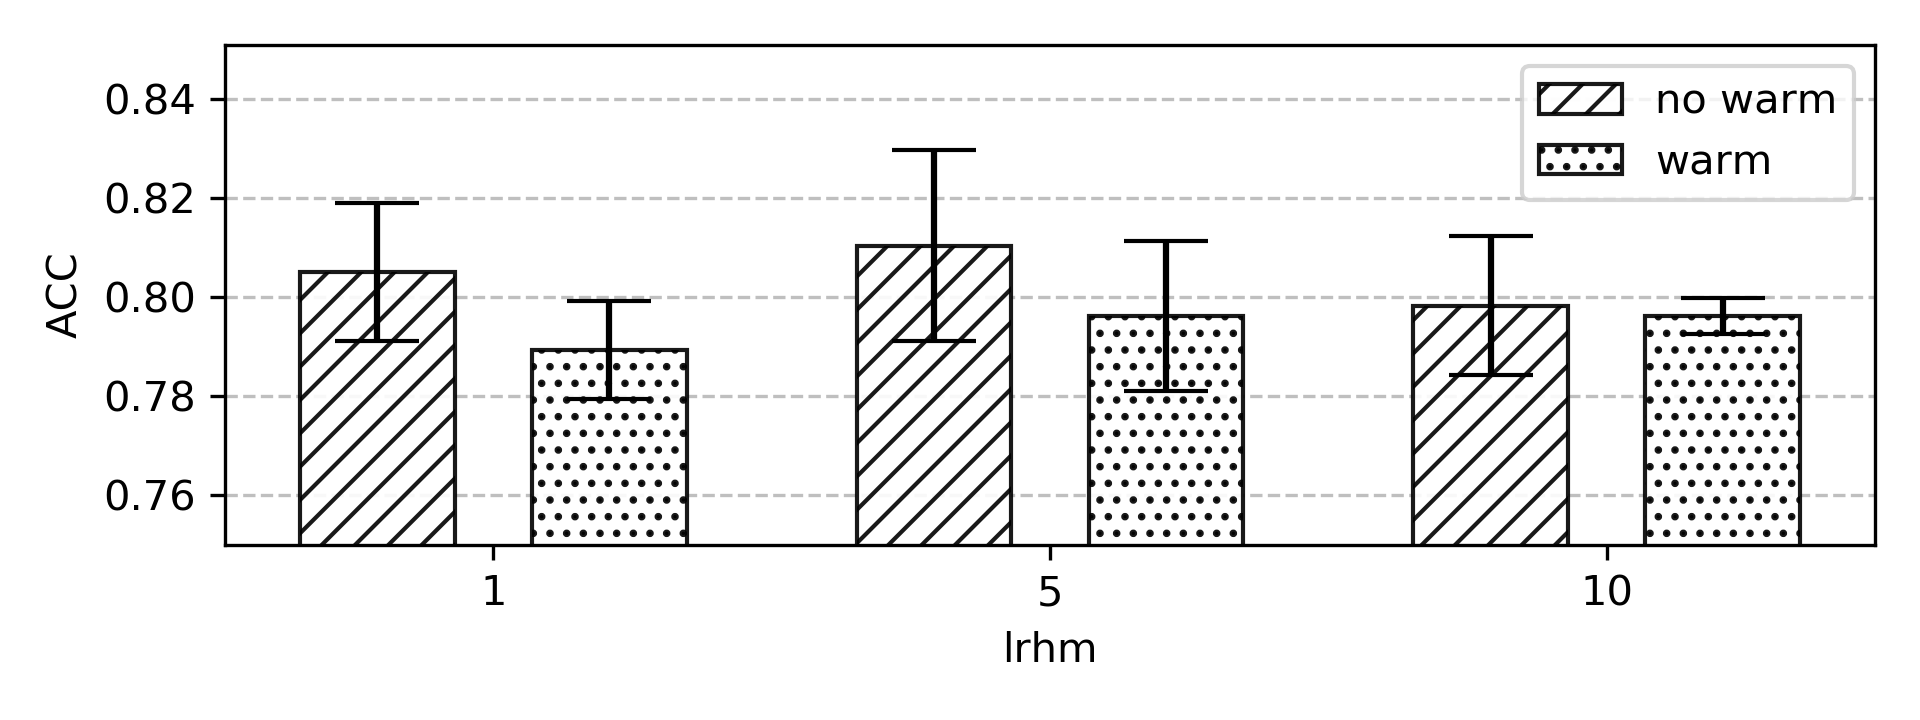
\includegraphics[scale=0.5]{images/all_plots/bar_lrhm_1e-4_densenet121_ulg_bonemarrow.png}}
\subfigure[Breast1]{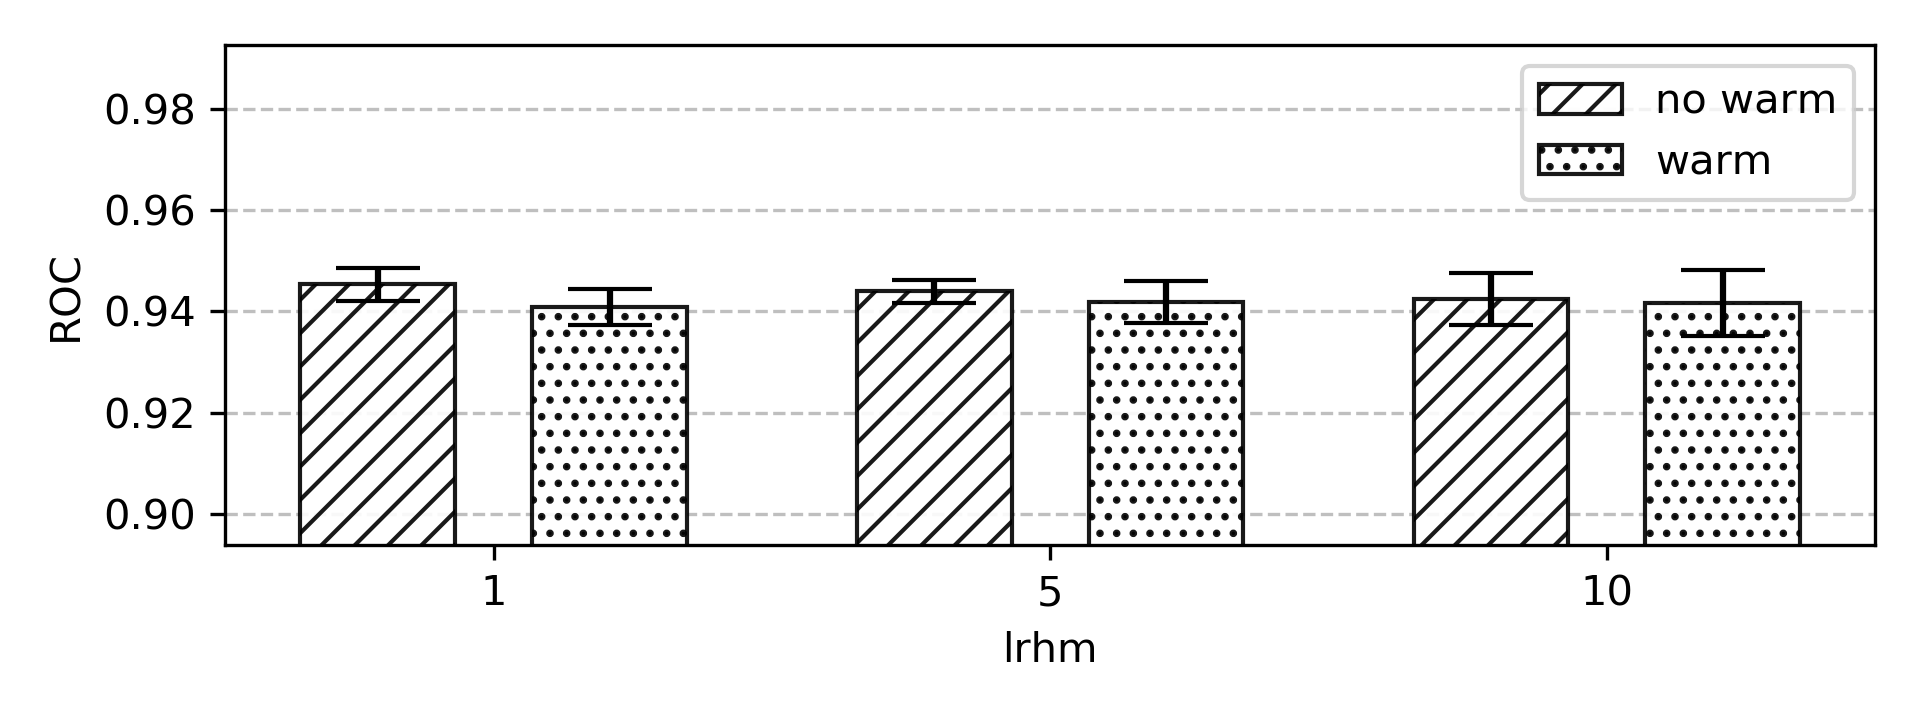
\includegraphics[scale=0.5]{images/all_plots/bar_lrhm_1e-4_densenet121_ulg_breast.png}}\\
\subfigure[Breast2]{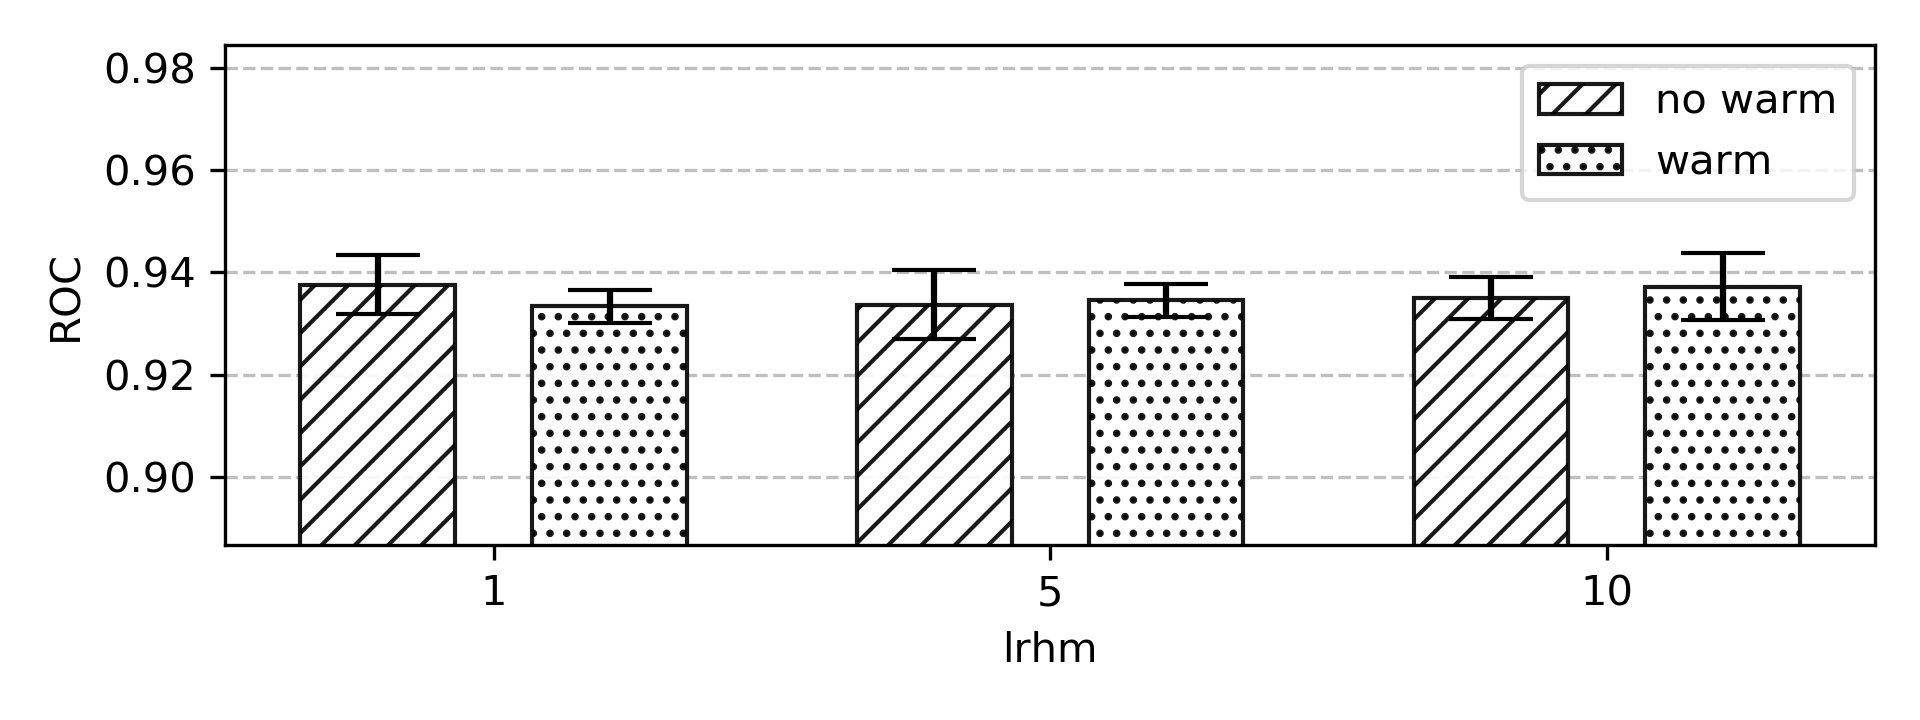
\includegraphics[scale=0.5]{images/all_plots/bar_lrhm_1e-4_densenet121_ulg_breast2.png}}
\subfigure[Necrose]{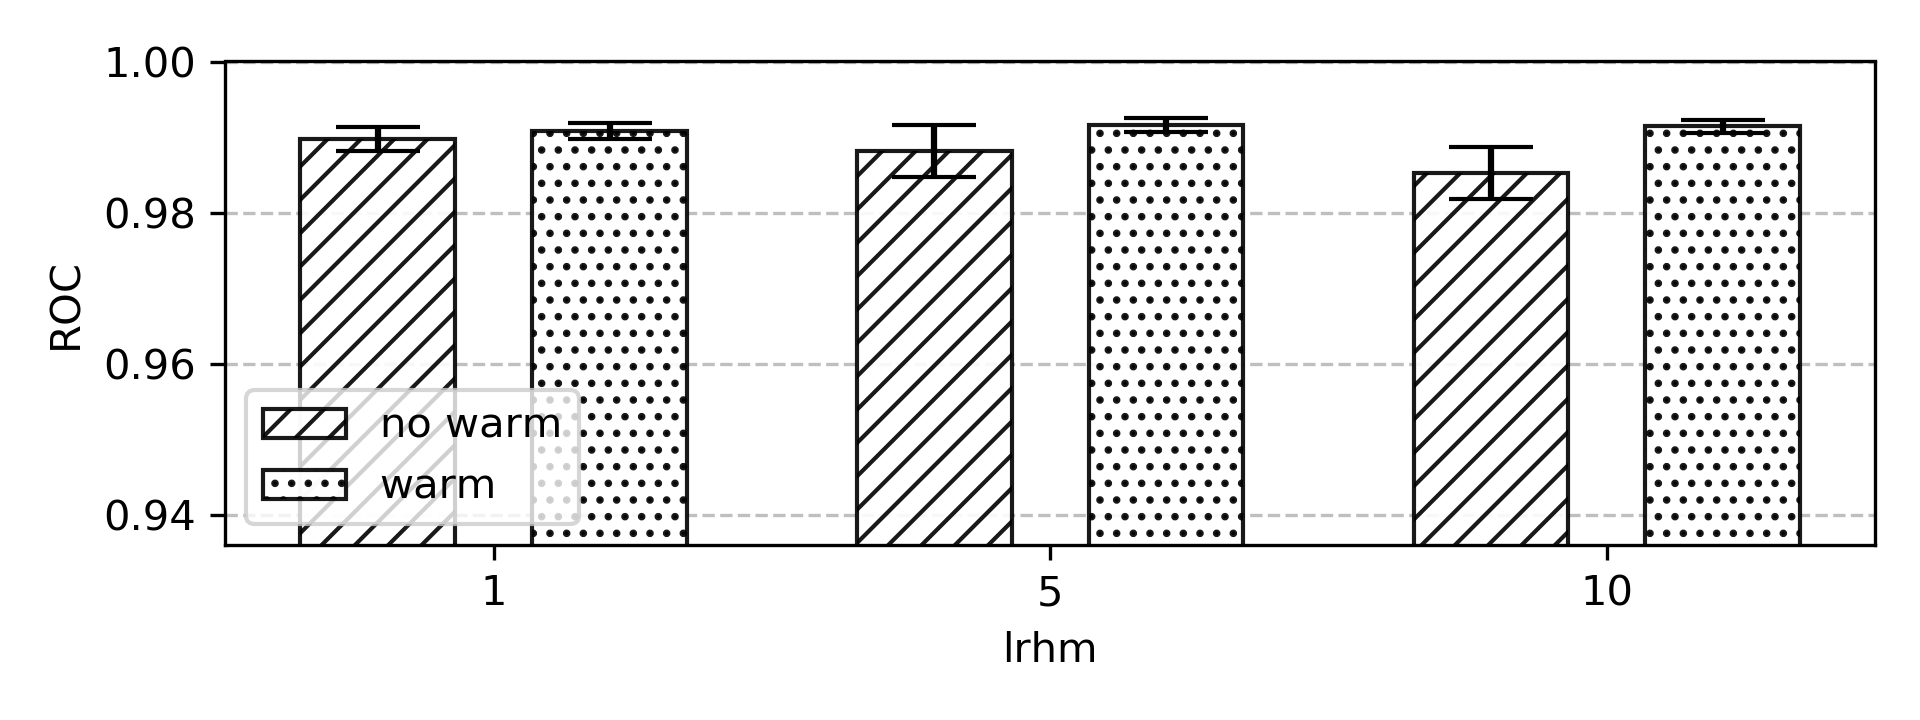
\includegraphics[scale=0.5]{images/all_plots/bar_lrhm_1e-4_densenet121_ulg_lbtd2_chimio_necrose.png}}\\
\subfigure[MouseLba]{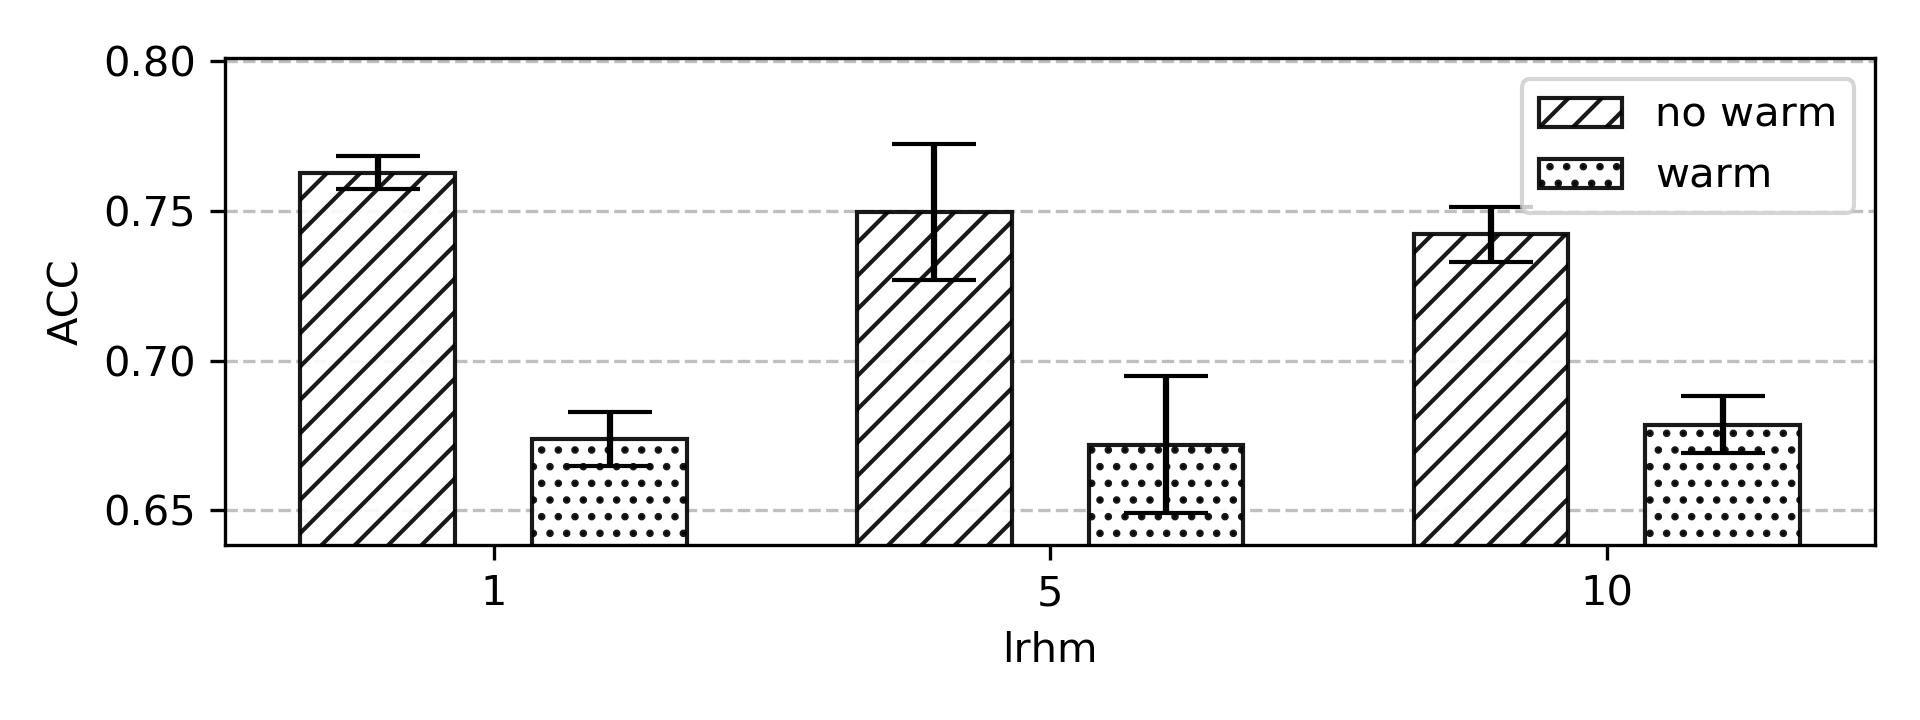
\includegraphics[scale=0.5]{images/all_plots/bar_lrhm_1e-4_densenet121_ulg_lbtd_lba.png}}
\subfigure[Lung]{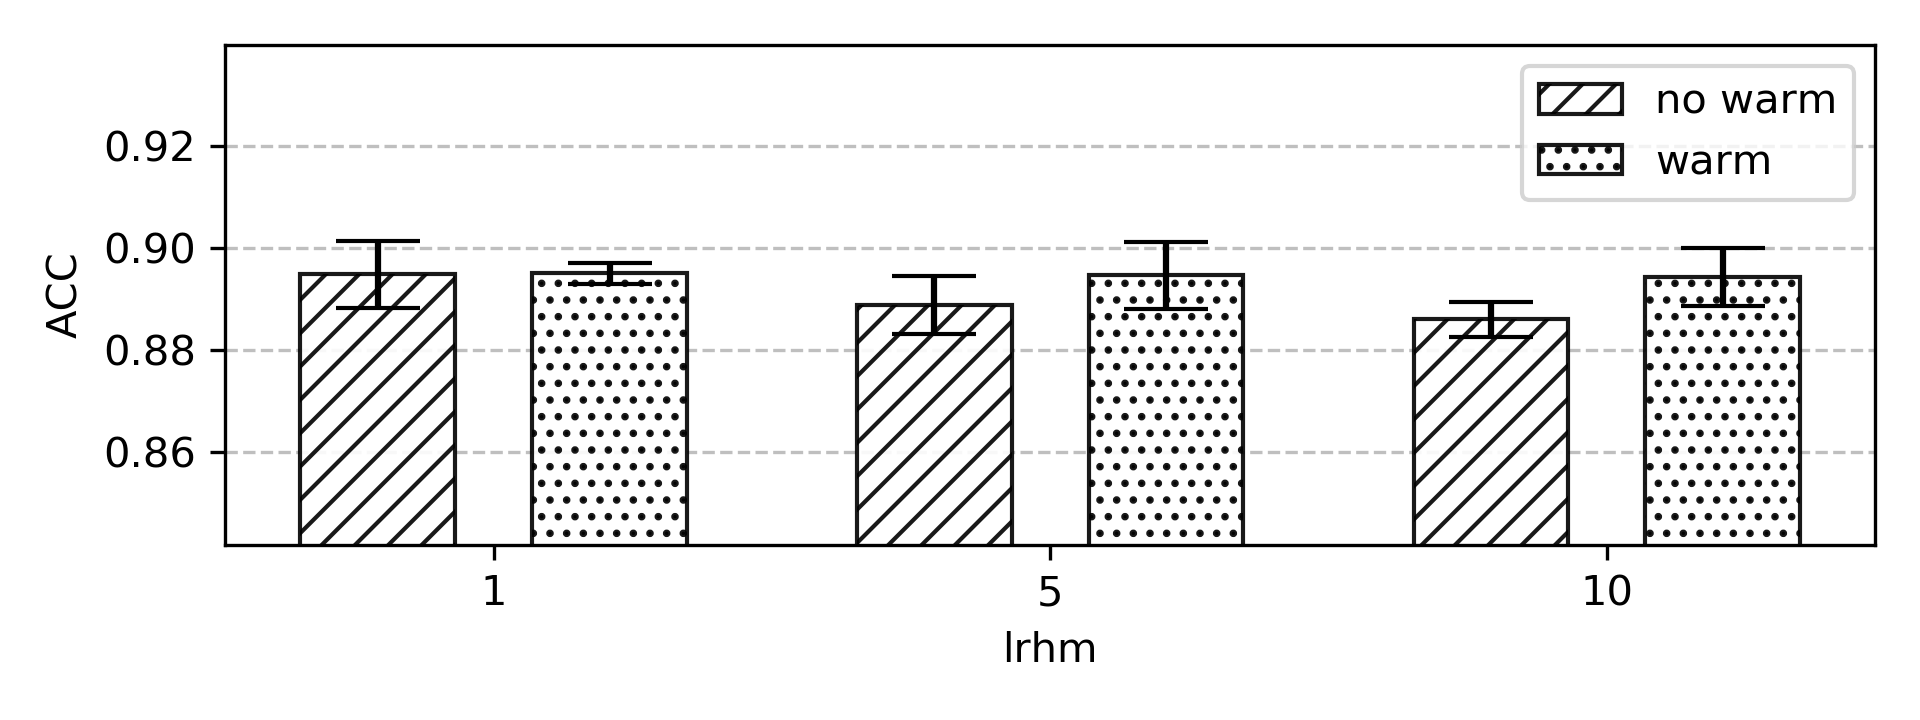
\includegraphics[scale=0.5]{images/all_plots/bar_lrhm_1e-4_densenet121_ulg_lbtd_tissus.png}}
    \caption{Transfer performance for combinations of the hyperparameters $\gamma_\tau$ (learning rate heads multiplier) and $w$ (warm up) with learning rate $\gamma = 10^{-4}$ on DenseNet121.}
    \label{app:mtask:fig:app:bar_lrhm_densenet}
\end{figure*}

\begin{figure*}[h]
    \centering
\subfigure[CellInclusion]{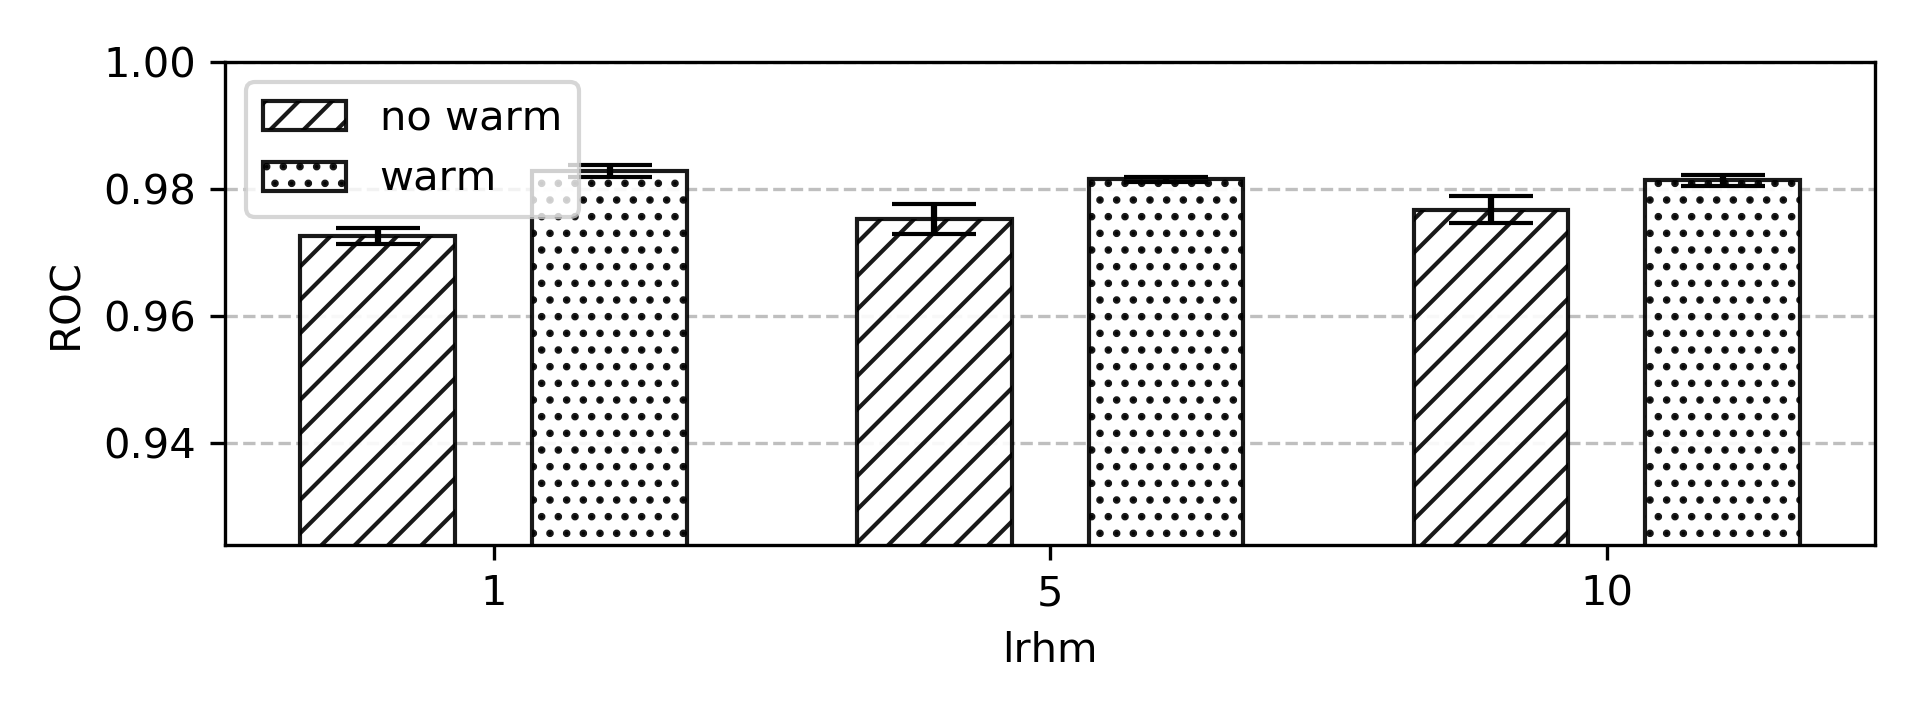
\includegraphics[scale=0.5]{images/all_plots/bar_lrhm_1e-4_resnet50_cells_no_aug.png}}
\subfigure[Glomeruli]{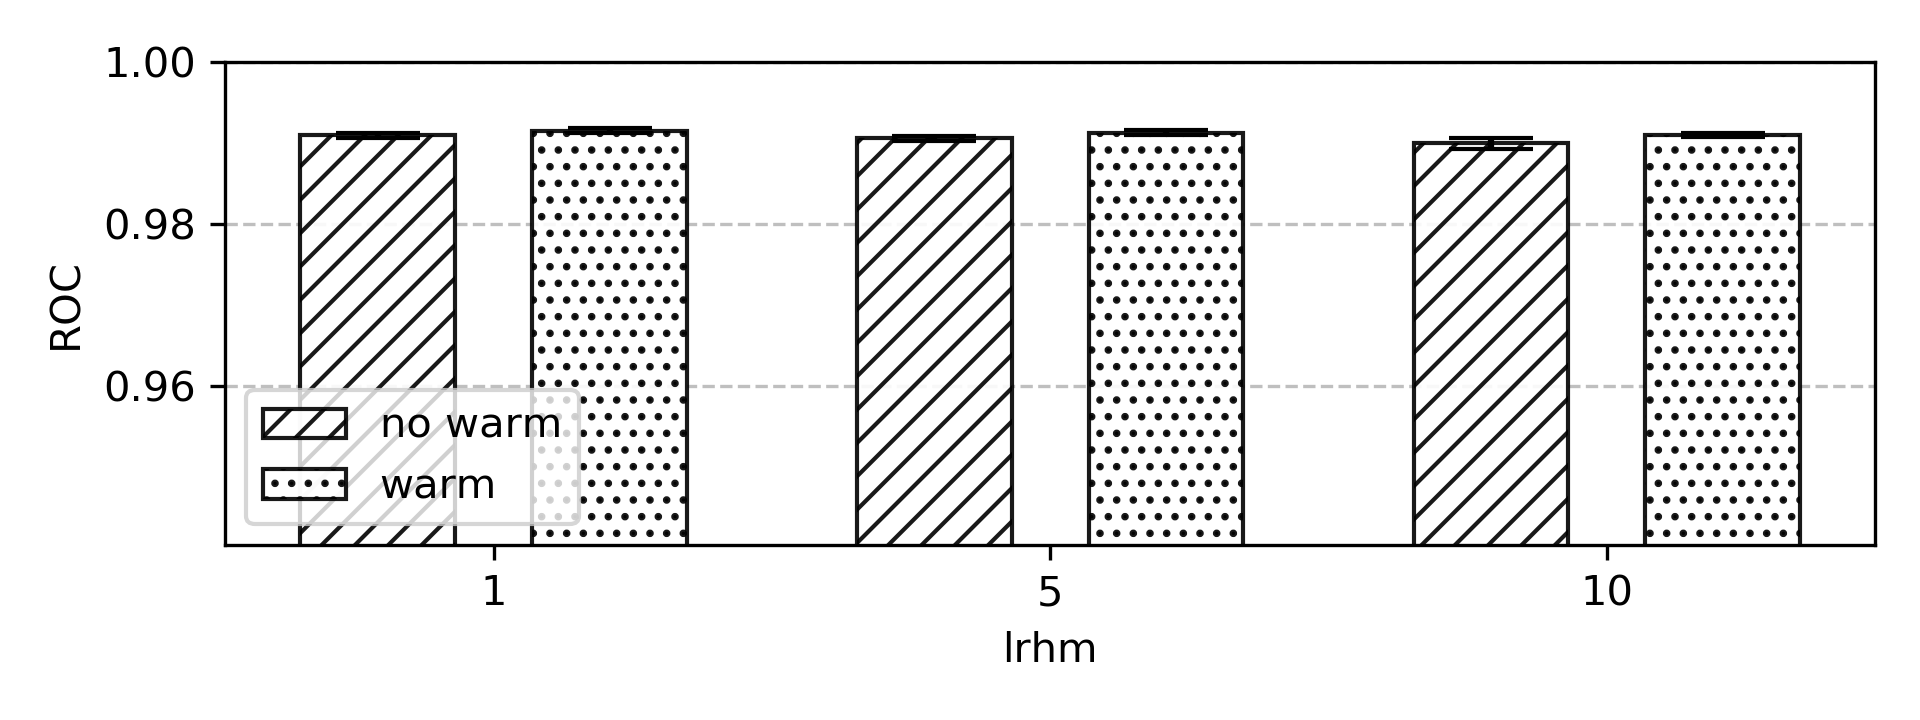
\includegraphics[scale=0.5]{images/all_plots/bar_lrhm_1e-4_resnet50_glomeruli_no_aug.png}}\\
\subfigure[ProliferativePattern]{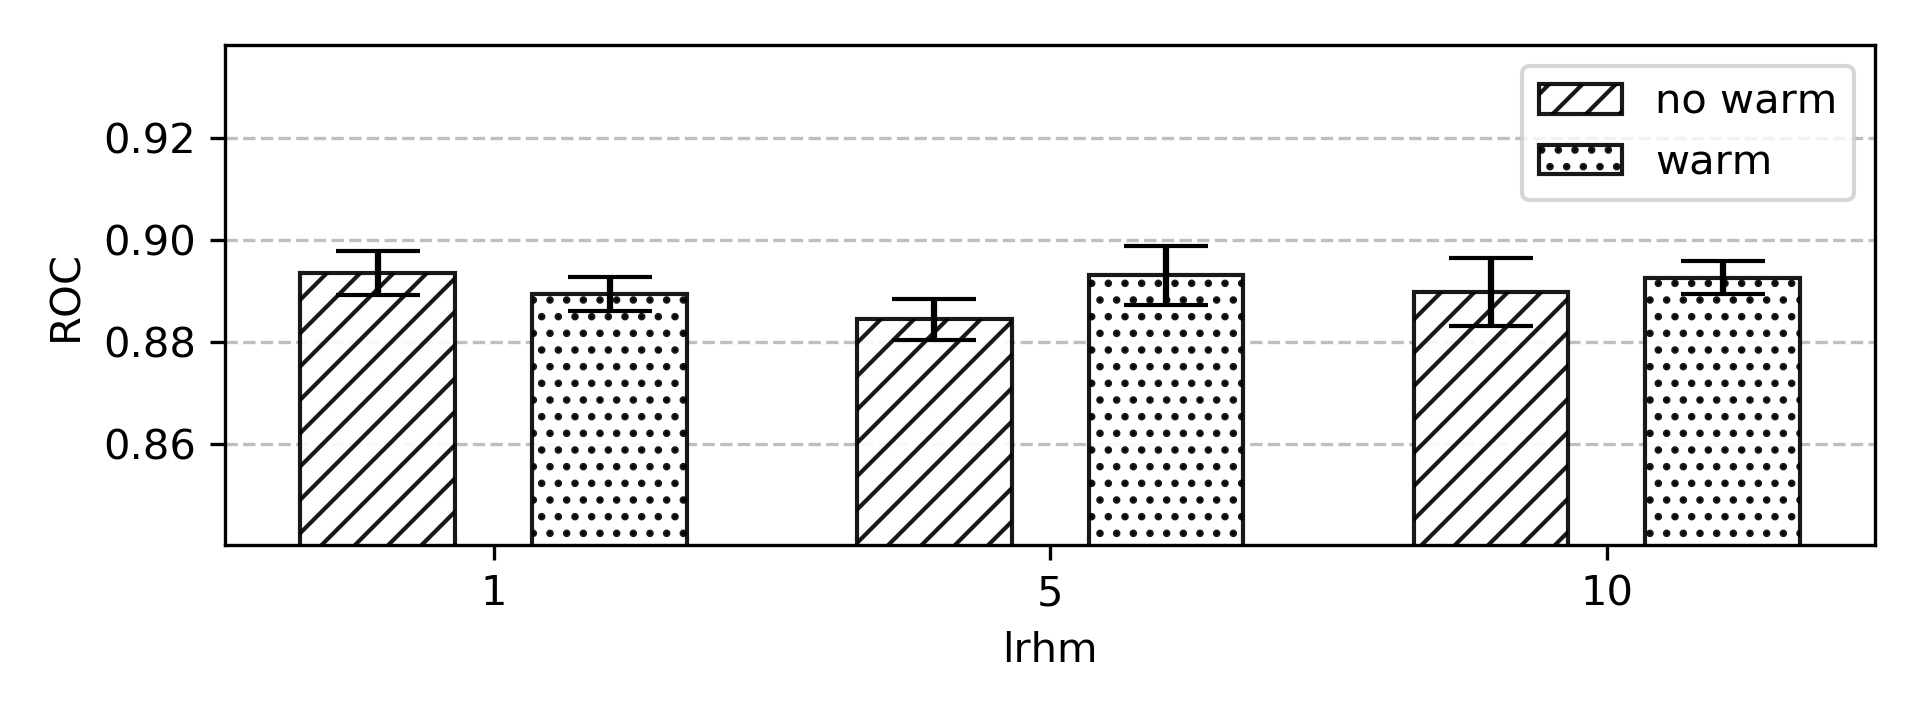
\includegraphics[scale=0.5]{images/all_plots/bar_lrhm_1e-4_resnet50_patterns_no_aug.png}}
\subfigure[HumanLba]{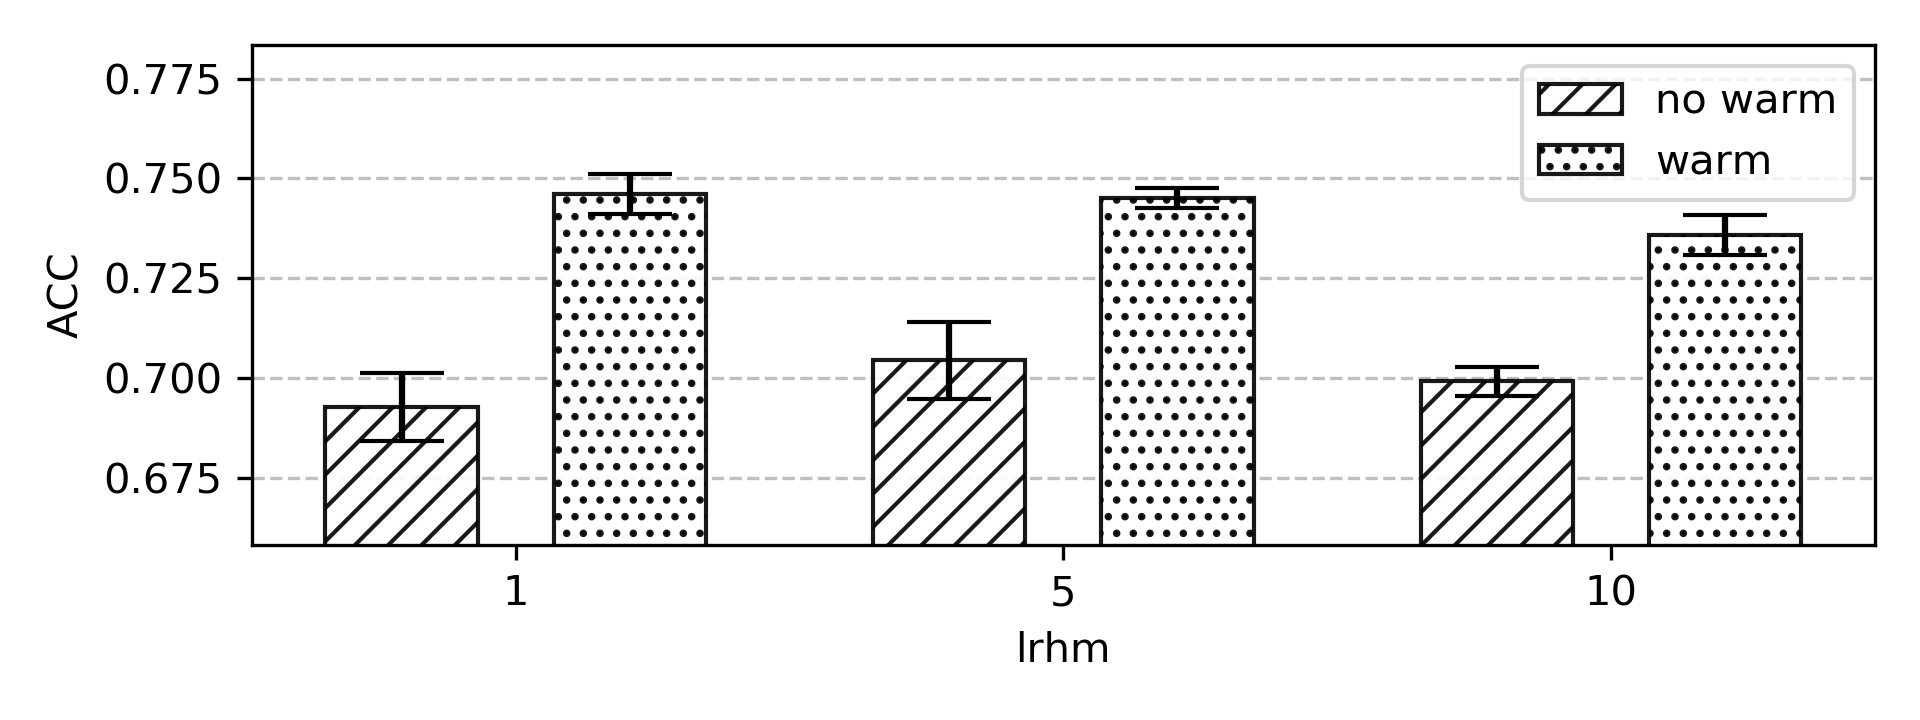
\includegraphics[scale=0.5]{images/all_plots/bar_lrhm_1e-4_resnet50_ulb_anapath_lba.png}}\\
\subfigure[BoneMarrow]{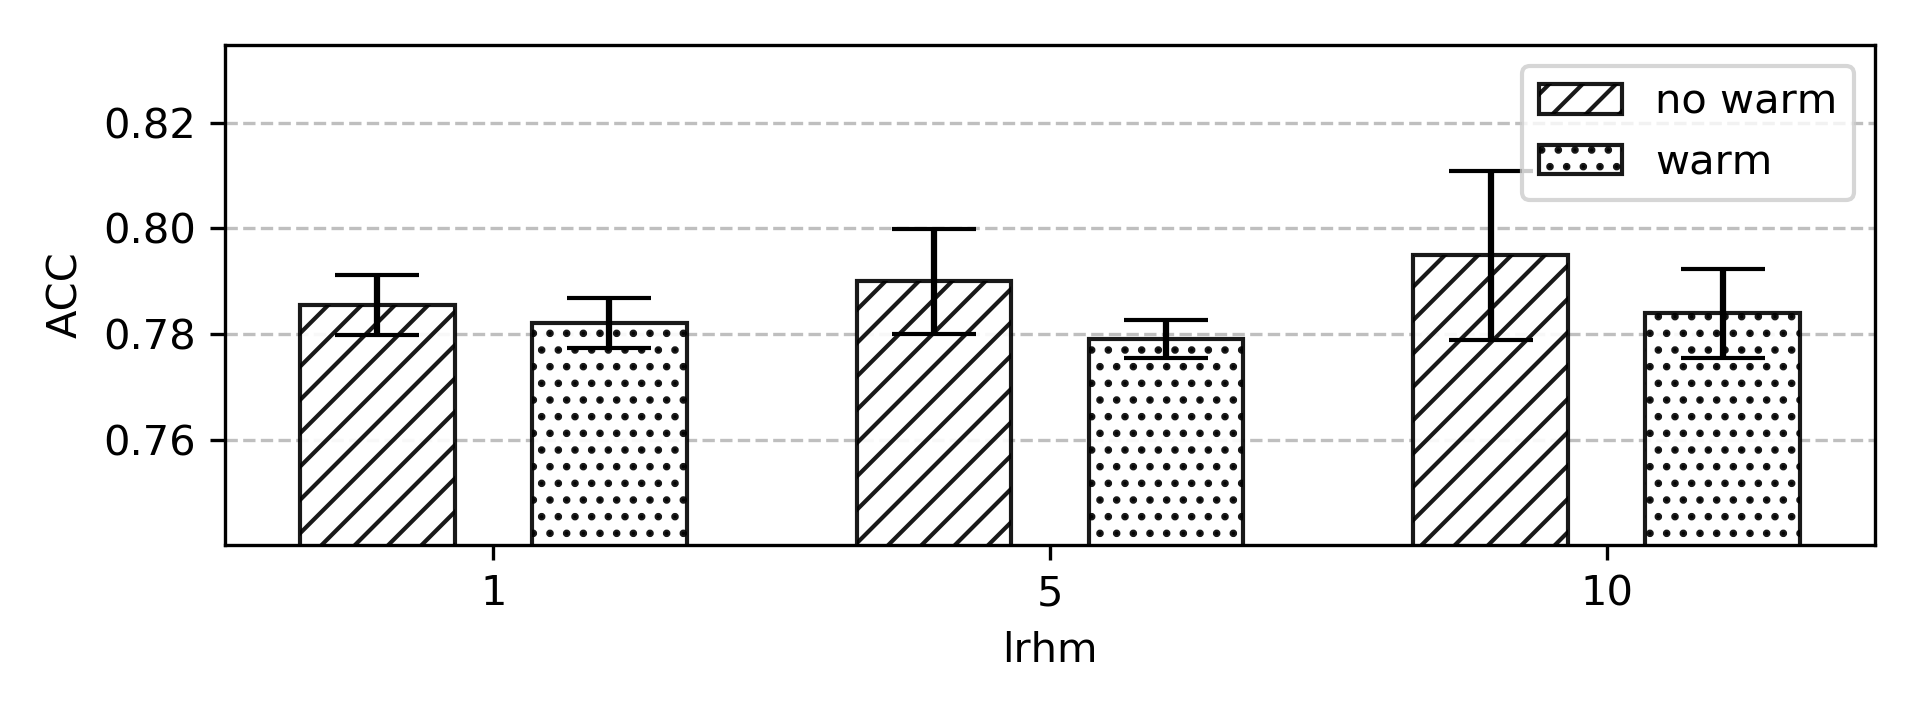
\includegraphics[scale=0.5]{images/all_plots/bar_lrhm_1e-4_resnet50_ulg_bonemarrow.png}}
\subfigure[Breast1]{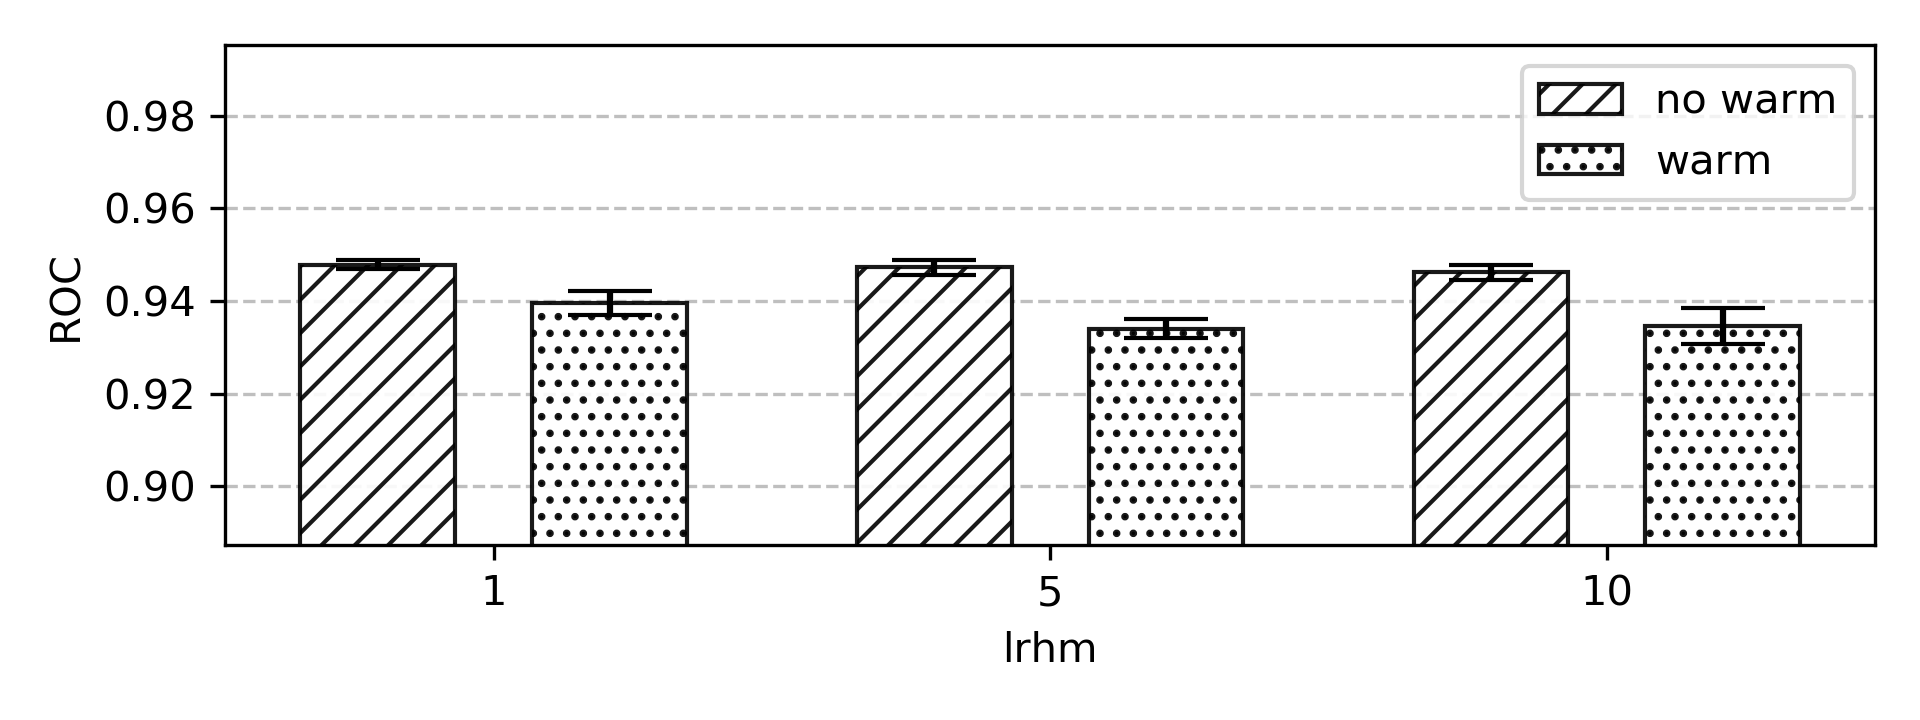
\includegraphics[scale=0.5]{images/all_plots/bar_lrhm_1e-4_resnet50_ulg_breast.png}}\\
\subfigure[Breast2]{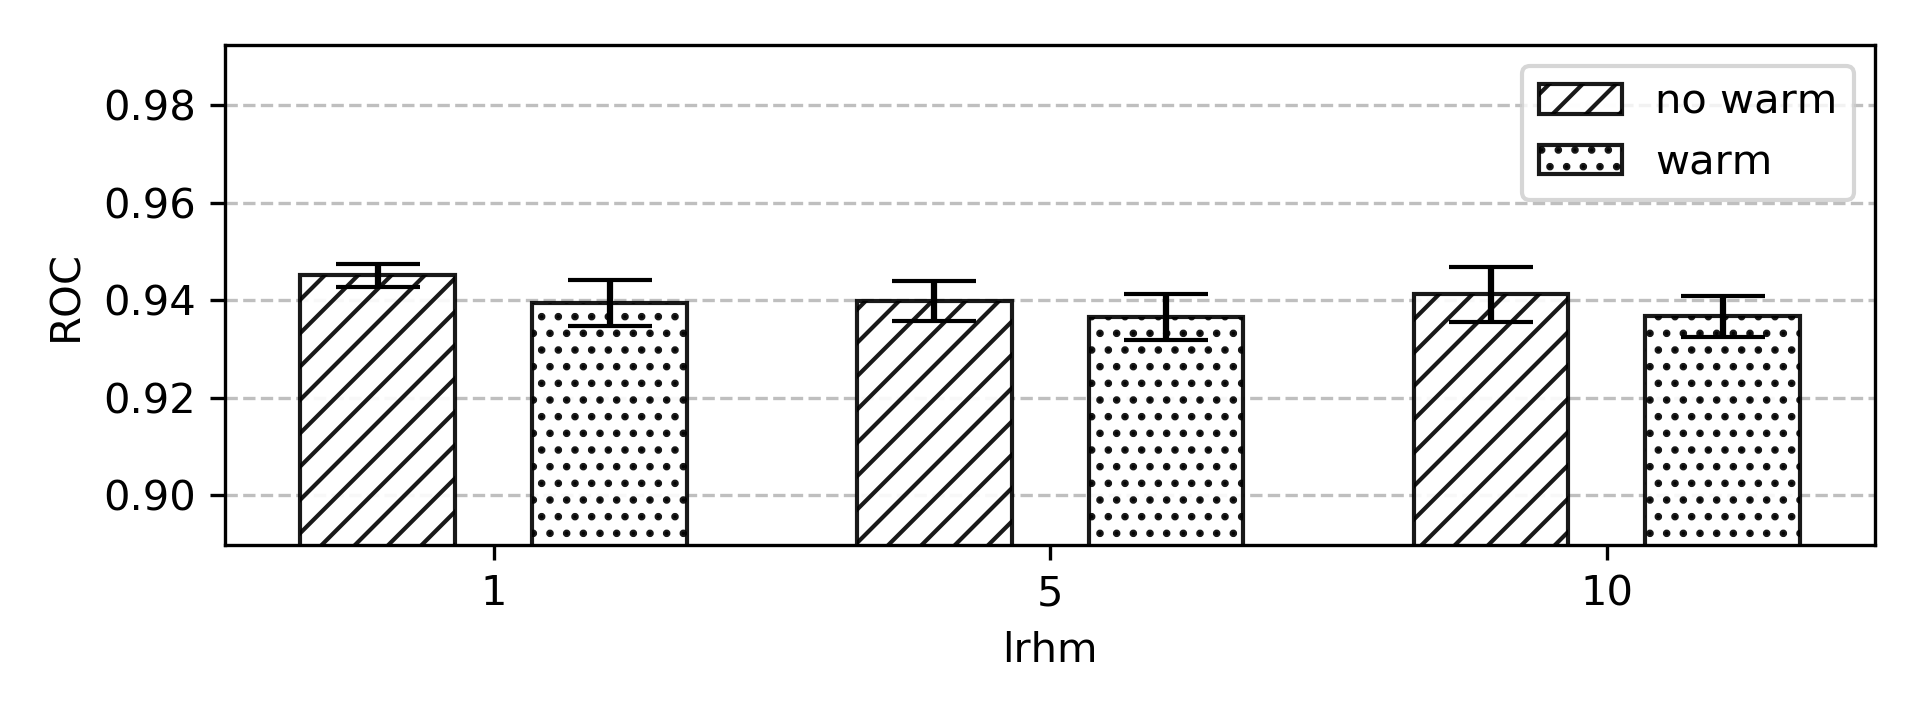
\includegraphics[scale=0.5]{images/all_plots/bar_lrhm_1e-4_resnet50_ulg_breast2.png}}
\subfigure[Necrose]{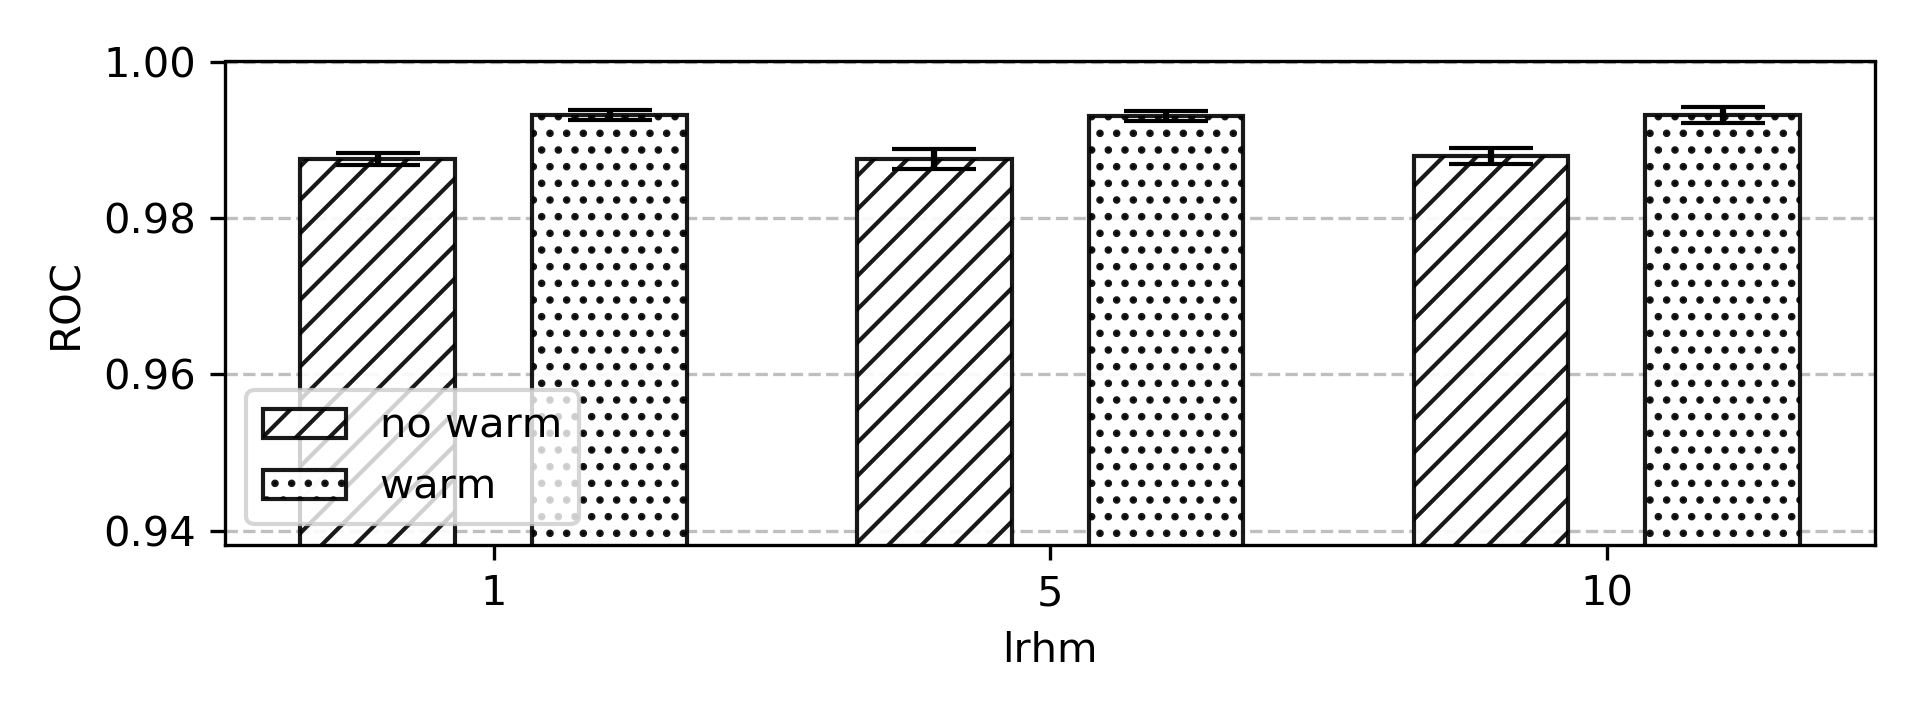
\includegraphics[scale=0.5]{images/all_plots/bar_lrhm_1e-4_resnet50_ulg_lbtd2_chimio_necrose.png}}\\
\subfigure[MouseLba]{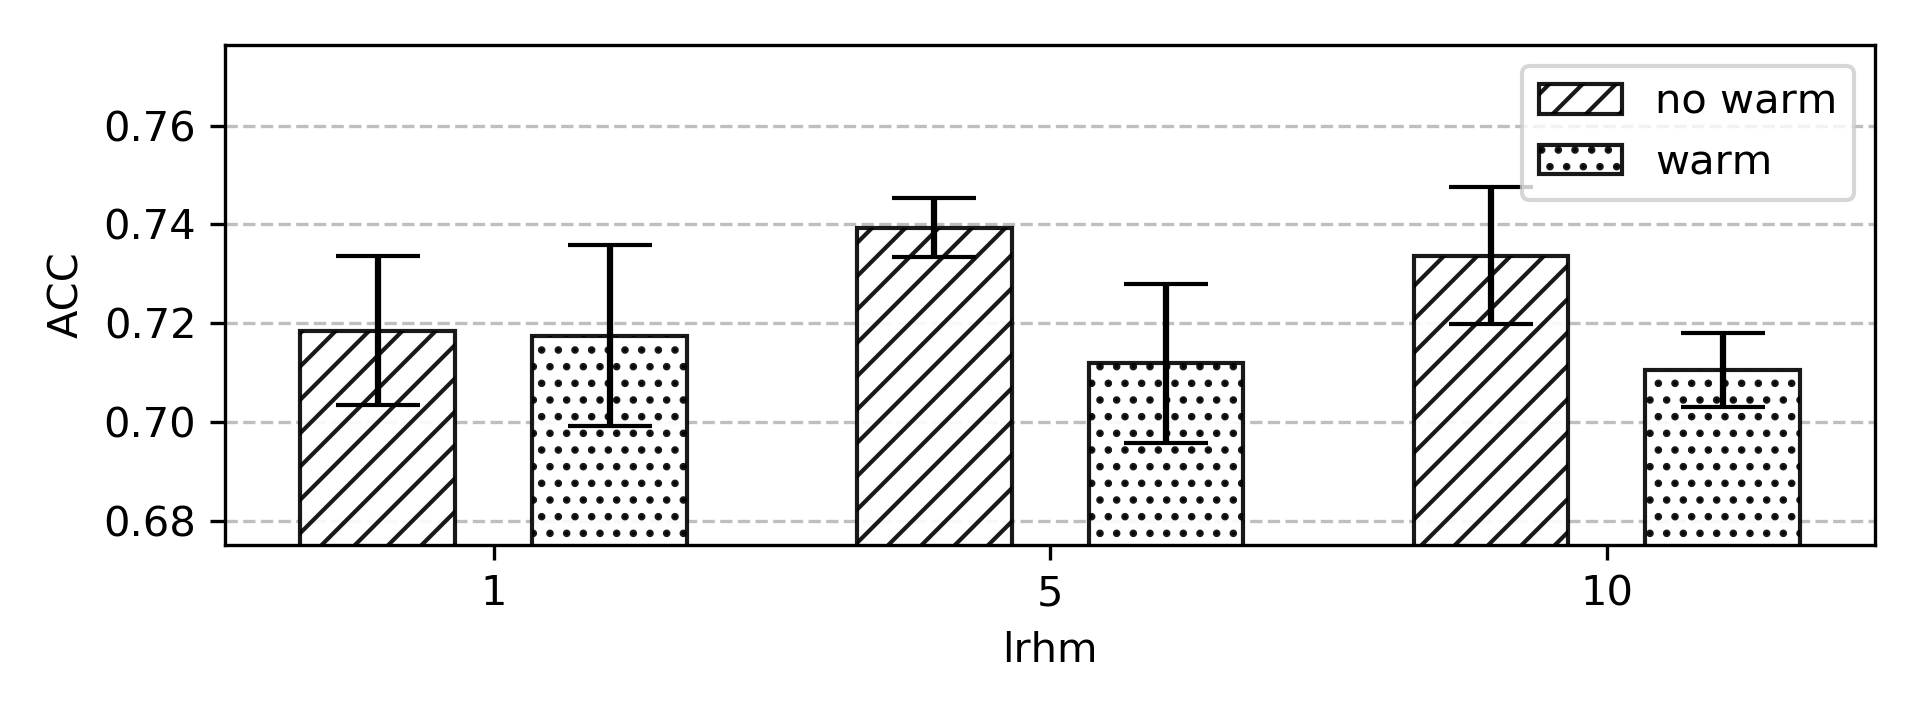
\includegraphics[scale=0.5]{images/all_plots/bar_lrhm_1e-4_resnet50_ulg_lbtd_lba.png}}
\subfigure[Lung]{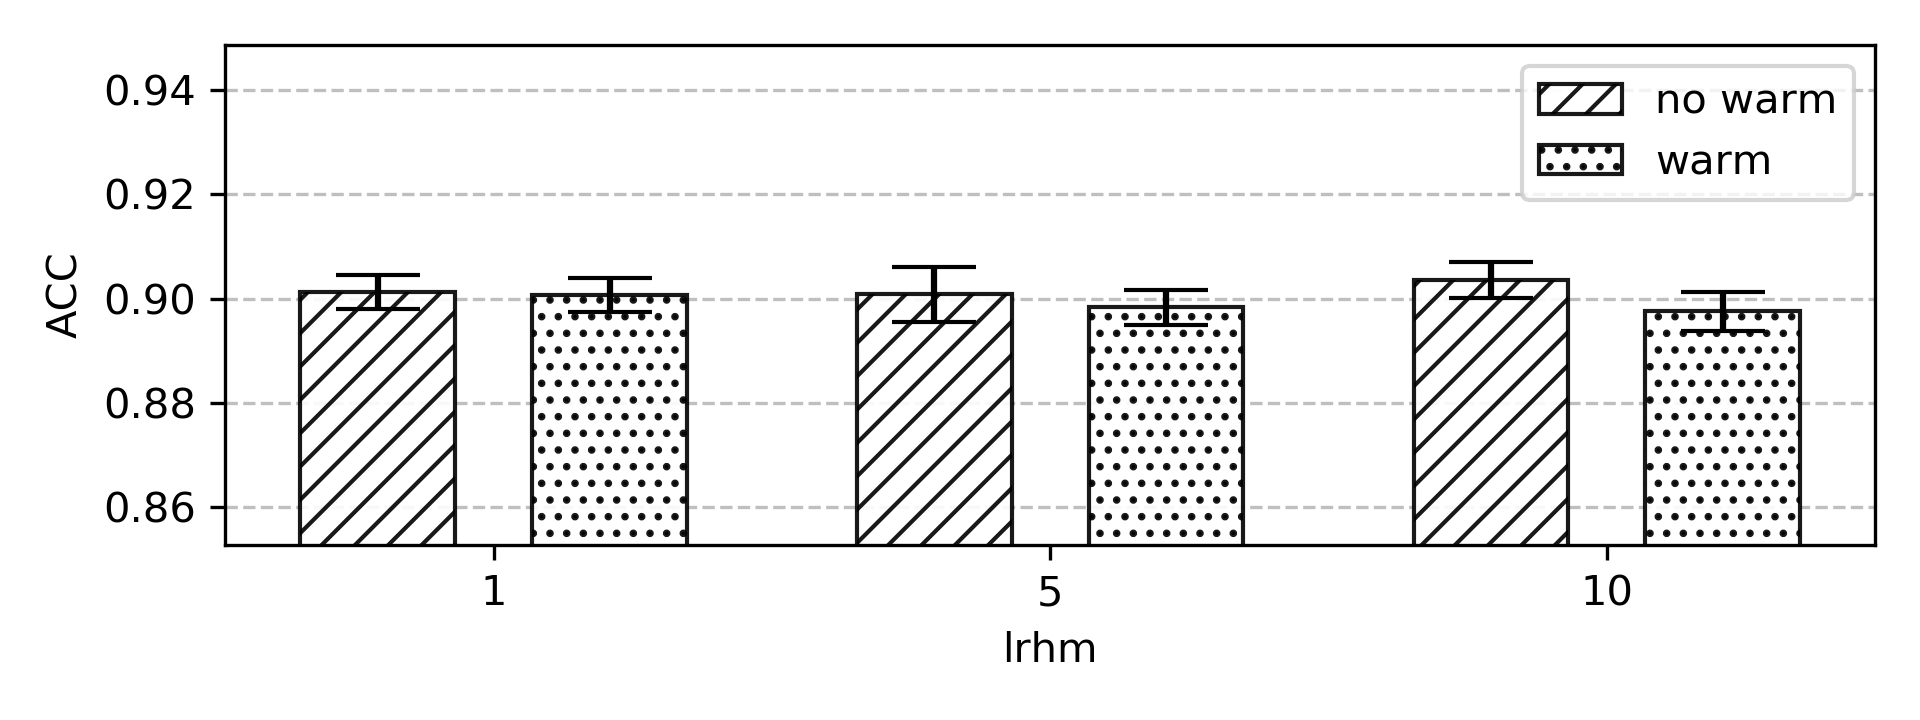
\includegraphics[scale=0.5]{images/all_plots/bar_lrhm_1e-4_resnet50_ulg_lbtd_tissus.png}}
    \caption{Transfer performance for combinations of the hyperparameters $\gamma_\tau$ (learning rate heads multiplier) and $w$ (warm up) with learning rate $\gamma = 10^{-4}$ on ResNet50.}
    \label{app:mtask:fig:app:bar_lrhm_resnet}
\end{figure*}

\begin{figure*}[h]
    \centering
\subfigure[CellInclusion]{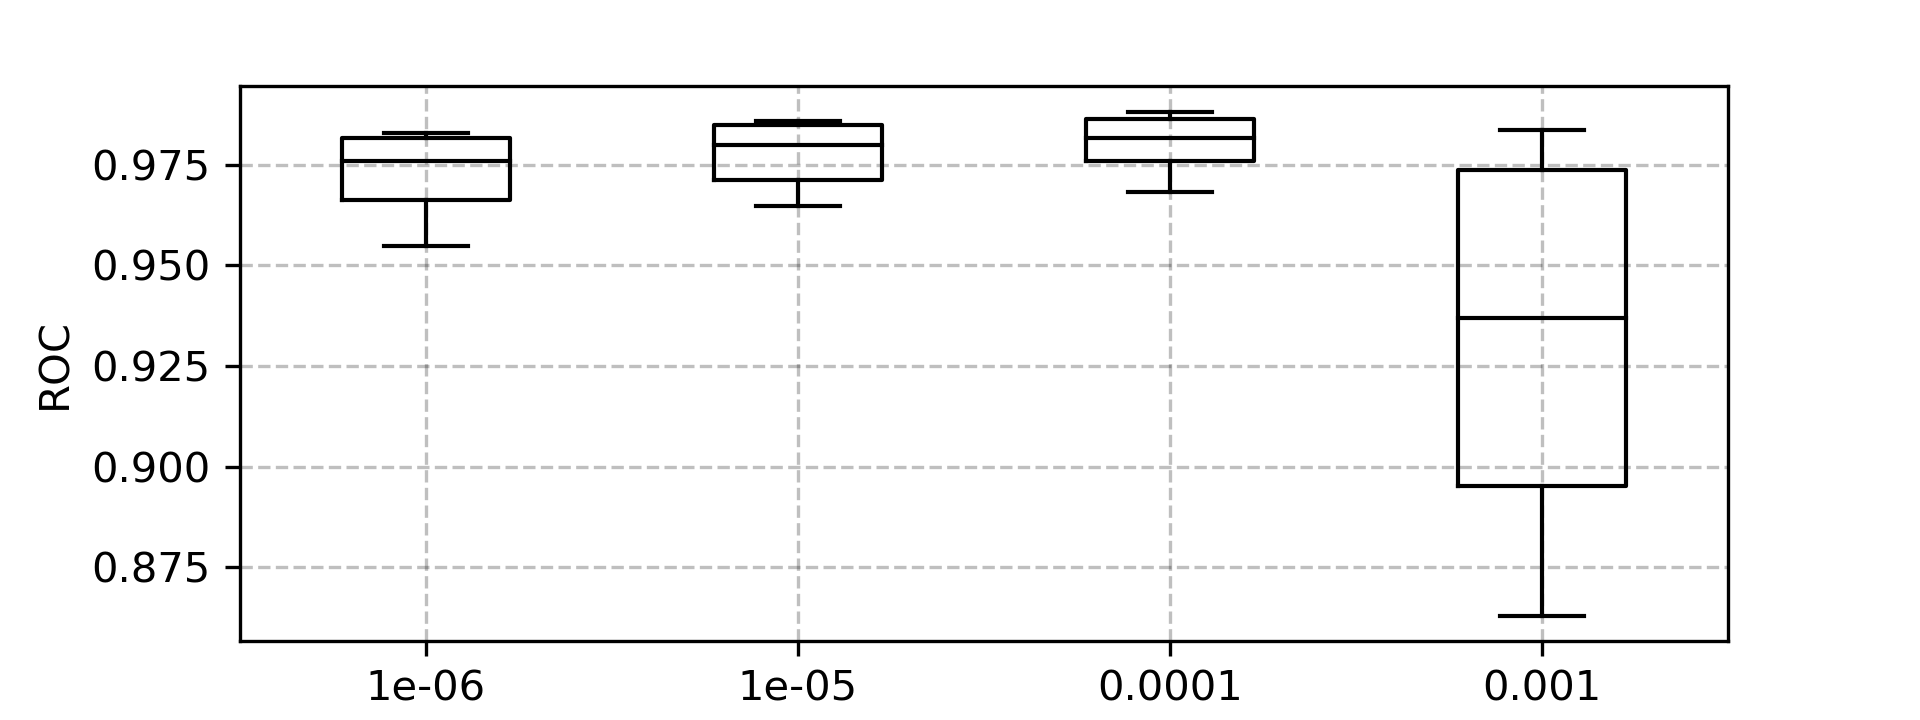
\includegraphics[scale=0.5]{images/all_plots/densenet121_cells_no_aug_learning_rate.png}}
\subfigure[Glomeruli]{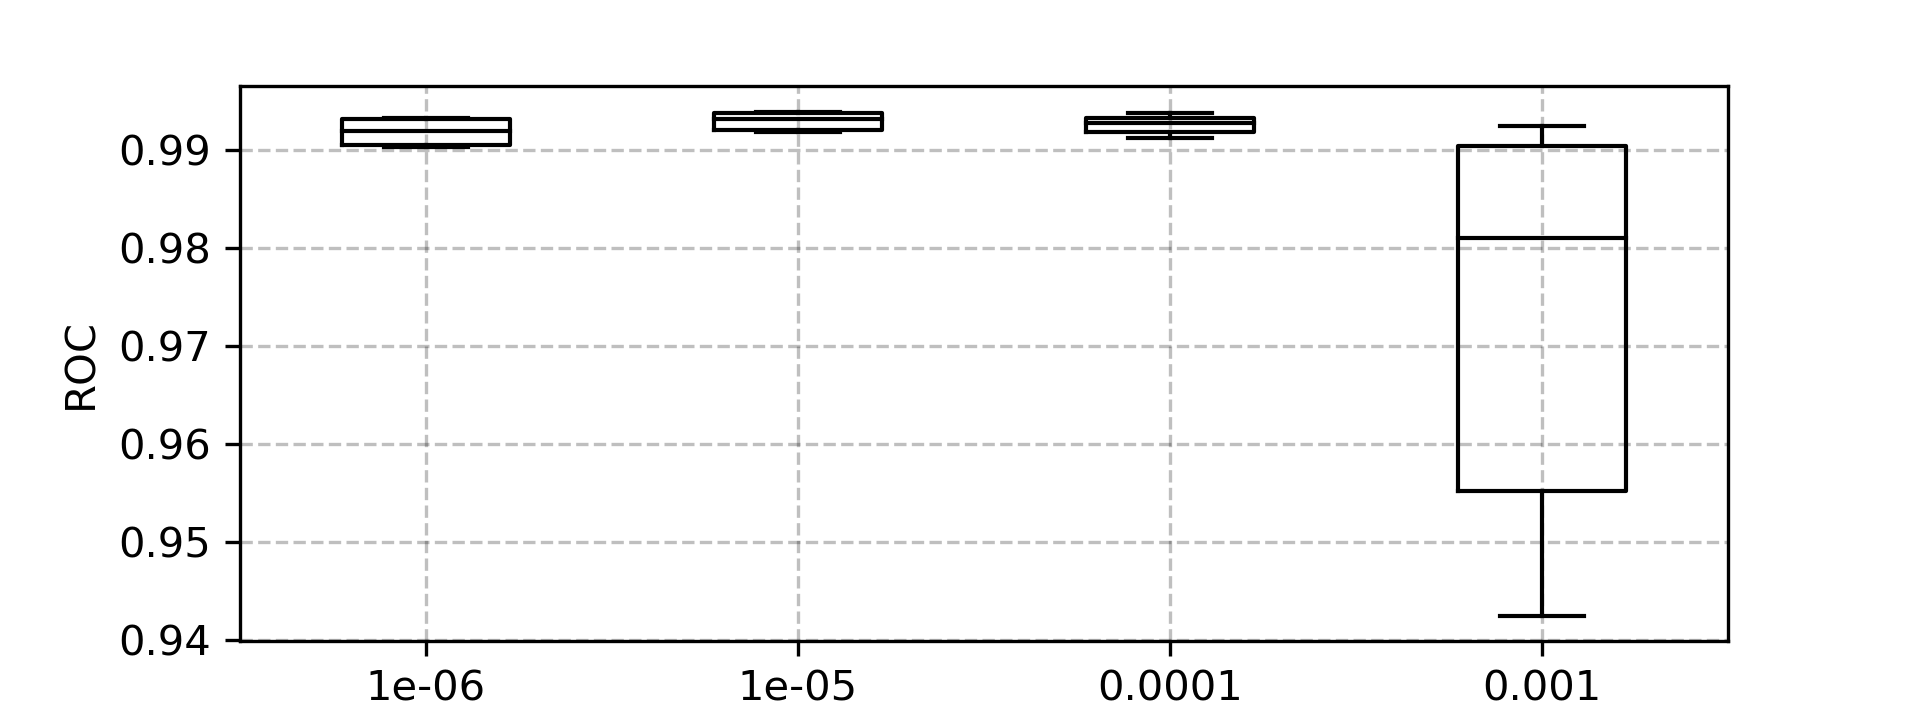
\includegraphics[scale=0.5]{images/all_plots/densenet121_glomeruli_no_aug_learning_rate.png}}\\
\subfigure[ProliferativePattern]{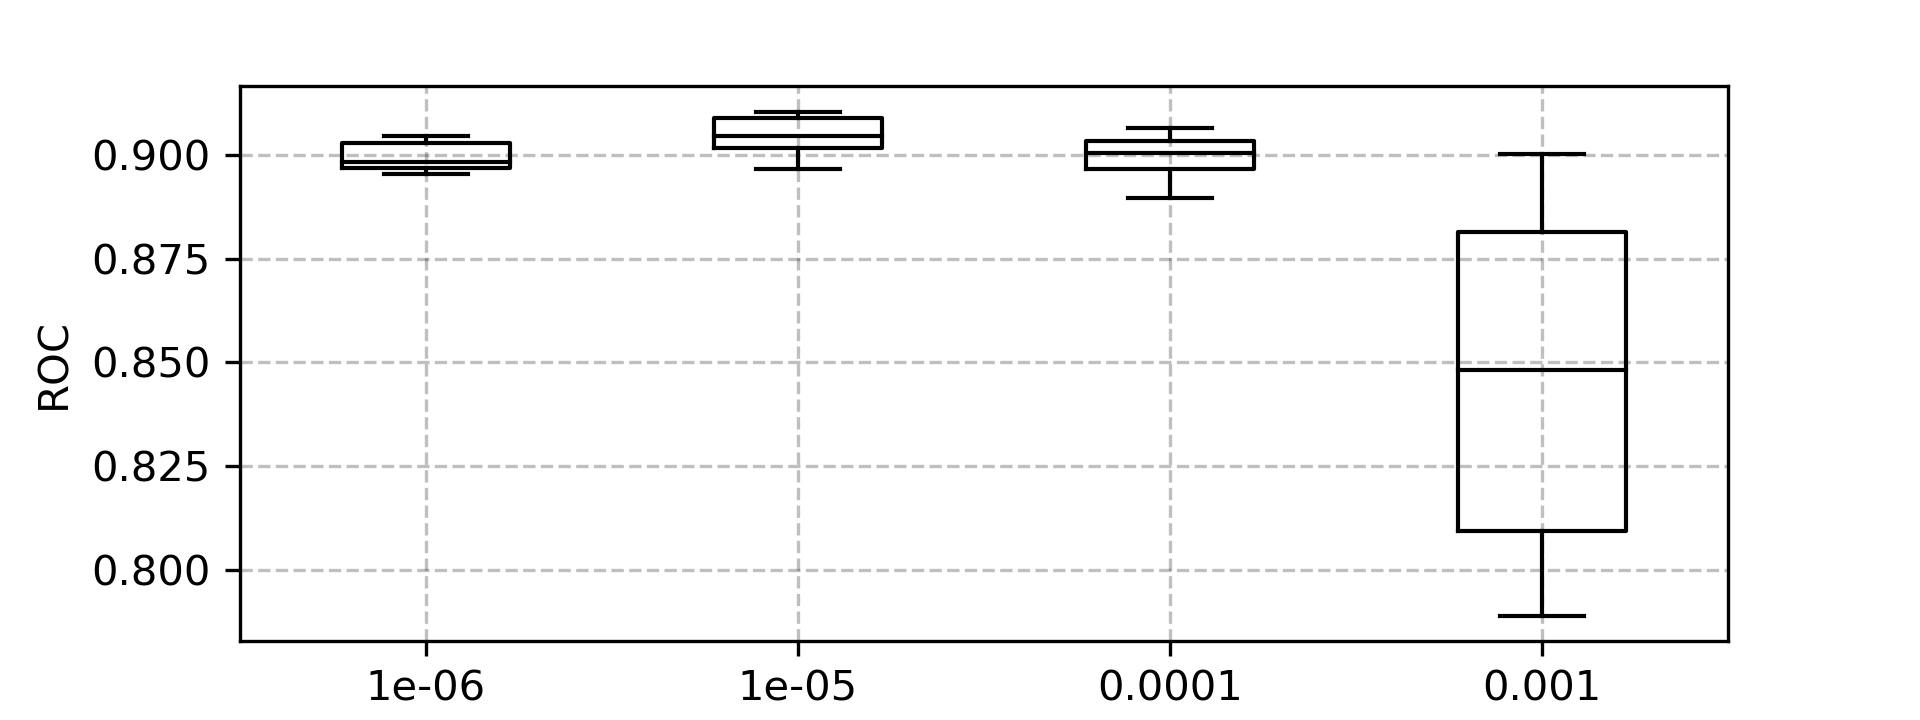
\includegraphics[scale=0.5]{images/all_plots/densenet121_patterns_no_aug_learning_rate.png}}
\subfigure[HumanLba]{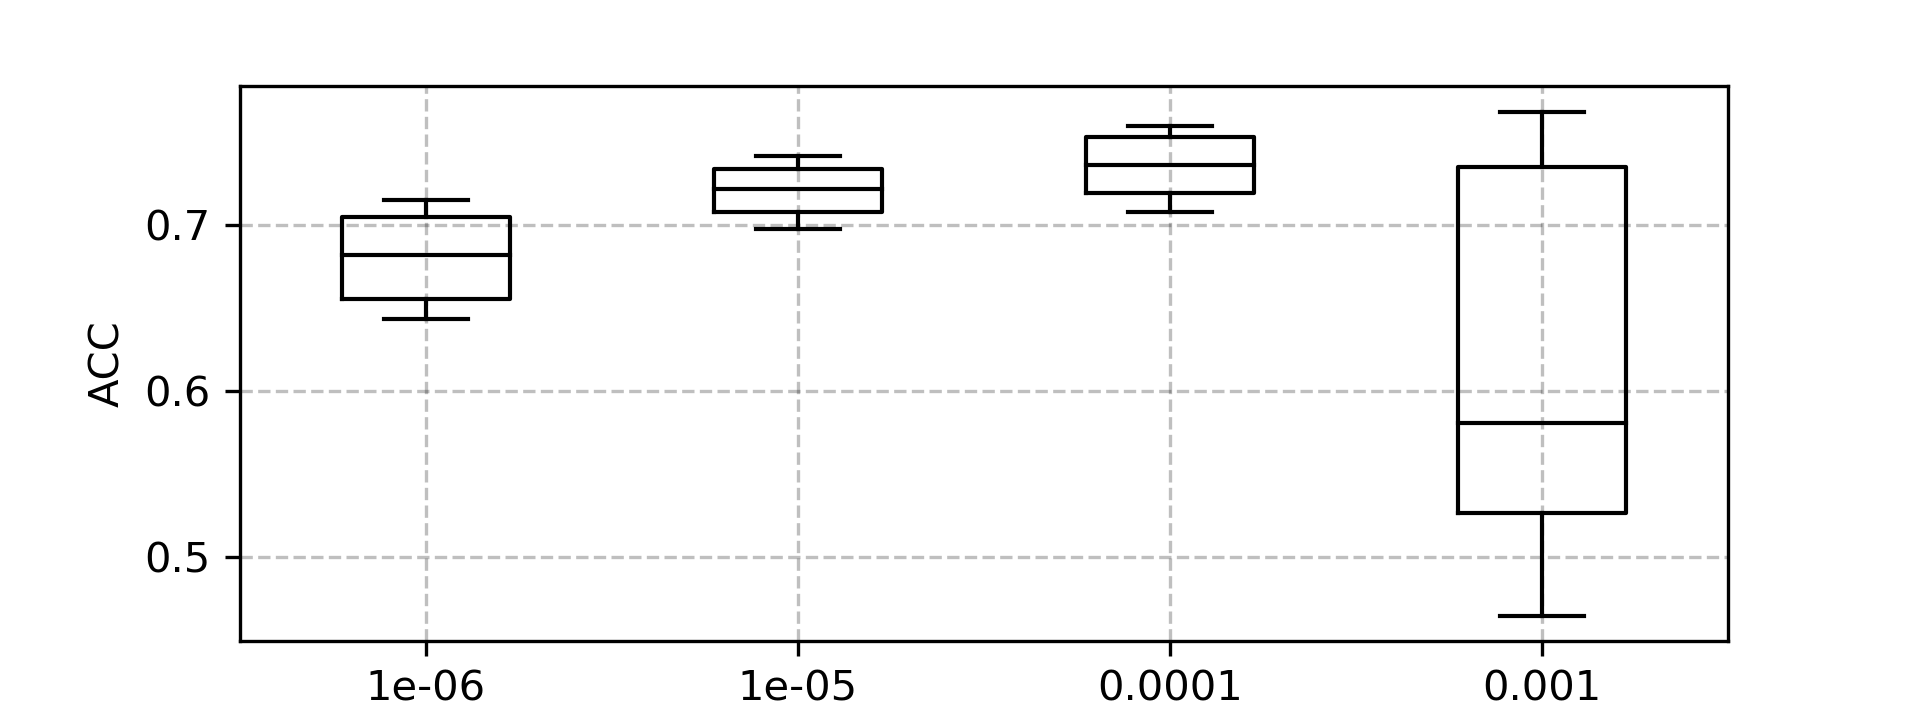
\includegraphics[scale=0.5]{images/all_plots/densenet121_ulb_anapath_lba_learning_rate.png}}\\
\subfigure[BoneMarrow]{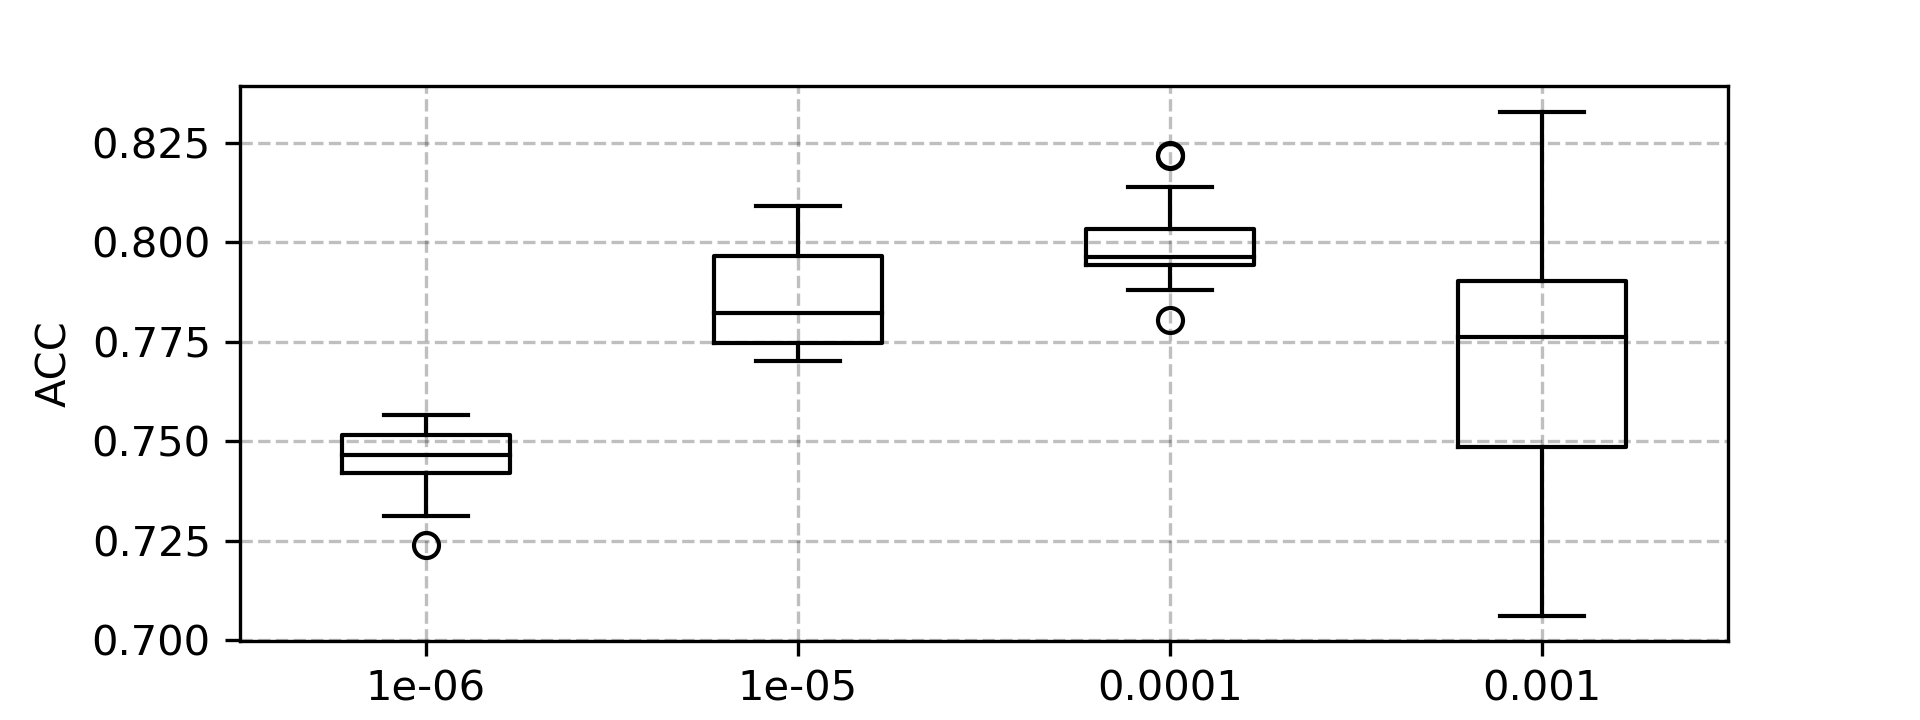
\includegraphics[scale=0.5]{images/all_plots/densenet121_ulg_bonemarrow_learning_rate.png}}
\subfigure[Breast1]{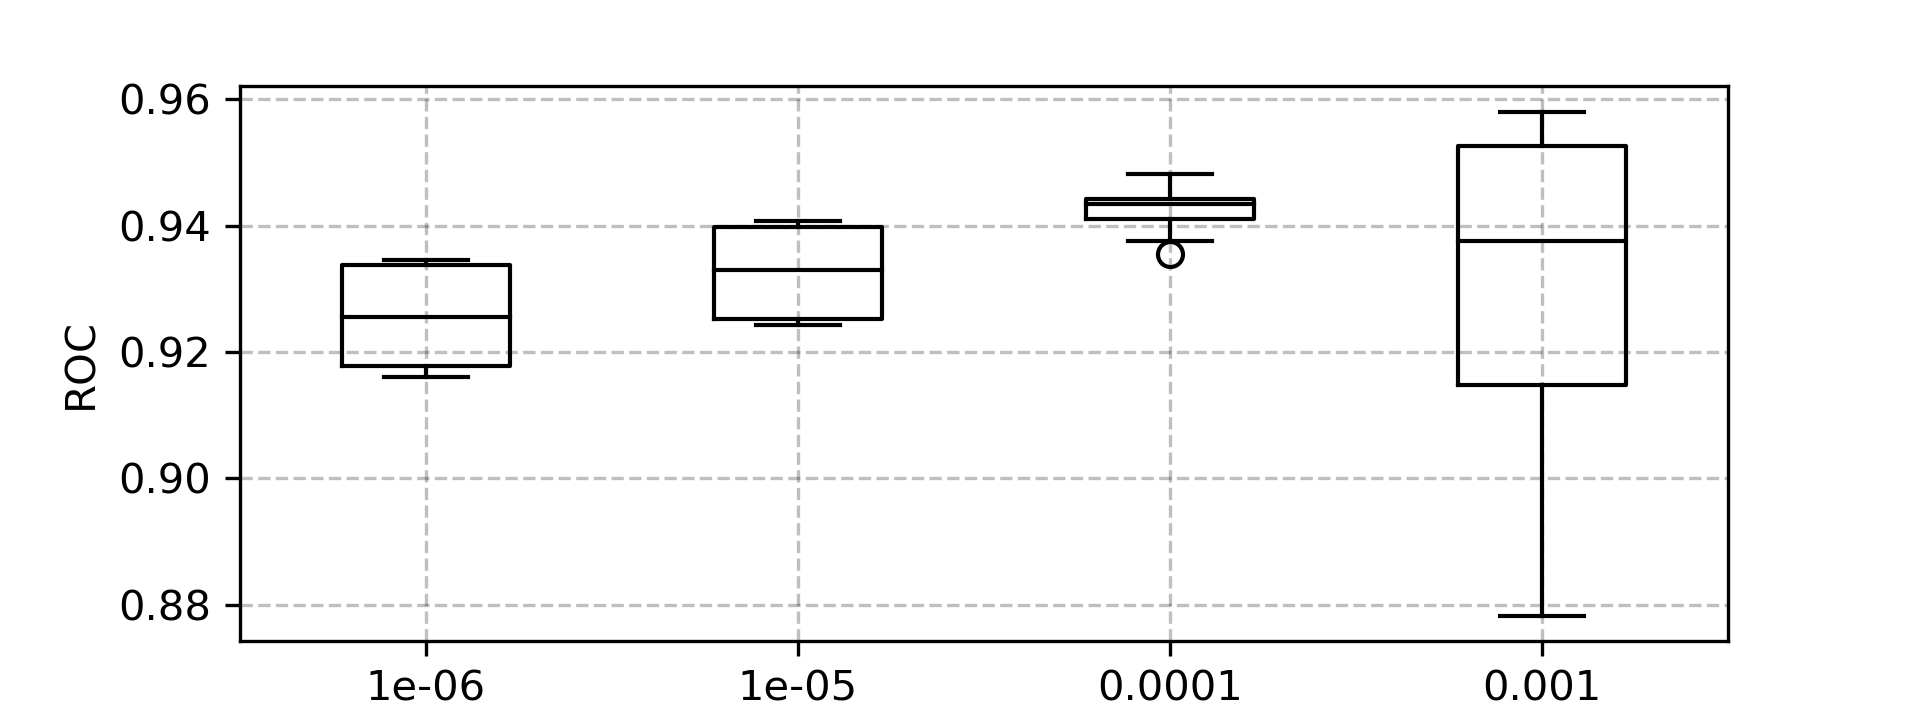
\includegraphics[scale=0.5]{images/all_plots/densenet121_ulg_breast_learning_rate.png}}\\
\subfigure[Breast2]{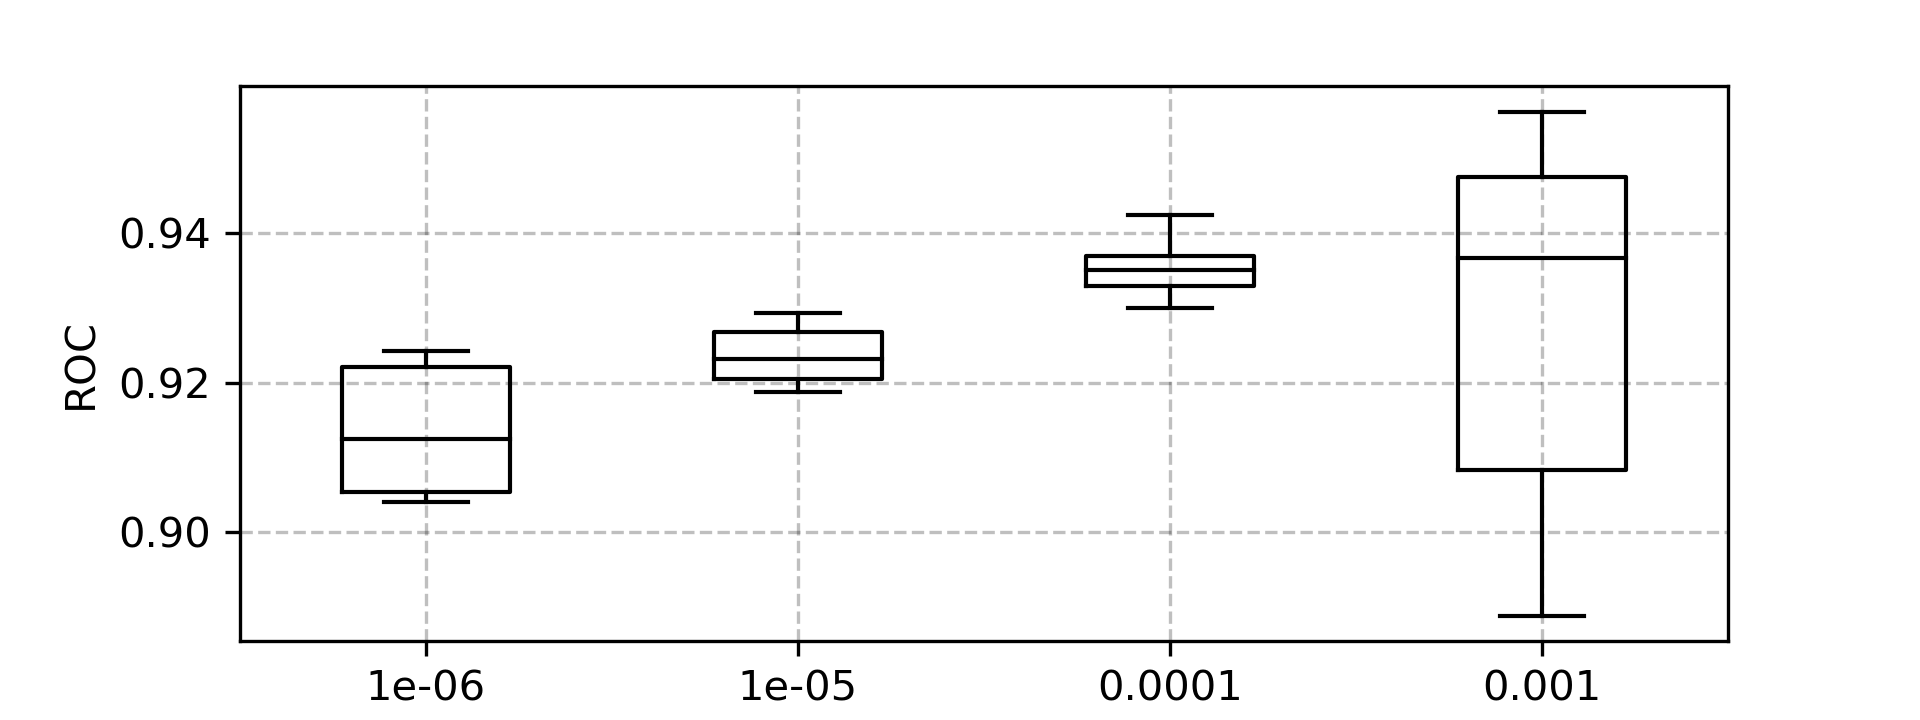
\includegraphics[scale=0.5]{images/all_plots/densenet121_ulg_breast2_learning_rate.png}}
\subfigure[Necrose]{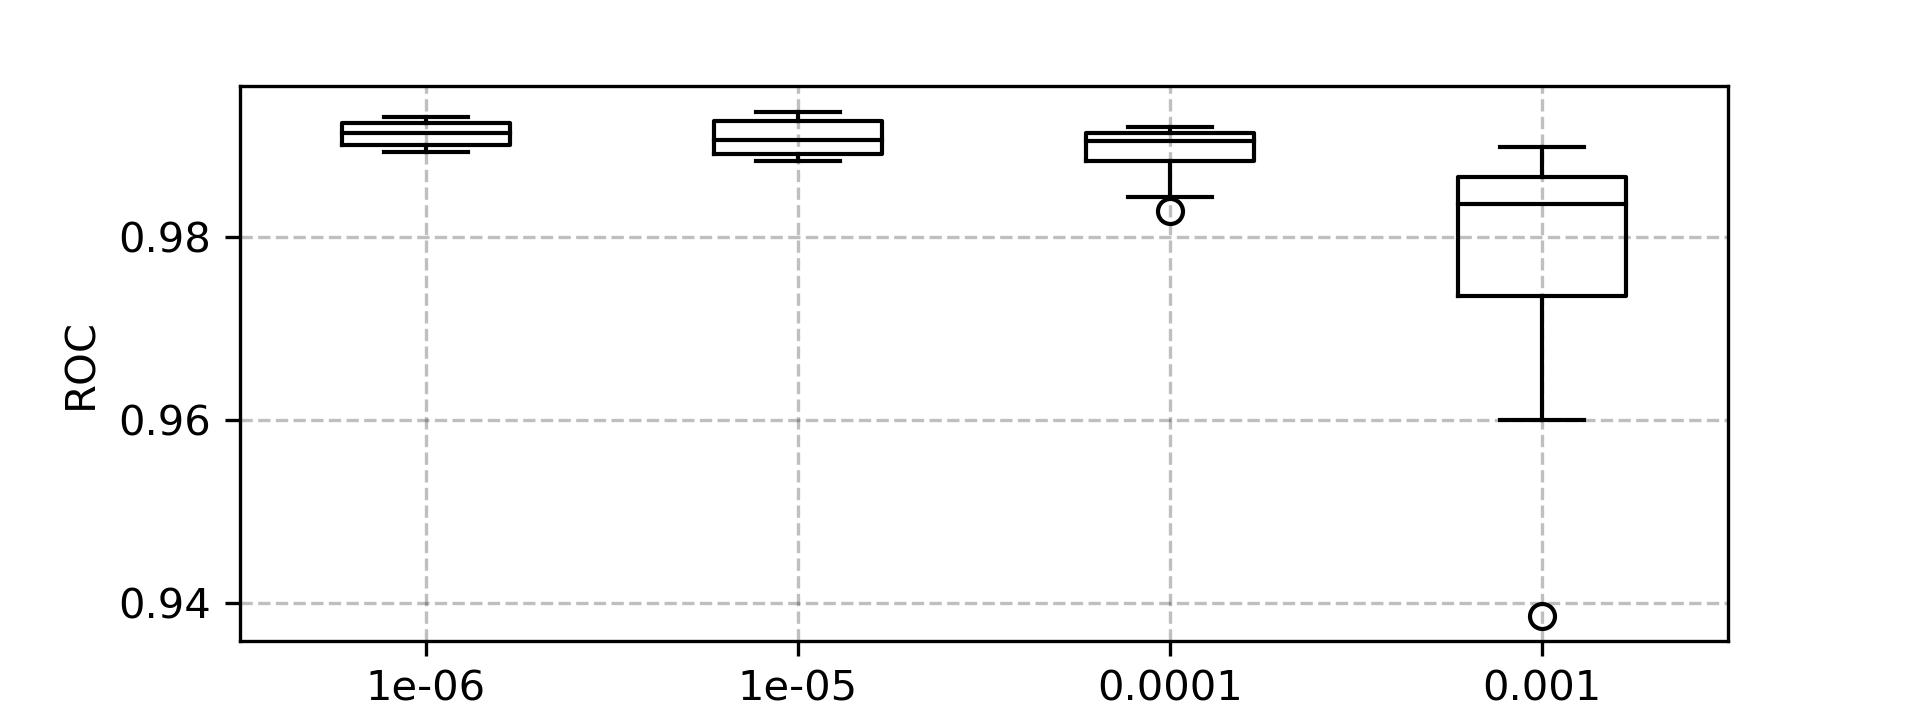
\includegraphics[scale=0.5]{images/all_plots/densenet121_ulg_lbtd2_chimio_necrose_learning_rate.png}}\\
\subfigure[MouseLba]{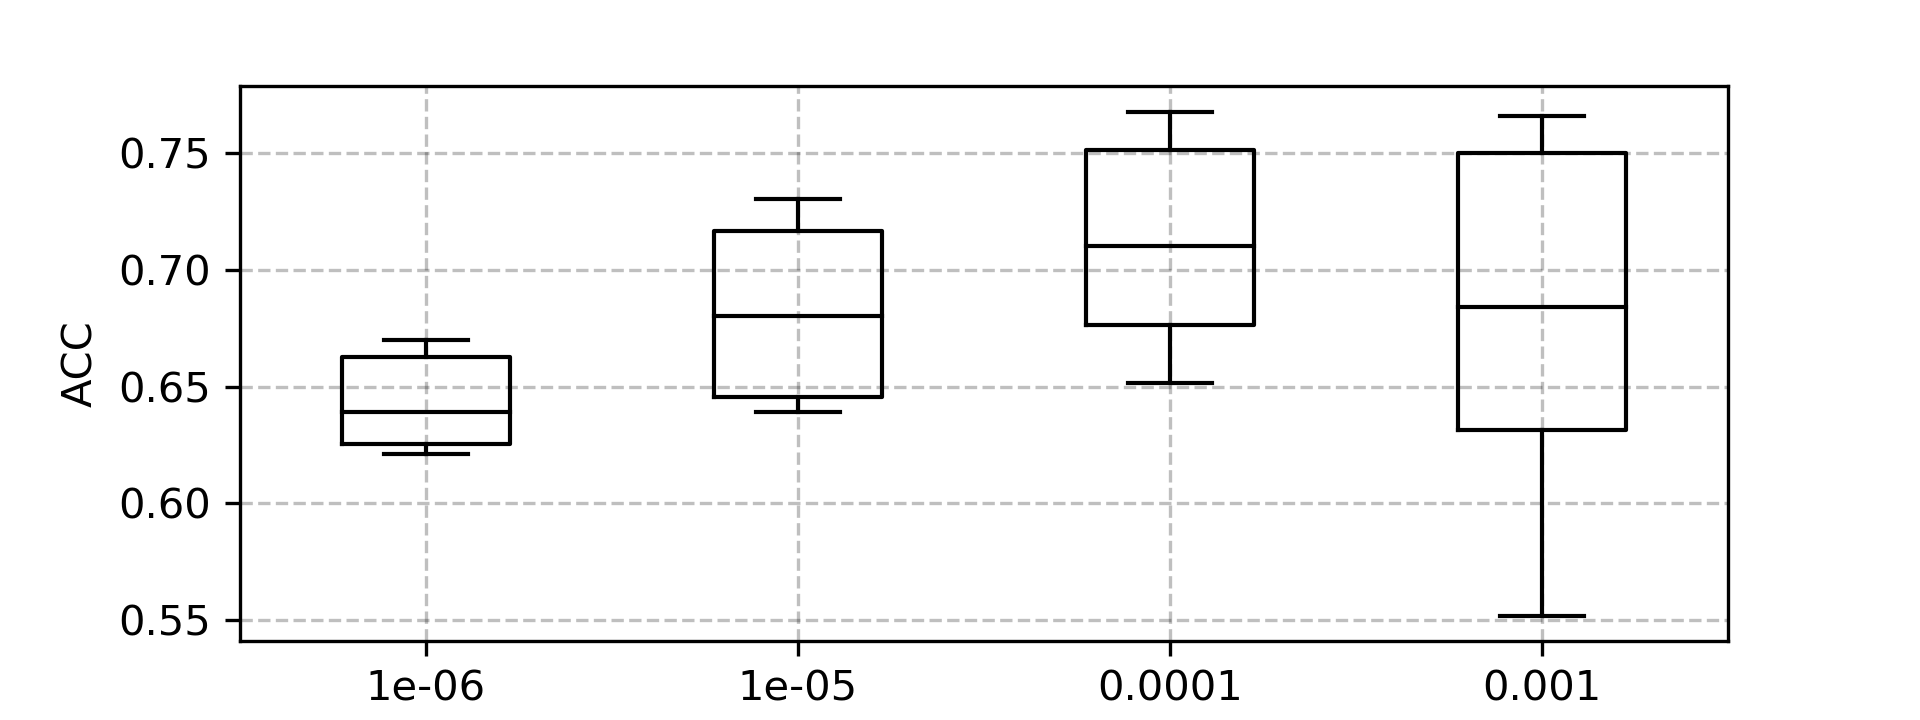
\includegraphics[scale=0.5]{images/all_plots/densenet121_ulg_lbtd_lba_learning_rate.png}}
\subfigure[Lung]{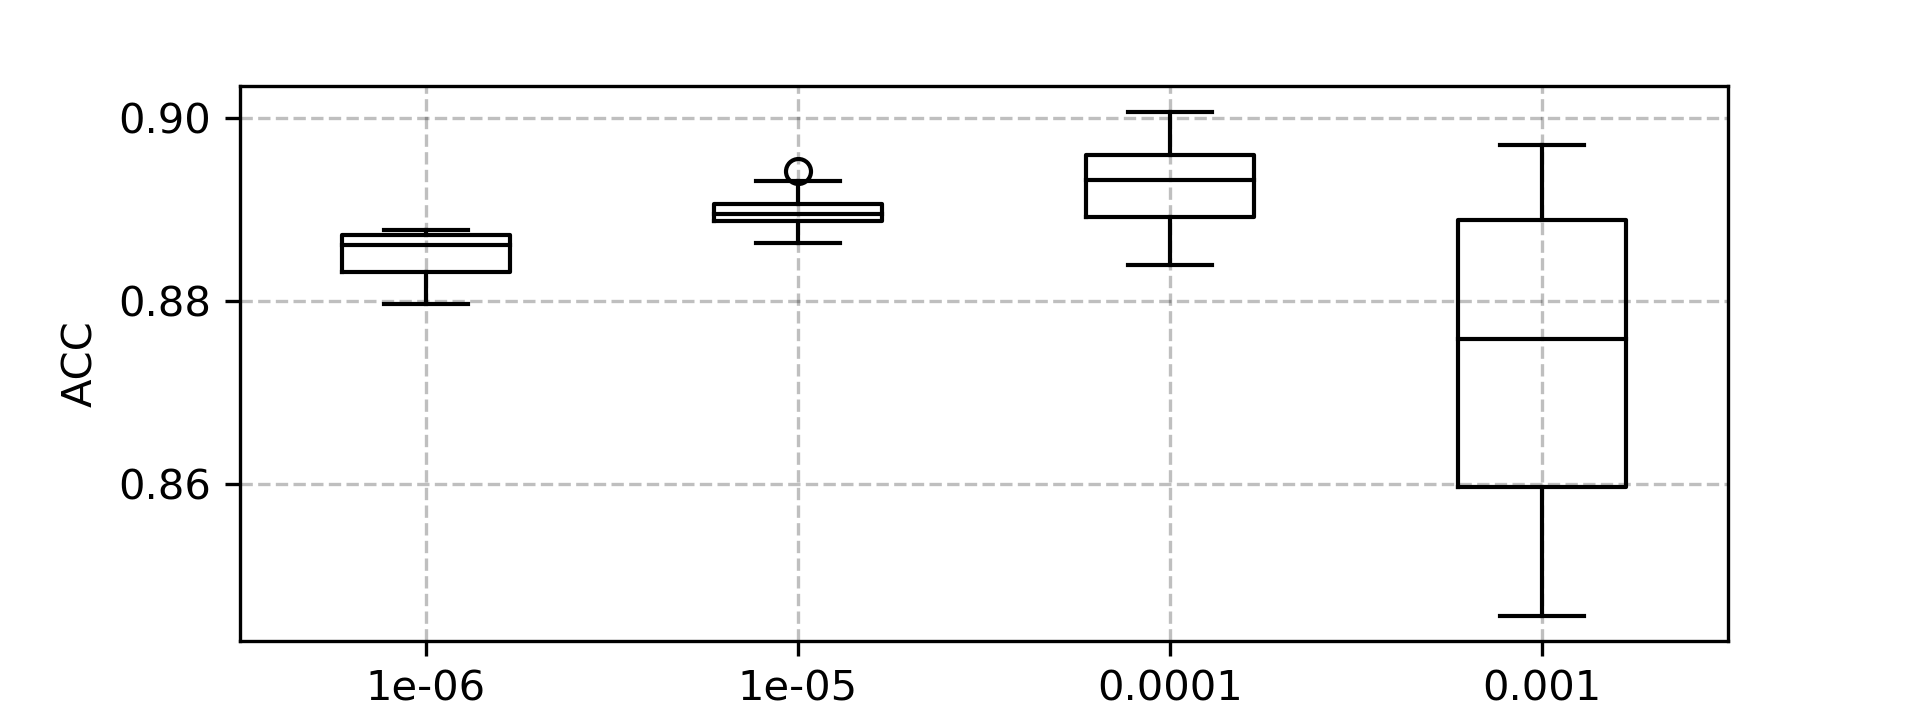
\includegraphics[scale=0.5]{images/all_plots/densenet121_ulg_lbtd_tissus_learning_rate.png}}
    \caption{Distributions of scores per learning rate on DenseNet121. Each boxplot results from the aggregation of the transfer scores of all models using the a learning rate value on the given network and dataset.}
    \label{app:mtask:fig:app:lr_densenet}
\end{figure*}

\begin{figure*}[h]
    \centering
\subfigure[CellInclusion]{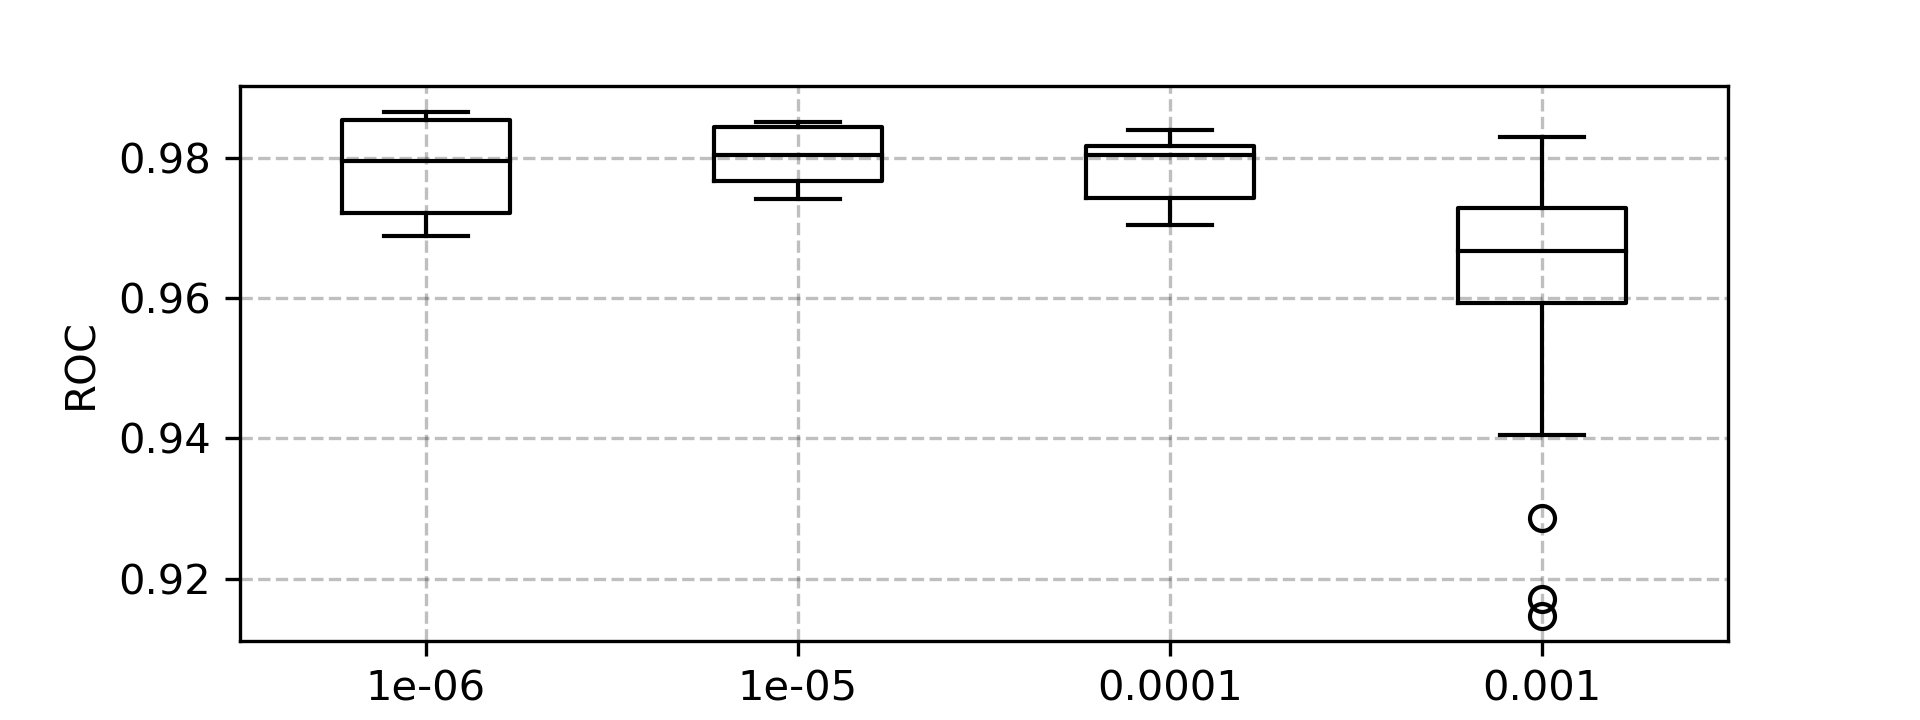
\includegraphics[scale=0.5]{images/all_plots/resnet50_cells_no_aug_learning_rate.png}}
\subfigure[Glomeruli]{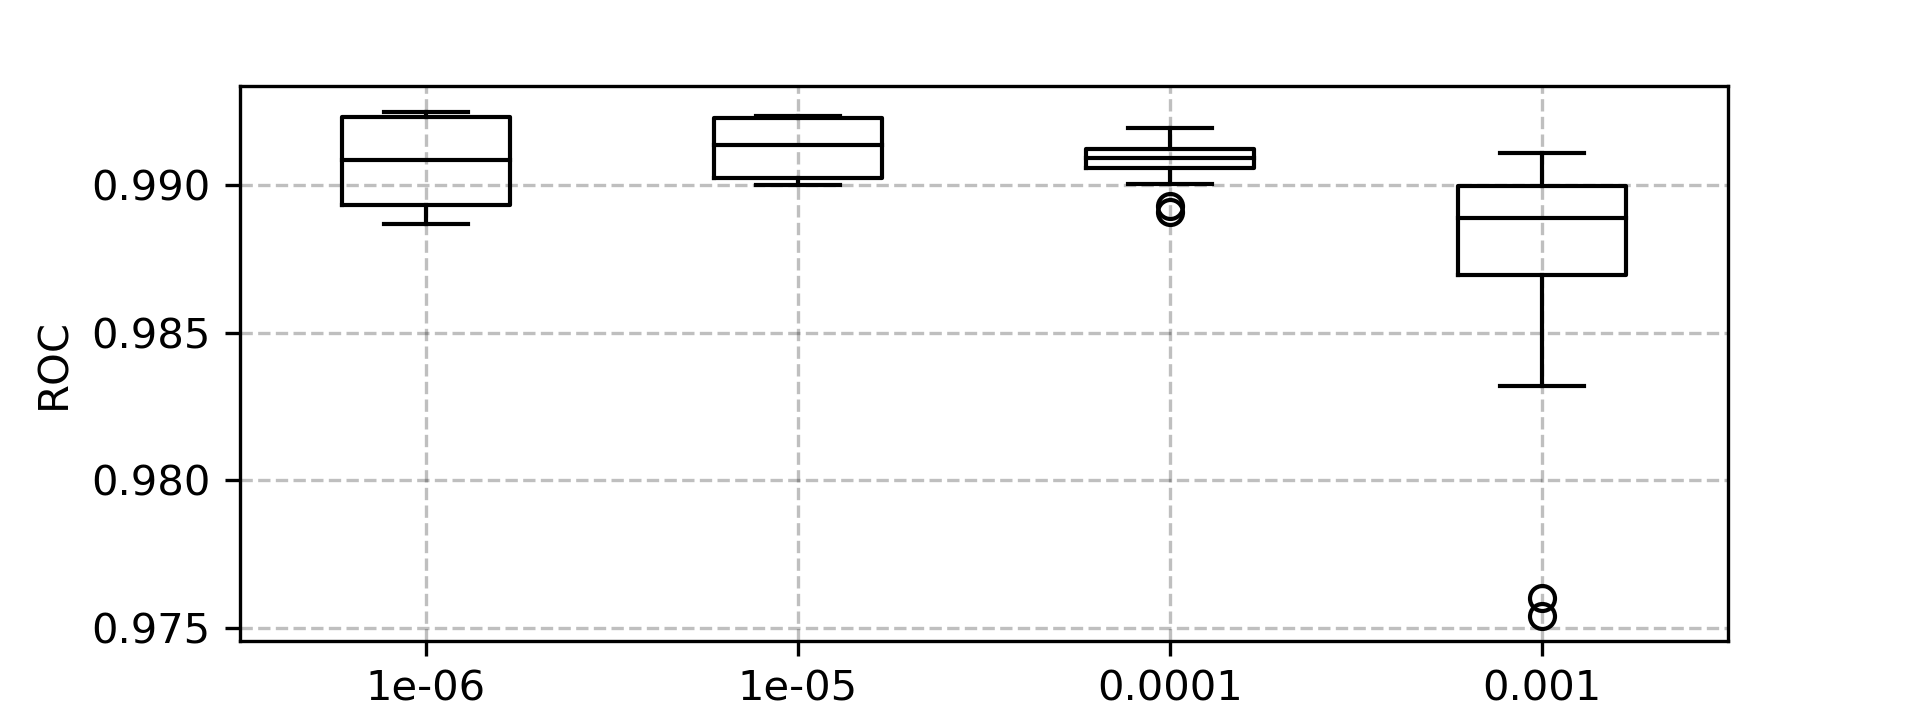
\includegraphics[scale=0.5]{images/all_plots/resnet50_glomeruli_no_aug_learning_rate.png}}\\
\subfigure[ProliferativePattern]{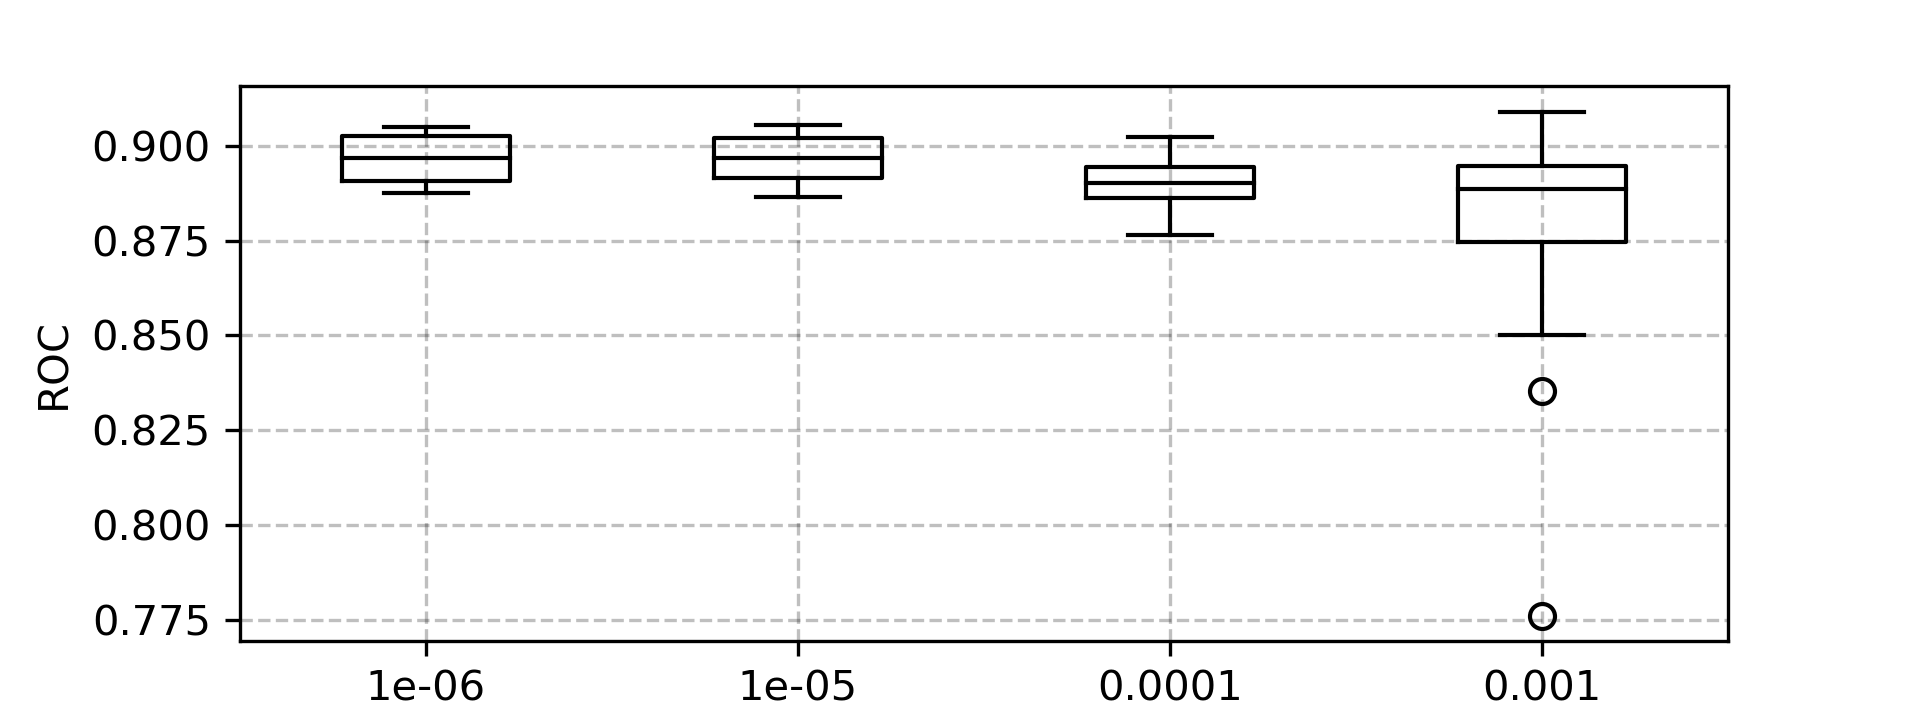
\includegraphics[scale=0.5]{images/all_plots/resnet50_patterns_no_aug_learning_rate.png}}
\subfigure[HumanLba]{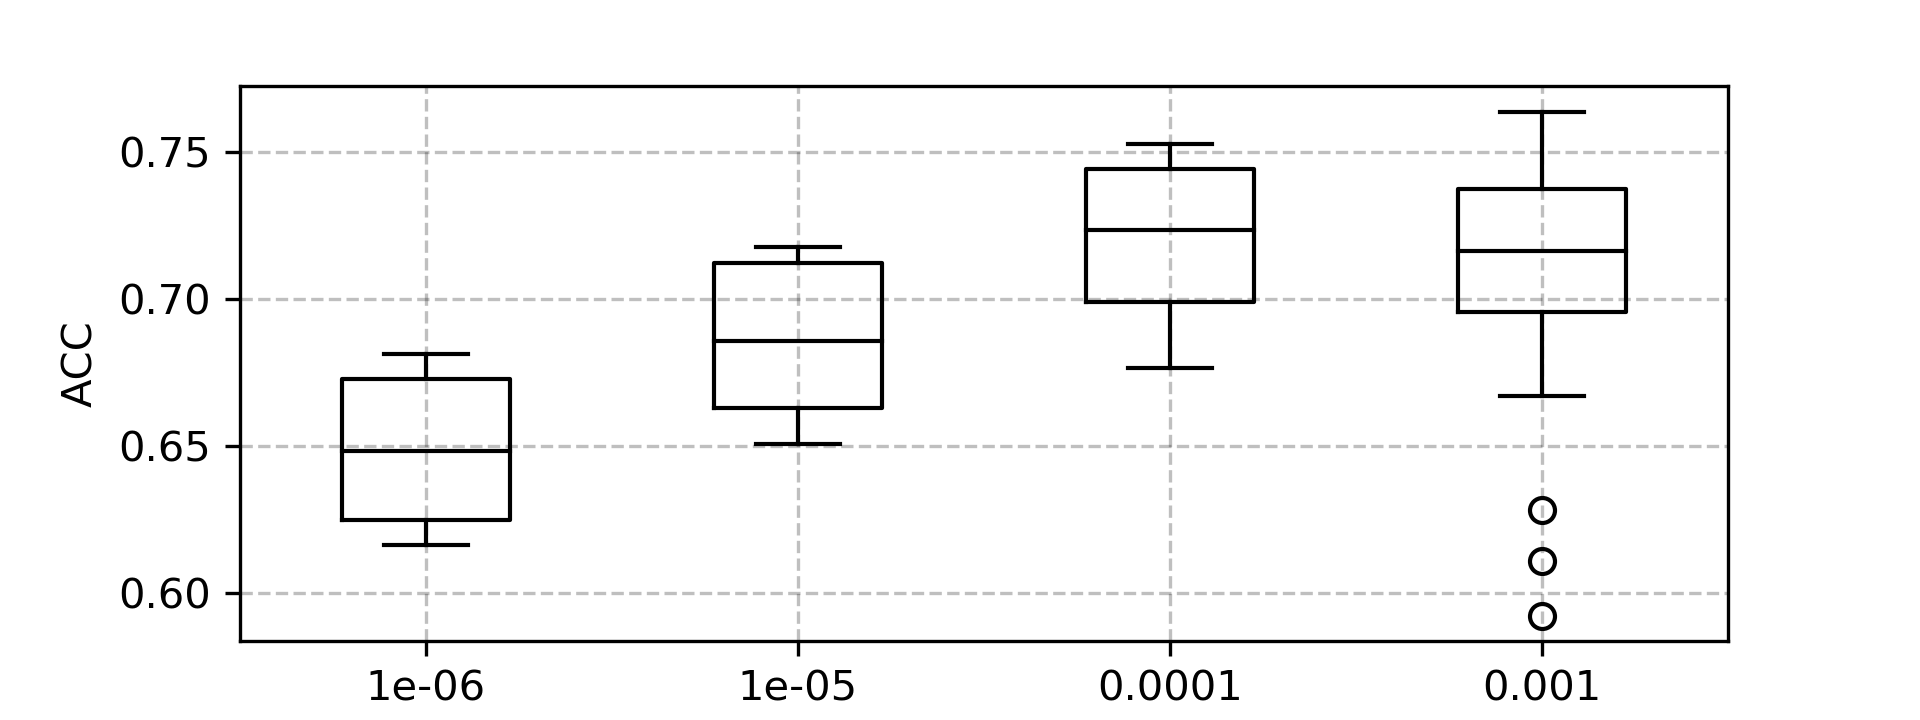
\includegraphics[scale=0.5]{images/all_plots/resnet50_ulb_anapath_lba_learning_rate.png}}\\
\subfigure[BoneMarrow]{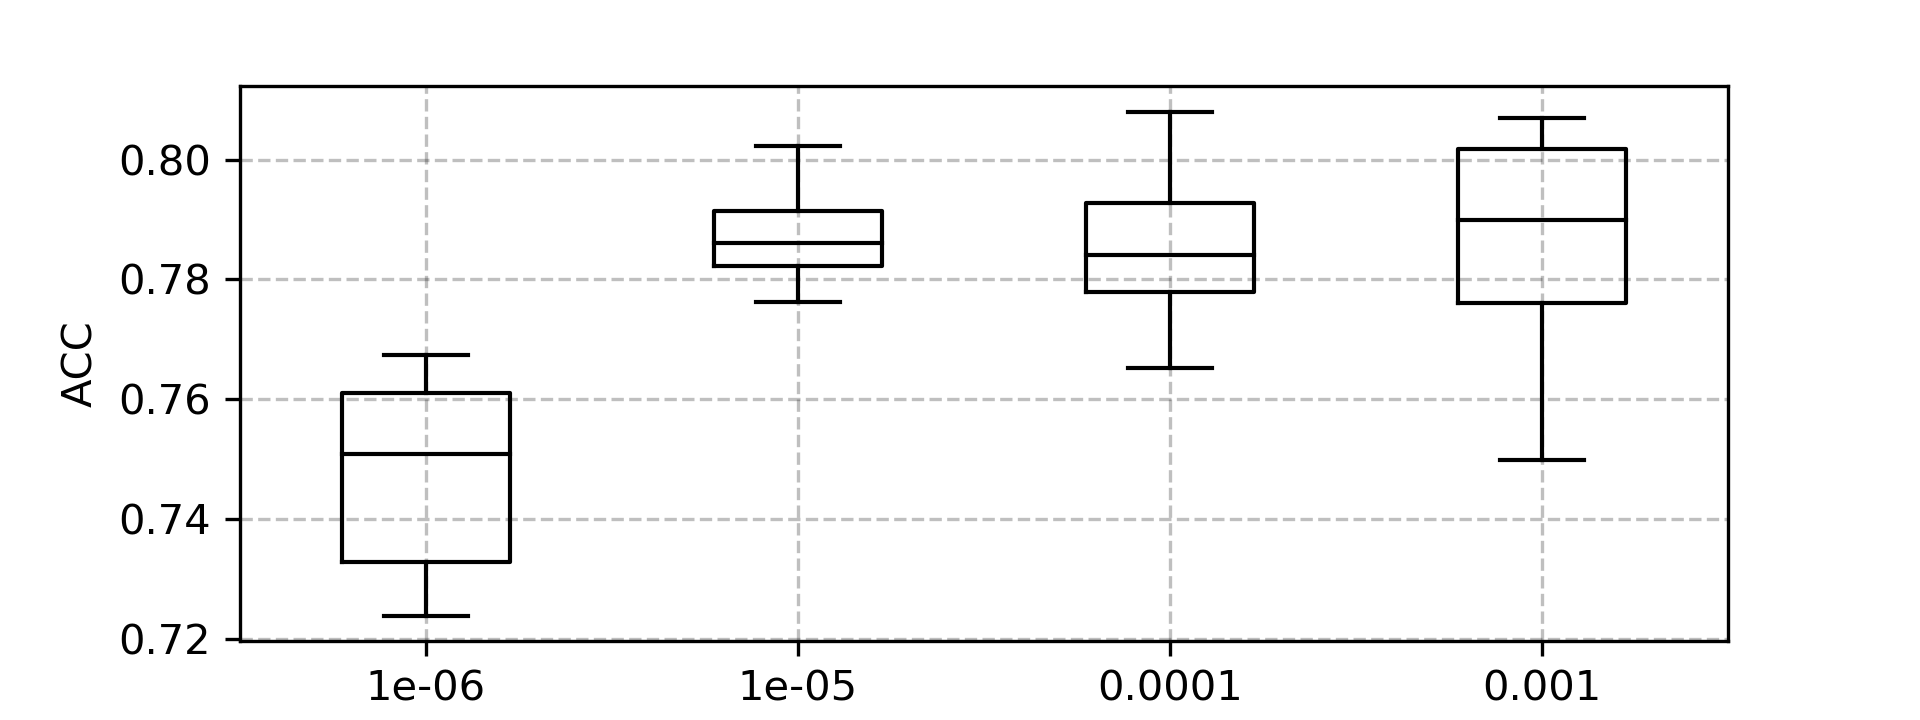
\includegraphics[scale=0.5]{images/all_plots/resnet50_ulg_bonemarrow_learning_rate.png}}
\subfigure[Breast1]{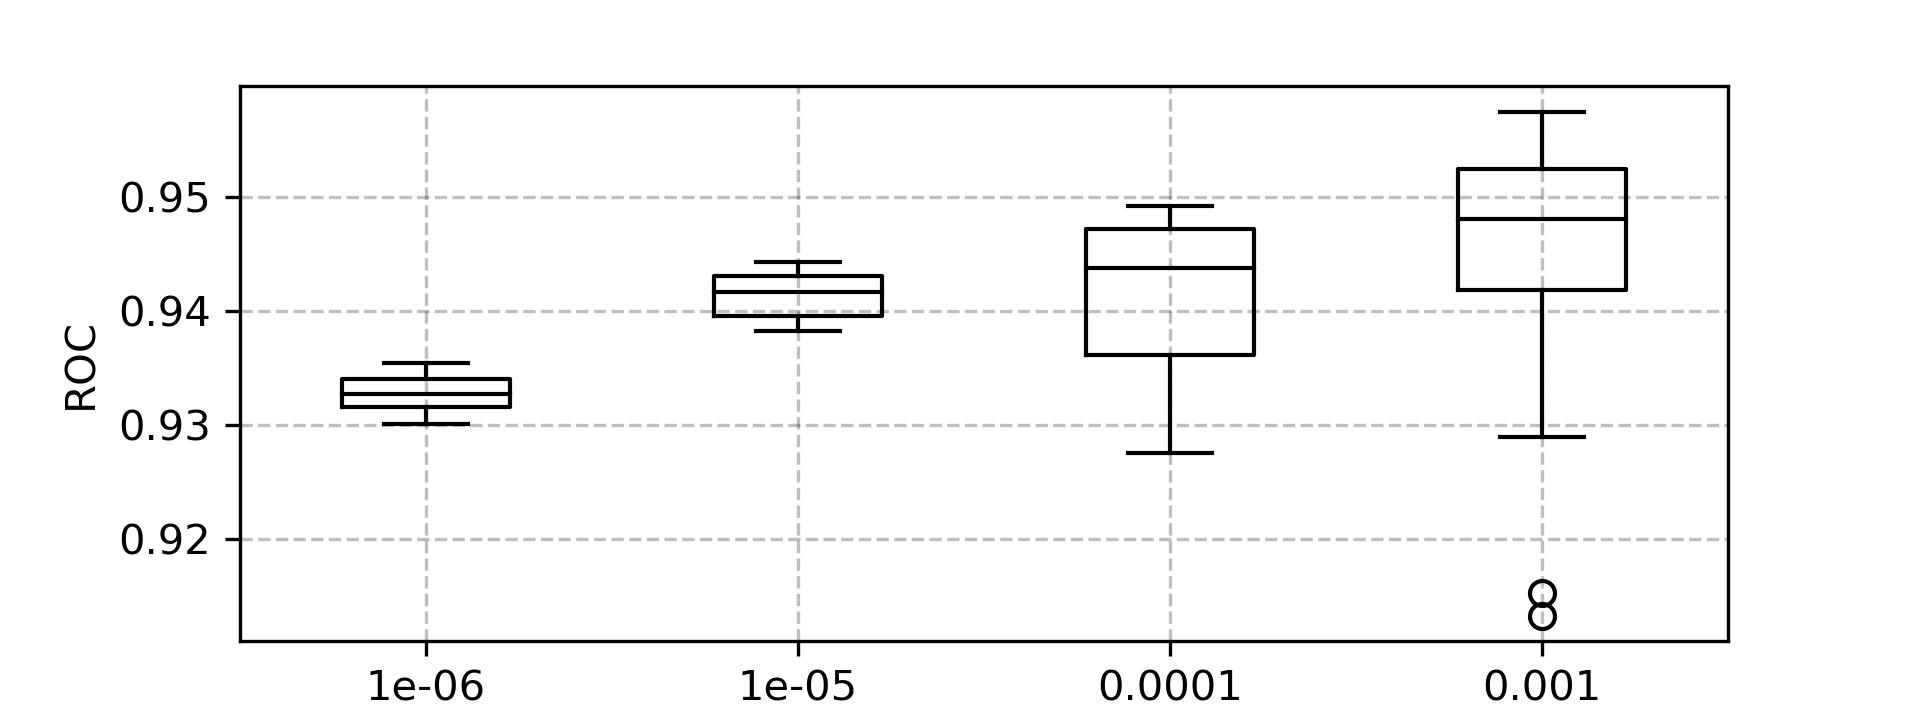
\includegraphics[scale=0.5]{images/all_plots/resnet50_ulg_breast_learning_rate.png}}\\
\subfigure[Breast2]{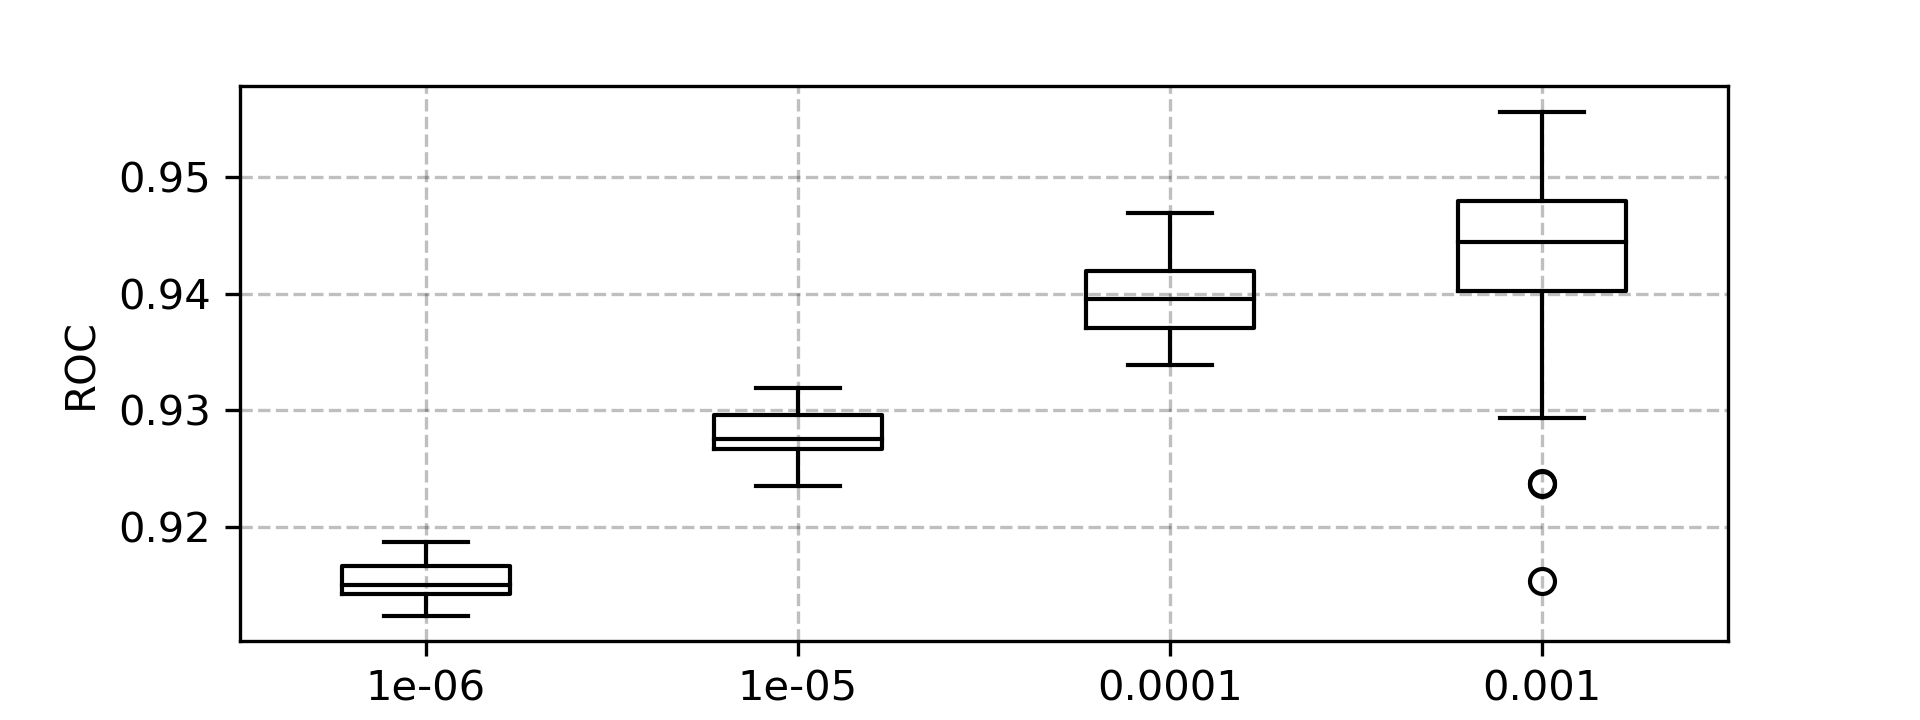
\includegraphics[scale=0.5]{images/all_plots/resnet50_ulg_breast2_learning_rate.png}}
\subfigure[Necrose]{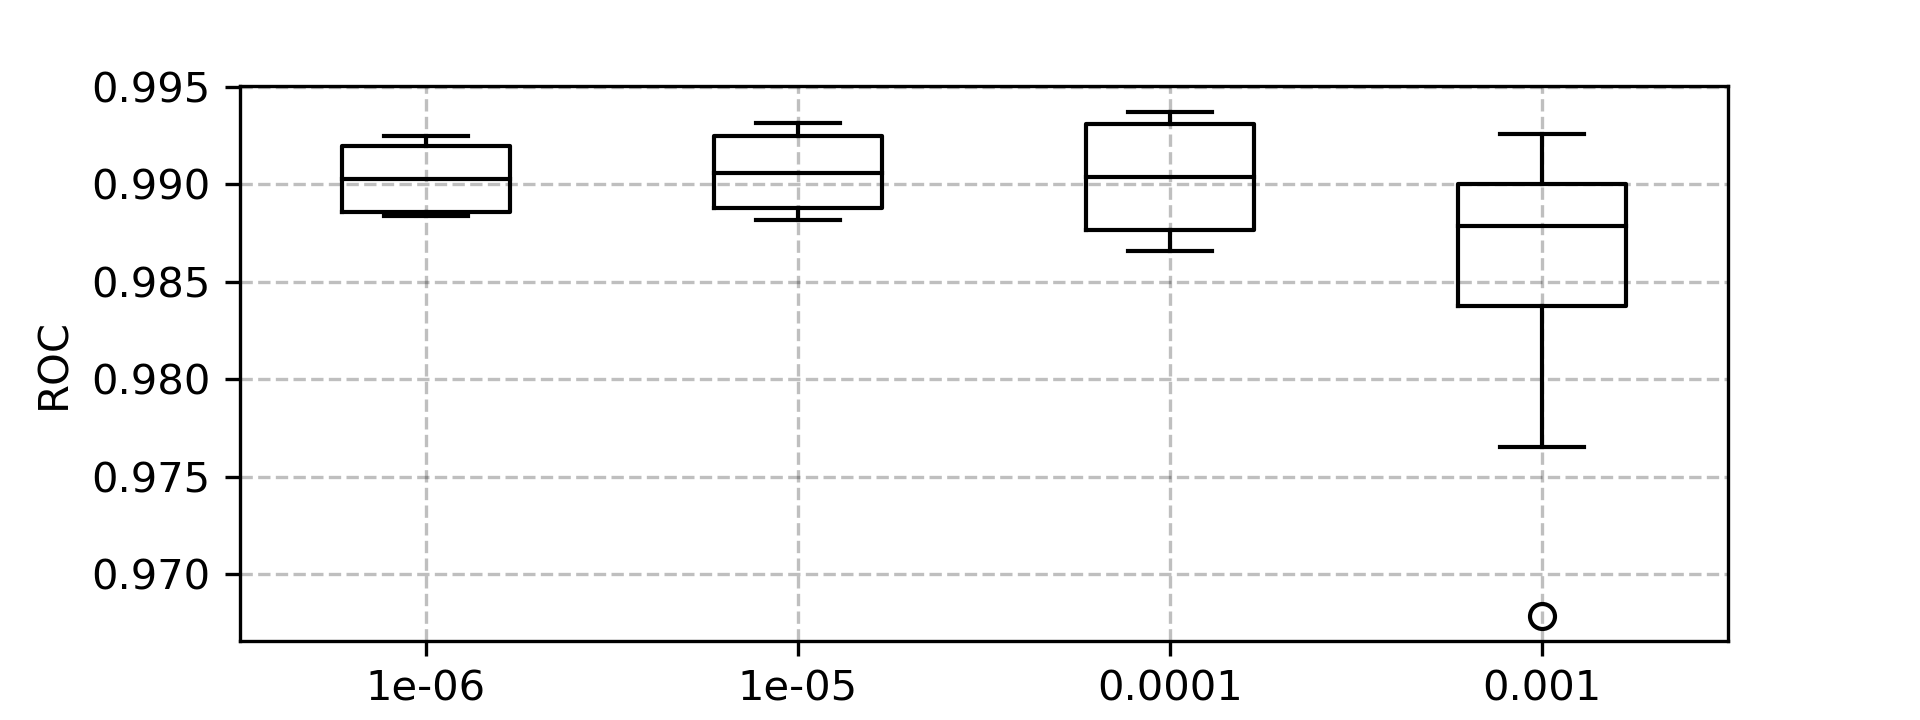
\includegraphics[scale=0.5]{images/all_plots/resnet50_ulg_lbtd2_chimio_necrose_learning_rate.png}}\\
\subfigure[MouseLba]{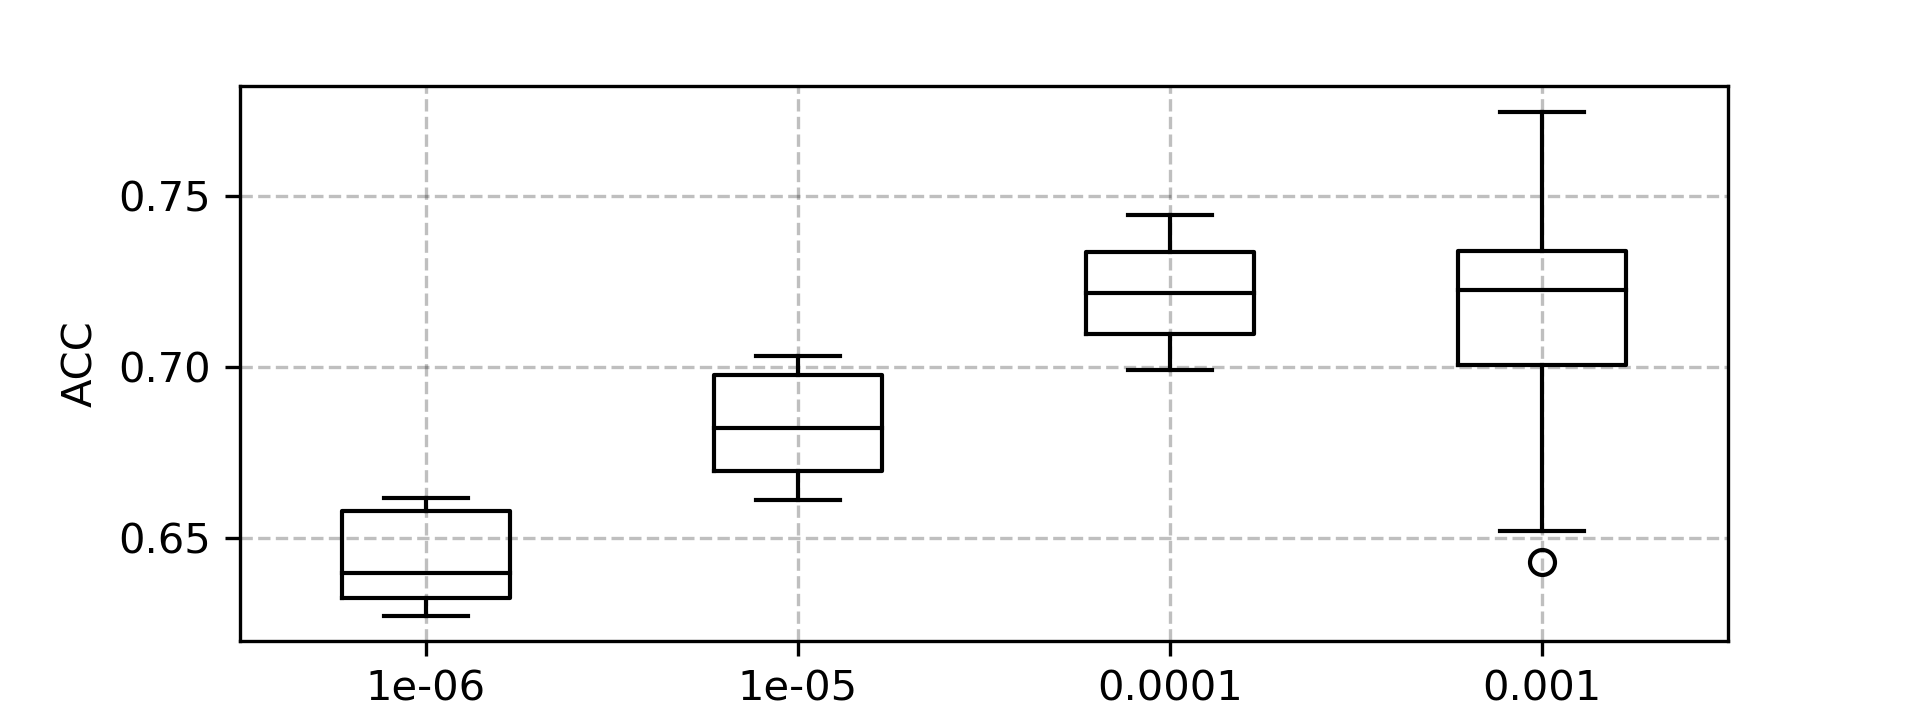
\includegraphics[scale=0.5]{images/all_plots/resnet50_ulg_lbtd_lba_learning_rate.png}}
\subfigure[Lung]{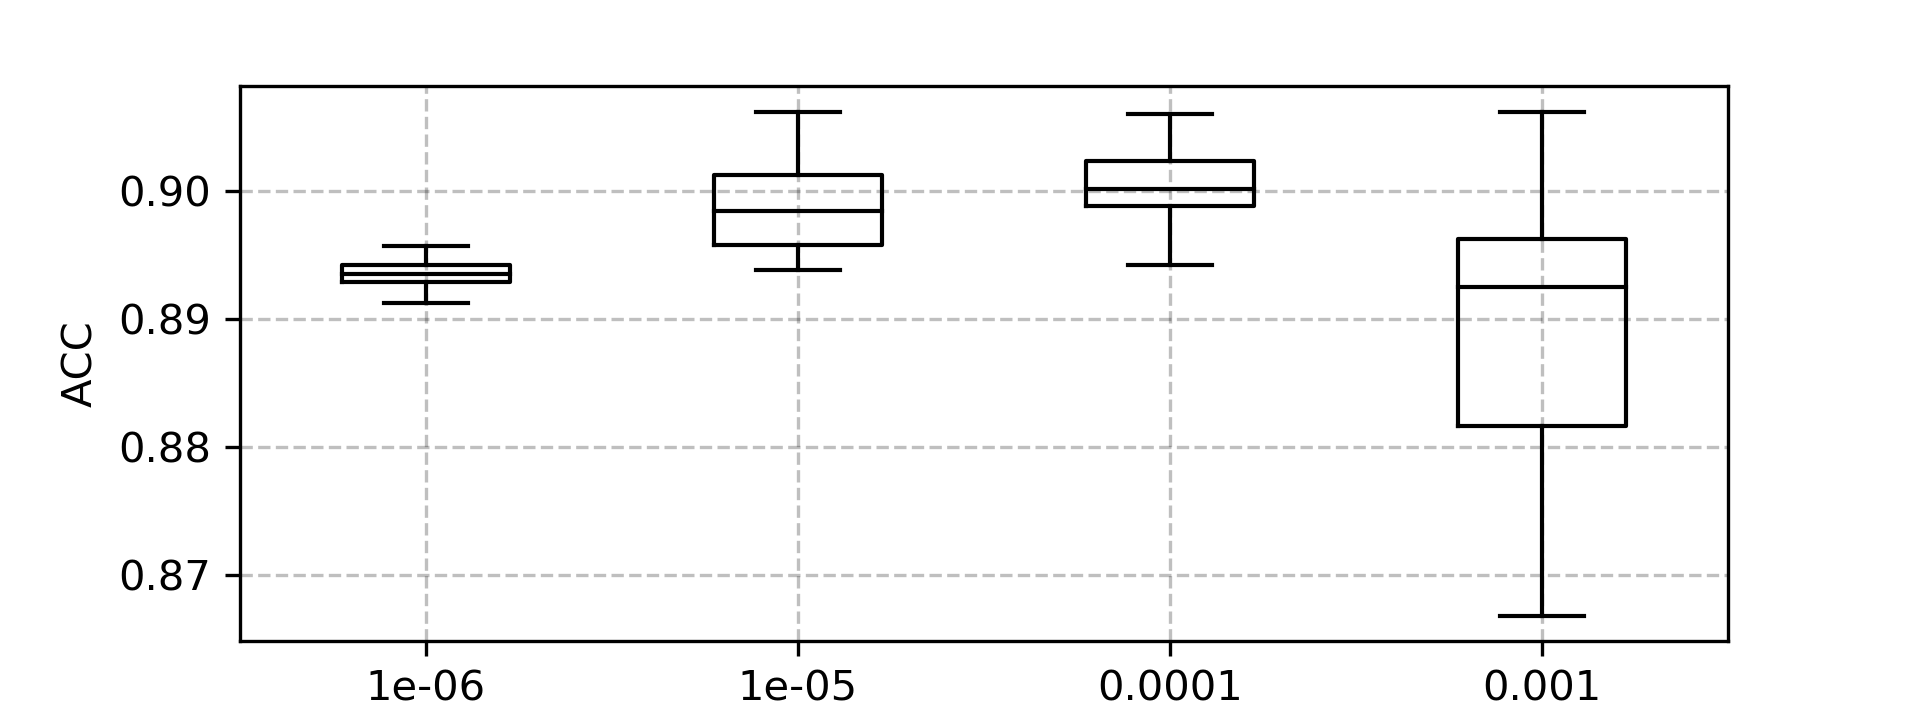
\includegraphics[scale=0.5]{images/all_plots/resnet50_ulg_lbtd_tissus_learning_rate.png}}
    \caption{Distributions of scores per learning rate on ResNet50. Each boxplot results from the aggregation of the transfer scores of all models using the a learning rate value on the given network and dataset.}
    \label{app:mtask:fig:app:lr_resnet}
\end{figure*}